\documentclass [MS] {UCLAthesis}

\graphicspath{ {figures/} }

\usepackage{xcolor}
\definecolor{codegreen}{rgb}{0,0.6,0}
\definecolor{codegray}{rgb}{0.5,0.5,0.5}
\definecolor{codepurple}{rgb}{0.58,0,0.82}
\definecolor{backcolour}{rgb}{0.95,0.95,0.92}

\usepackage{listings}
\lstdefinestyle{mystyle}{
    backgroundcolor=\color{backcolour},   
    commentstyle=\color{codegreen},
    keywordstyle=\color{magenta},
    numberstyle=\tiny\color{codegray},
    stringstyle=\color{codepurple},
    basicstyle=\ttfamily\footnotesize,
    breakatwhitespace=false,         
    breaklines=true,                 
    captionpos=b,                    
    keepspaces=true,                 
    numbers=left,                    
    numbersep=5pt,                  
    showspaces=false,                
    showstringspaces=false,
    showtabs=false,                  
    tabsize=2
}
\lstset{style=mystyle}

%%%%%%%%%%%%%%%%%%%%%%%%%%%%%%%%%%%%%%%%%%%%%%%%%%%%%%%%%%%%%%%%%%%%%%%%
%                                                                      %
%                          PRELIMINARY PAGES                           %
%                                                                      %
%%%%%%%%%%%%%%%%%%%%%%%%%%%%%%%%%%%%%%%%%%%%%%%%%%%%%%%%%%%%%%%%%%%%%%%%

\title          {Visual Tracking with Spiking Neural Networks in a Biomimetic Model of the Eye}
\department     {Computer Science}
\author         {Taasin Saquib}
\degreeyear     {2022}

%%%%%%%%%%%%%%%%%%%%%%%%%%%%%%%%%%%%%%%%%%%%%%%%%%%%%%%%%%%%%%%%%%%%%%%%

\chair          {Demetri Terzopoulos}
\member         {Jonathan Kao}
\member         {Sriram Sankararaman}

%%%%%%%%%%%%%%%%%%%%%%%%%%%%%%%%%%%%%%%%%%%%%%%%%%%%%%%%%%%%%%%%%%%%%%%%

\dedication     {\textsl{dedication}}

%%%%%%%%%%%%%%%%%%%%%%%%%%%%%%%%%%%%%%%%%%%%%%%%%%%%%%%%%%%%%%%%%%%%%%%%

\acknowledgments {I would like to dedicate this section to all that made the work of this thesis possible. First, I am grateful for Professor Demetri Terzopoulos' support and guidance in designing this project. I thank all of my colleagues at UCLA Computer Graphics \& Vision Laboratory for their help and interactions. I also acknowledge that the work of this thesis is built upon the work of Arjun Lakshmipathi who created the biomimetic eye model and Dr. Masaki Nakada and/or Honglin Chen who created the LiNet and data collection methods for the eye. Thanks to both Arjun and Dr. Nakada for their guidance and willingness to help.}

%%%%%%%%%%%%%%%%%%%%%%%%%%%%%%%%%%%%%%%%%%%%%%%%%%%%%%%%%%%%%%%%%%%%%%%%

\vitaitem   {2017}
                {Full Stack Software Engineering Intern, Project Looma, 
                Village Tech Solutions, Palo Alto, California.}
\vitaitem   {2018}
                {Software Engineering Intern, Device Drivers, 
                Nvidia, Santa Clara, California.}
\vitaitem   {2019}
                {Software Engineering Intern, Device Drivers, 
                Nvidia, Santa Clara, California.}
\vitaitem   {2020}
                {B.S.~(Computer Science and Engineering),
                University of California, Los Angeles.}
\vitaitem   {2020}
                {Software Engineering Intern, Traffic Engineering, 
                Splunk, San Jose, California.}
\vitaitem   {2020--present}
                {Teaching Assistant, Computer Science Department, UCLA. 
                Taught CS 31 (Introduction to Computer Science I) under direction of Professor David Smallberg (Fall '20). 
                Taught CS 32 (Introduction to Computer Science II) under direction of Professor David Smallberg (Winter '21, Spring '21). 
                Taught CS M51A (Logic Design of Digital Systems) under direction of Professor Richard Korf (Fall '21).}
\vitaitem   {2020--present}
                {Graduate Researcher, Computer Graphics and Vision Lab, 
                Computer Science Department, University of California, Los Angeles.}

%%%%%%%%%%%%%%%%%%%%%%%%%%%%%%%%%%%%%%%%%%%%%%%%%%%%%%%%%%%%%%%%%%%%%%%%

\abstract {
Spiking neural networks (SNNs) are hailed as the next wave of deep learning. Inspired by the brain, they promise low latency and low power usage when run on neuromorphic hardware. Current computer vision models have made great progress but often require power hungry GPUs to train and run, making them great candidates to replace with SNNs. This thesis specifically trains an SNN to work with a biomimetic eye model that can track a target through space. While many SNNs are converted from trained artificial neural networks (ANNs), we train our models from scratch using modified deep learning techniques. In addition, object tracking is a regression task; classification tasks are easier to implement with SNNs and have received more attention from researchers. We use surrogate gradients and insert a linear layer to convert membrane voltages from the last spiking layer into our desired outputs. Also, inspired by the ON and OFF bipolar cells of the retina, we use event-based data to control the eye. Our SNN is slightly noisier than the previously used LiNet architecture but still successfully tracks the ball through various trajectories and maintains the eye's bioimimetic properties.
}

%%%%%%%%%%%%%%%%%%%%%%%%%%%%%%%%%%%%%%%%%%%%%%%%%%%%%%%%%%%%%%%%%%%%%%%%

\begin {document}
\makeintropages

%%%%%%%%%%%%%%%%%%%%%%%%%%%%%%%%%%%%%%%%%%%%%%%%%%%%%%%%%%%%%%%%%%%%%%

\chapter{Introduction}

The human visual system is an astounding computational machine. Photons of light hit the retina and are processed to allow humans to do multiple tasks with high precision. Additionally, the visual cortex (V1) completes these tasks quickly and with little energy. Computer vision algorithms have come very far in re-creating the performance of V1 in terms of accuracy, but require the use of power-hungry GPUs that lag behind the power and latency performance of the brain.

Spiking neural networks (SNNs), hailed as the “third wave of deep learning,” offer a more biologically inspired neuron model that consumes much less power than the standard artificial neurons currently in use. Many traditional AI tasks can be completed with SNNs using the right hardware in the form of neuromorphic chips and new training techniques. This thesis explores training a SNN to track a virtual target using a biomimetic eye model.

%********************************************************************%

\section{Contributions of the Thesis}

To be more precise, the contributions of this thesis are as follows:

\begin{itemize}
    \item We find a SNN architecture than can solve a regression task, which is more difficult than the more popular classification tasks.
  \item We train a SNN from scratch.
  \begin{itemize}
    \item We choose between rate and latency encoding, the two most commonly used encoding methods. We find the best encoding parameters for each encoding method.
    \item We use a surrogate gradient to solve the dead neuron problem and allow for the use of standard deep learning optimization techniques.
  \end{itemize}
  \item We turn the eye into an event-based model that only looks at what has changed in the scene. This is more biologically accurate and creates more sparse input to the model.
\end{itemize}

The original thesis of \citet{Arjun} tests the eye on different types of eye movements to demonstrate its biological accuracy. We also use these movements (saccade, fixation, and smooth pursuit) to test our SNN's performance on both normal and event-based data.

%********************************************************************%

\section{Overview}

The remaining sections of this thesis are organized as follows:

Chapter 2: A survey of relevant literature related to the use of SNNs in computer vision.

Chapter 3: We lay out the visual tracking task that we are trying to solve and detail the biomimetic eye model that we work with.

Chapter 4: We compare artificial neurons to spiking neurons and detail how SNNs operate.

Chapter 5: We detail how to encode light seen at the retina into spiking inputs for our SNN.

Chapter 6: We describe the architecture of our SNN along with training techniques.

Chapter 7: We report our results and compare our SNN performance to that of the existing LiNet architecture.

Chapter 8: We present our conclusions and offer ideas for future work.

%%%%%%%%%%%%%%%%%%%%%%%%%%%%%%%%%%%%%%%%%%%%%%%%%%%%%%%%%%%%%%%%%%%%%%

\chapter{Related Work}

Our work in this thesis is inspired by the prior work of \citet{Arjun_thesis}, who created the comprehensive eye model with realistic organs. This system was controlled by either inverse dynamics or a series of neural networks. The neural network of interest in this thesis, the LiNet foveation controller, was developed by Honglin Chen \citep{Arjun}. Both of these contributions improve upon the simple eye model created as part of the biomimetic human in \citet{Masaki}.

While the model of \citet{Arjun} can re-create realistic eye motion, the artificial neurons used as part of the neural networks are still high-level abstractions of actual neurons. This thesis pushes the eye to be more biologically realistic with the use of spiking neurons in spiking neural networks (SNNs). We explore how to encode our data into spikes, which is the job of photoreceptors in the mammalian retina; it is still unclear whether the visual system uses rate or latency encoding \citep{encoding_retina}, both of which are considered in this work. In addition, we train our SNNs on event-based data which emulates the ON-OFF bipolar cells of the retina. Packaging these two features along with a biologically inspired SNN will significantly add to the biological realism of the previous eye model \citep{Arjun}.

The remainder of this section overviews research related to SNNs.

%********************************************************************%

\section{Neuromorphic Hardware}

Hardware tailored to run SNNs is referred to as ``neuromorphic''. These chips take advantage of the fact that spiking activation functions only output 1's and 0's to operate with lower power consumption. They are also optimized for the asynchronous nature of spikes and can run new types of learning algorithms. Currently, GPU's are optimized for multiply-and-accumulate (MAC) operations, which consume large amounts of power when working with floating point numbers. 

Many companies are investing time and resources into designing neuromorphic chips. Intel's Loihi \citep{8259423} is on its third generation, and IBM, Samsung, and many other large companies are betting on the future of this sector. Because this hardware is still difficult to acquire, this thesis simulates SNNs on a GPU.

% neuromorphic cochlea, DVS, etc.
In addition to neuromorphic chips, neuromorphic sensors are also being developed. Vision has been the sense to receive the most attention, and dynamic vision sensor (DVS) cameras, or ``silicon retinas,'' are slowly entering more and more systems. These cameras, instead of capturing data one frame at a time, simply record if a pixel has gotten brighter or darker. If such a change occurs, the camera outputs a timestamped "event." The DAVIS sensor \citep{davis_dvs} is one example of a DVS camera. New spiking datasets, as shown in Figure~\ref{fig:dvs_ex}, are also being created with DVS sensors. 

% images of event-based data
\begin{figure}
     \centering
     \begin{subfigure}[b]{0.41\textwidth}
         \centering
         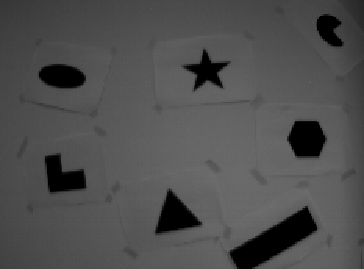
\includegraphics[width=\textwidth]{dvs1}
         \caption{}
         \label{fig:dvs1}
     \end{subfigure}
     \hfill
     \begin{subfigure}[b]{0.4\textwidth}
         \centering
         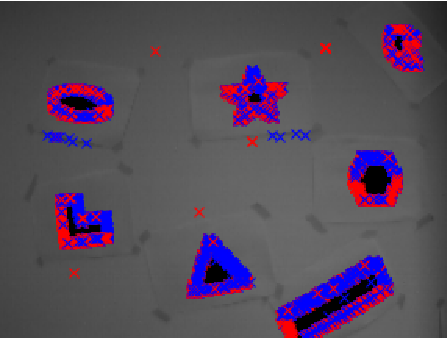
\includegraphics[width=\textwidth]{dvs2}
         \caption{}
         \label{fig:dvs2}
     \end{subfigure}
    \caption[Example data recorded from a DVS camera]{This dataset involves moving a DVS camera around a collection of shapes. The camera has slightly moved between the frame shown in (a) and the frame shown in (b). The corresponding changes in pixel lighting are shown in (b). Pixels which have gotten brighter are marked with red, and pixels which have darkened are shown in blue \cite{spiking_shapes}}
    \label{fig:dvs_ex}
\end{figure}

% Another popular sensor is the "silicon cochlea." Inspired by the real cochlea, there are 64 channels that produce events in response to sound of different frequencies \citep{silicon_cochlea}.

%********************************************************************%

\section{Converting ANNs}

Many researchers seek the benefits of SNNs but also want to avoid training them. This has sparked research into converting trained ANNs into SNNs. The main advantage of this approach is that one does not have to work around the non-differentiability of the spiking activation function and can simply train a model with standard deep learning techniques.

\citet{convert_no_bias} are credited with developing early conversion techniques for fully connected networks. Now, almost any existing neural network layer can be converted to a spiking equivalent, including convolution and softmax layers \citep{convert_with_bias}. These converted models may have slightly higher error rates but can offer about a 2x reduction in the number of operations when compared to the original ANNs.

This thesis, however, aims to train SNNs rather than convert them. We take this approach because converted SNNs typically require neurons to have high spiking frequencies and as a result consume more power, reducing the benefits of using SNNs in the first place. Additionally, we aim to explore event-based data in a biologically plausible setting. Converted models are typically trained on data with events calculated after the fact and perform poorly when fed more realistic spiking data from a DVS sensor.

% Performance of these two learning techniques?
We also leave the door open to use more biologically inspired, unsupervised learning techniques to train our models in the future. In particular, spike timing dependent plasticity (STDP), or Hebbian learning, has shown great promise \citep{KHERADPISHEH201856}. Winner-take-all (WTA) circuits that make use of inhibition are also very interesting.

%********************************************************************%

\section{SNNs and Computer Vision}

Many computer vision tasks are being solved with SNNs. MNIST remains a popular benchmark \citep{10.3389/fncom.2015.00099}, but SNNs also perform well on more complex datasets such as ImageNet. \citet{10.3389/fnins.2019.00095} develop a SNN based on VGGNet and achieve a top-5 error rate of 30.04, while the state-of-the-art artificial neural network (ANN) achieves a top-5 error rate of 29.48. Other complex models such as ResNet have been trained to work directly with spiking input from a DVS camera \citep{resnet_events}.

% explain classification in SNNs and why regression is hard
Most computer vision research with SNNs to date has chosen to work with classification problems. It is stated in many papers that classification problems are easier to apply SNNs to than regression problems. This is due to the fact that there is consensus on how to interpret spike trains to classify an input (method shown in Figure~\ref{fig:snn_classifier}), but there are many choices in how to interpret spike trains to represent continuous valued outputs. The only published work on regressions with SNNs is \citet{regression_steering}. The model in that paper, however, was converted from a trained ANN. We train our SNN from scratch and offer an alternative method to creating an output layer for a regression problem.

\begin{figure}
    \centering
    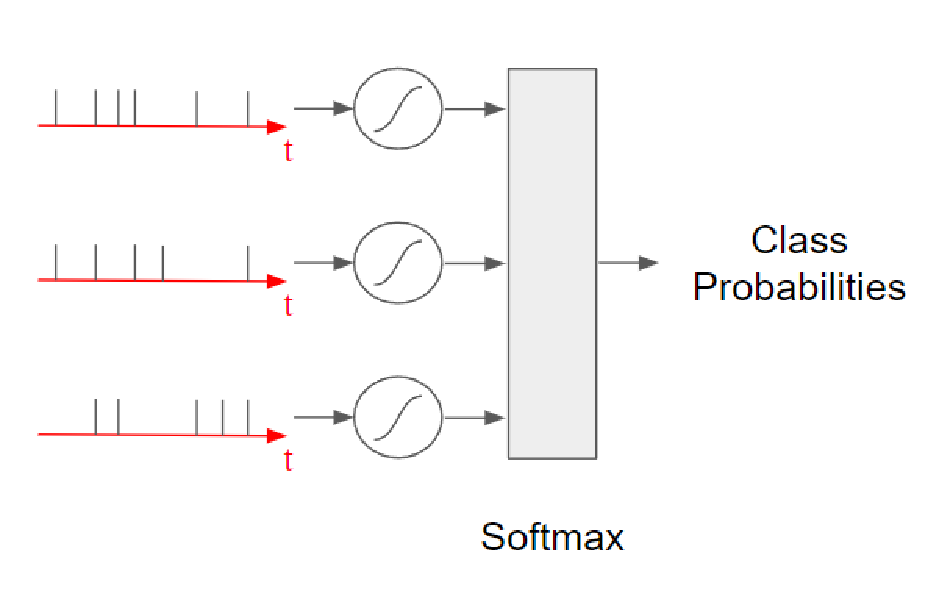
\includegraphics[width=0.6\textwidth]{snn_classifier}
    \caption[Interpreting spike trains to classify inputs]{An example on how spike trains can be interpreted for a classification task. Here, each spike train is integrated to count how many spikes there have been in a time interval. These counts are then passed to a softmax layer. Each neuron is assigned to a possible class, and the predicted label is taken from the neuron with the most spikes. }
    \label{fig:snn_classifier}
\end{figure}

Our eye model has an unstructured input, whereas pixels in images from datasets such as MNIST and CIFAR-10 follow a structured arrangement. Permutation invariant MNIST, or PI-MNIST \cite{le2015simple}, is an interesting benchmark that changes the arrangement of pixels so that standard convolution layers cannot be used to classify digits. This is the only benchmark that remotely resembles the unstructured input of the retina in this thesis.

%%%%%%%%%%%%%%%%%%%%%%%%%%%%%%%%%%%%%%%%%%%%%%%%%%%%%%%%%%%%%%%%%%%%%%

\chapter{The Task}

Our goal is to create an SNN that, when used, allows the biomimetic eye to track an object through space. The object of choice is a white ball that moves against a background whose color varies in different shades of grey. The biomimetic eye of \citet{Arjun} has four main parts, one of which we control with a SNN. We test our implementation by checking that our modified eye model performs certain movements with biological accuracy and that it can successfully track the target. In this section we provide more detail about the eye model, focusing on the retina and foveation controller that our work replaces with a SNN.

%********************************************************************%

\section{Retina}

Our virtual retina, like a real one, sits at the back of the eye and contains photoreceptors that receive input from the scene. We work with color input, so each photoreceptor collects a red, green, and blue color value. The photoreceptors are distributed according to a log-polar distribution whose equation is shown below. This distribution puts most of the photoreceptors in the center of the retina, simulating the fovea which allows for high acuity vision in the center of mammalian fields of view.

$$
d_k = e^{\rho_j} 
    \begin{bmatrix} 
        \cos( \alpha_i) \\ 
        \sin( \alpha_i) 
    \end{bmatrix}
    +
    \begin{bmatrix} 
        \mathcal{N}(\mu, \sigma^2) \\ 
        \mathcal{N}(\mu, \sigma^2)
    \end{bmatrix},
    \text{ for }
    1 \leq k \leq \text{14,400}
$$

% cite papers about actual eye structure

We choose to work with 14,400 photoreceptors, incrementing $\rho_j$ and $\alpha_i$ in steps of 1 with the conditions: $ 0 \leq \rho_j \leq 40 $ and $ 0 \leq \alpha_i \leq 360 $. The second term of the equation is additive noise picked IID from a Gaussian distribution with mean $ \mu = 0 $ and variance $ \sigma^2 = 0.0025 $. A visual of this distribution can be seen in Figure~\ref{fig:task_log_polar_retina}. Having a lower amount of photoreceptors speeds up simulation and training, but the number can be scaled up as human retinas have about about 6 million cones (for color) and 120 million rods (for black and white) \citep{rodsAndCones}. 

\begin{figure}
    \centering
    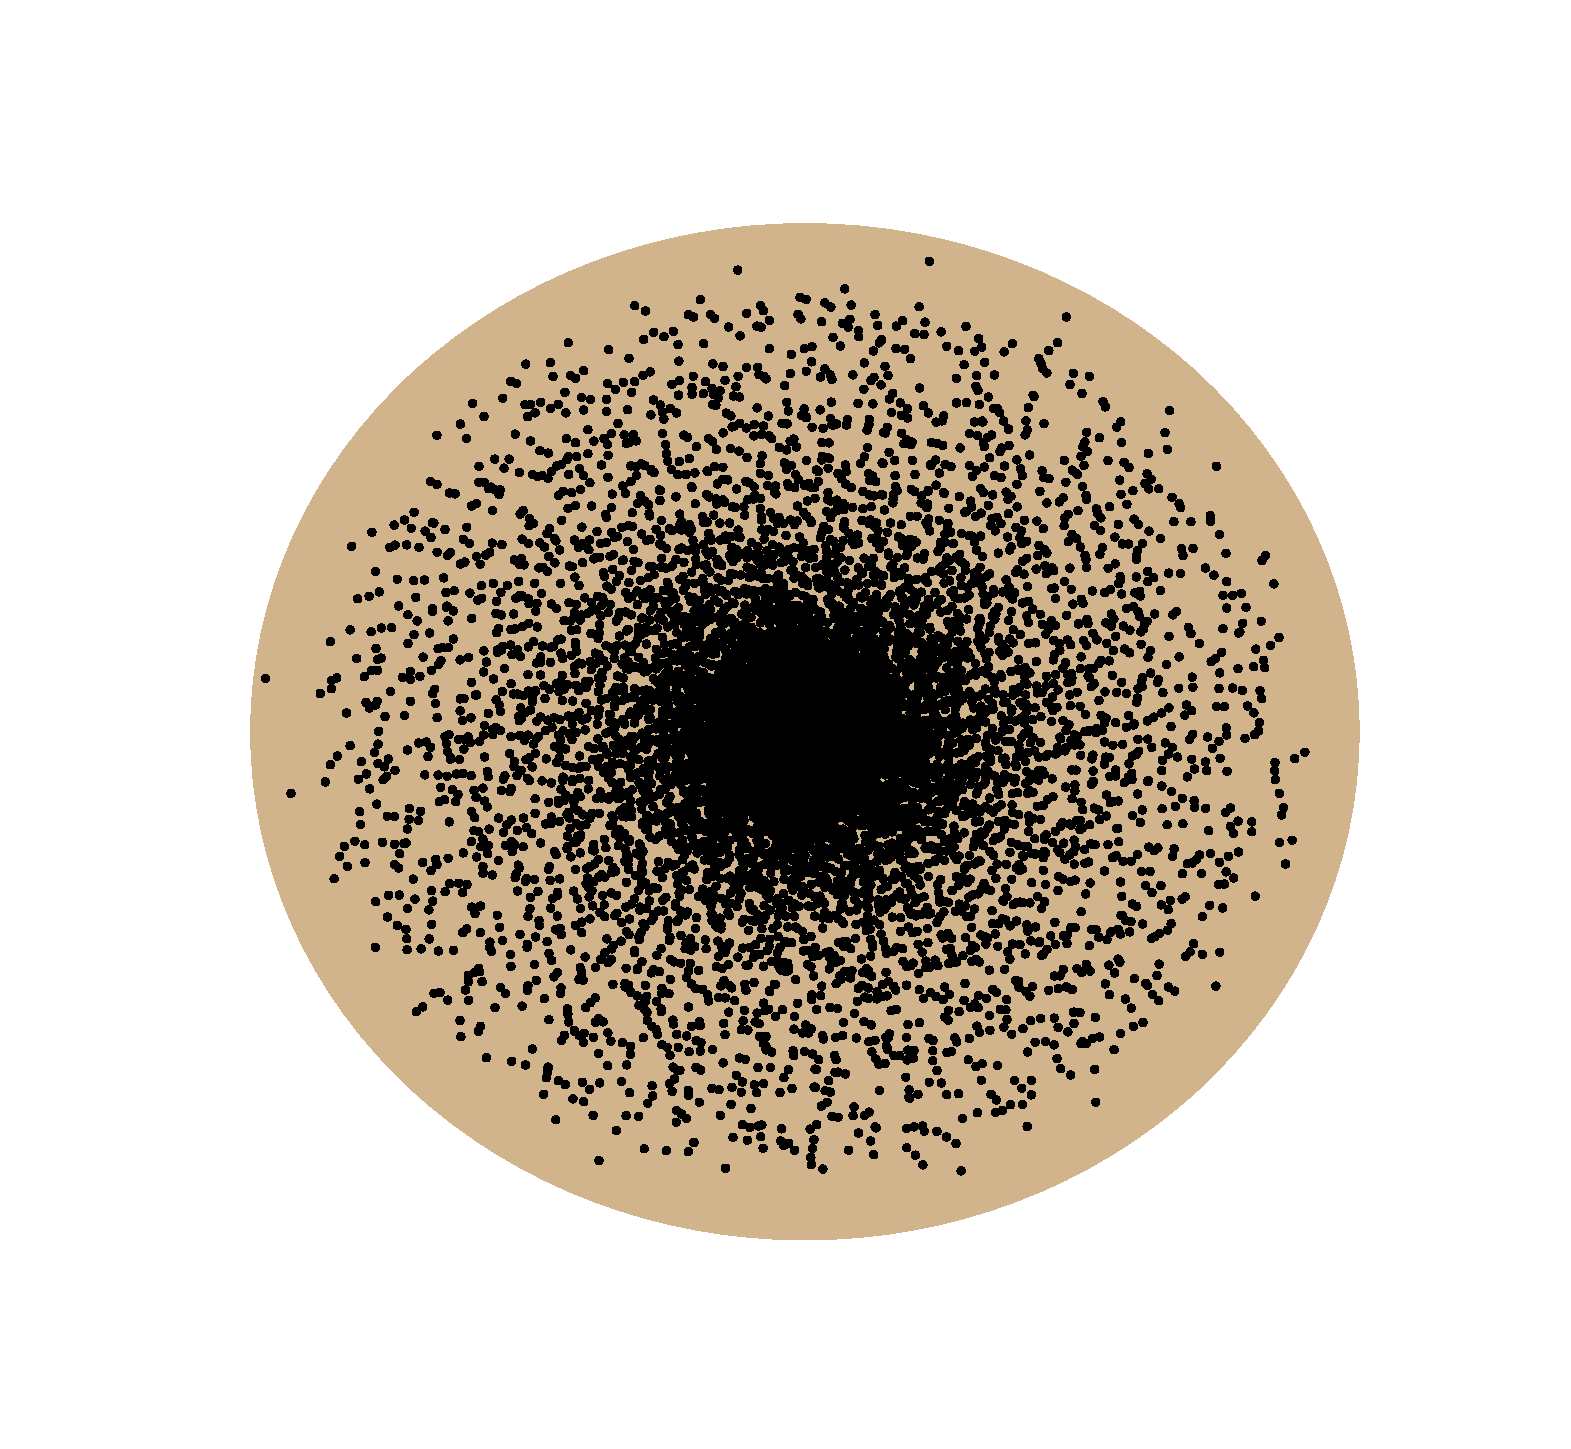
\includegraphics[width=0.6\textwidth]{retina_log_polar}
    \caption[Photoreceptor distribution on the retina]{The photoreceptors of the retina arranged according to a noisy log-polar distribution. The 2D distribution is mapped to the spherical back of the eyeball when ray casting.}
    \label{fig:task_log_polar_retina}
\end{figure}

In our simulation, rays are traced from the retina, through the pupil and lens, to see if they intersect with objects in the scene. These intersections tell us what color will be seen at a given photoreceptor, resulting in 14,400 RGB values. We stack each color channel vertically to create a vector, referred to as the optic nerve vector (ONV), of dimension 43,200.

%********************************************************************%

\section{Ocular Organs and Muscles}

The other parts of the eye model include the lens, pupil, and 6 extraocular contractile (EOC) muscles. The pupil and lens help to focus our target onto the retina while the EOC muscles create the movement required for the eye to track the target. Each of these systems is simulated with inverse dynamics control in this thesis; more detail about each subsystem is provided in Appendix \ref{appendix:eye}.

%********************************************************************%

\section{Neural Network Controllers}

For added realism and biological performance, each of the ocular organs and muscles can also be controlled with their own neural network. A summary of the whole system is shown in Figure~\ref{fig:eye controller summary}. The pupil and lens are each controlled with a shallow neural network that takes the ONV as input and outputs one value for the muscle activation.

EOC muscle control is split up into two parts. First the ONV is input to the foveation controller, which outputs 2 values $\theta$ and $\phi$. These two values represent the change in the horizontal and vertical directions relative to the eye's current gaze direction. An example of the target moving is pictured in Figure~\ref{fig:ball_movement}. The foveation controller is implemented as a locally connected network, dubbed a LiNet. The details of how a LiNet works can be found in Appendix \ref{appendix:linet}. The muscle controller then takes these two angles and outputs an activation for each of the EOC muscles to perform the movement.

% \begin{figure}
%     \centering
%     \includegraphics[width=0.5\textwidth]{eye_coordinates.png}
%     \caption{The two angles $\theta$ and $\phi$ needed to describe how the eye must move to follow the target.}
%     \label{fig:2D eye coordinates}
% \end{figure}

\begin{figure}
     \centering
     \begin{subfigure}[b]{0.48\textwidth}
         \centering
         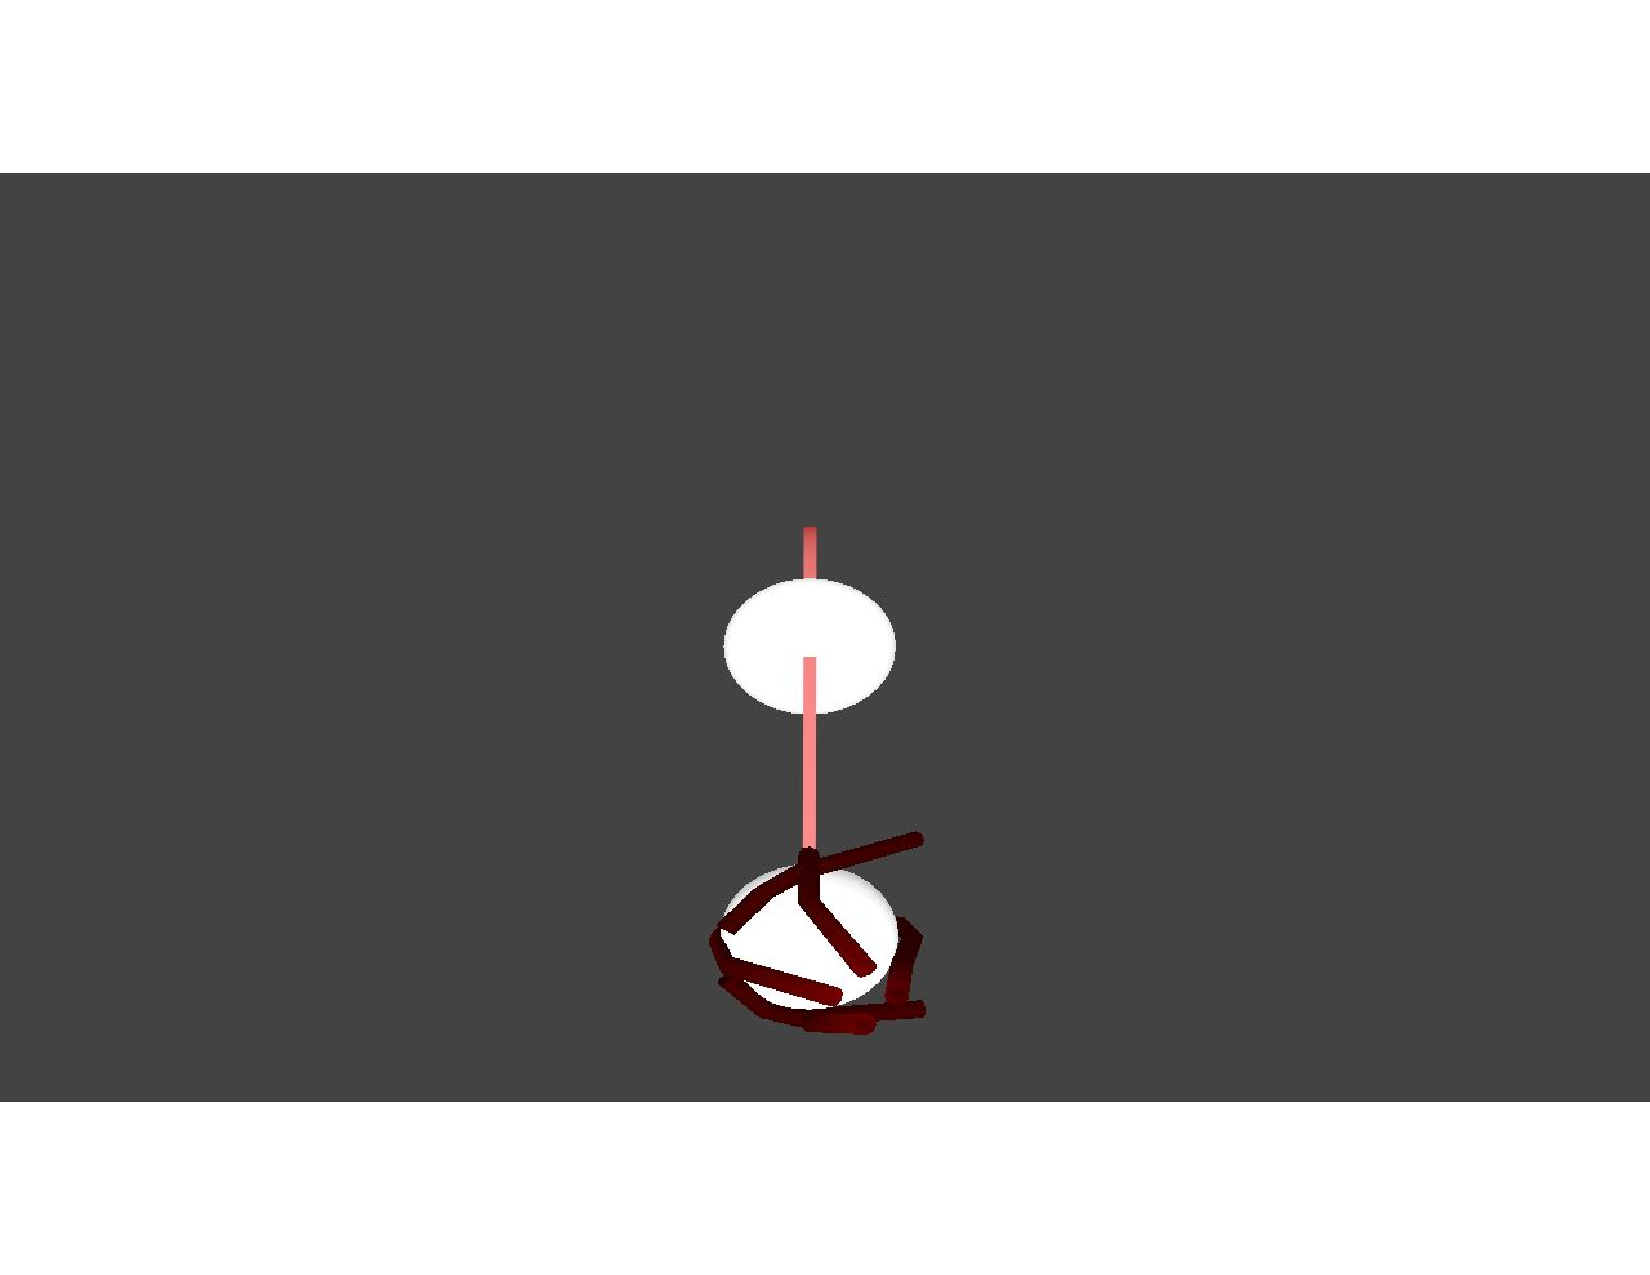
\includegraphics[width=\textwidth]{image000028}
         \caption{}
         \label{fig:ball_pos1}
     \end{subfigure}
     \hfill
     \begin{subfigure}[b]{0.48\textwidth}
         \centering
         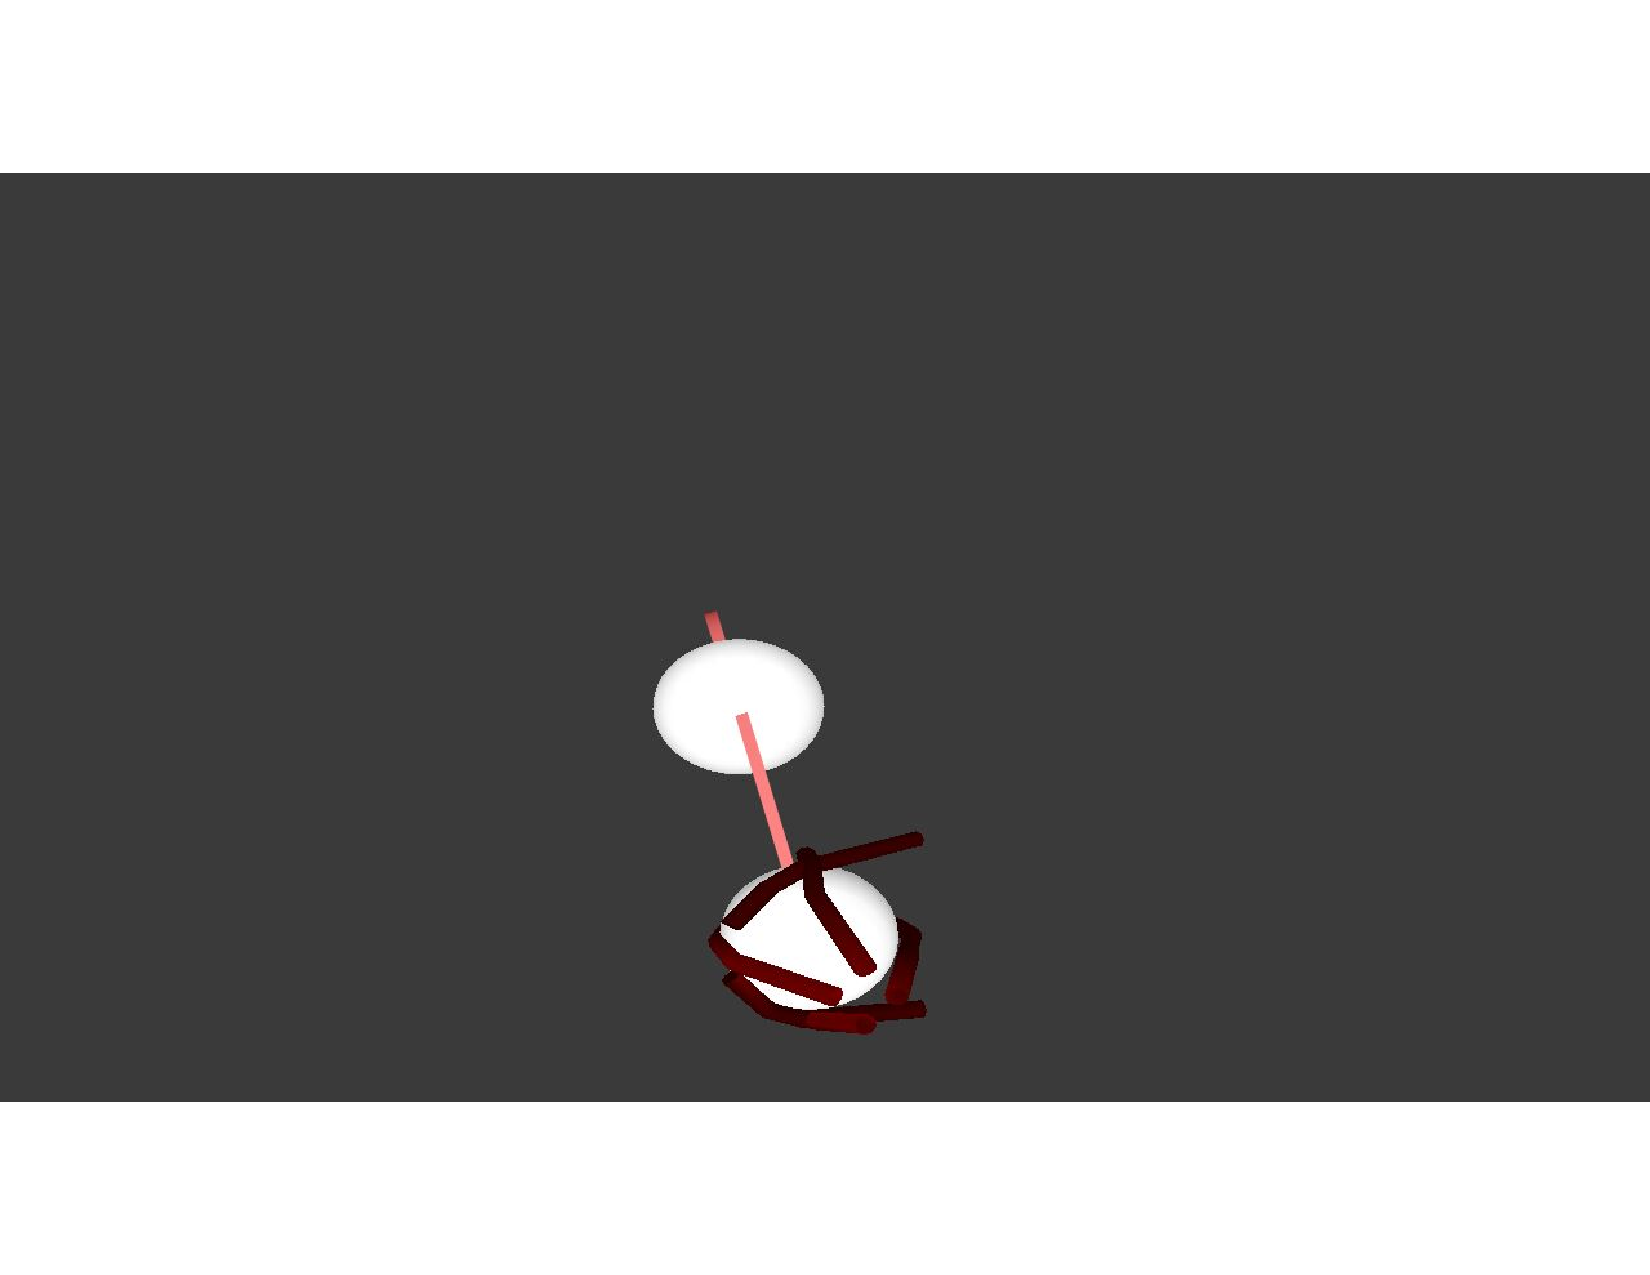
\includegraphics[width=\textwidth]{image000068}
         \caption{}
         \label{fig:ball_pos2}
     \end{subfigure}
    \caption[Target movement and corresponding gaze correction]{The ball moves from one point (a) to another (b). The red line reveals the current gaze direction, which shifts to the left and slightly downward between the two frames. This movement is encoded in the angles $\theta$ and $\phi$.}
    \label{fig:ball_movement}
\end{figure}


% add red box
\begin{figure}
    \centering
    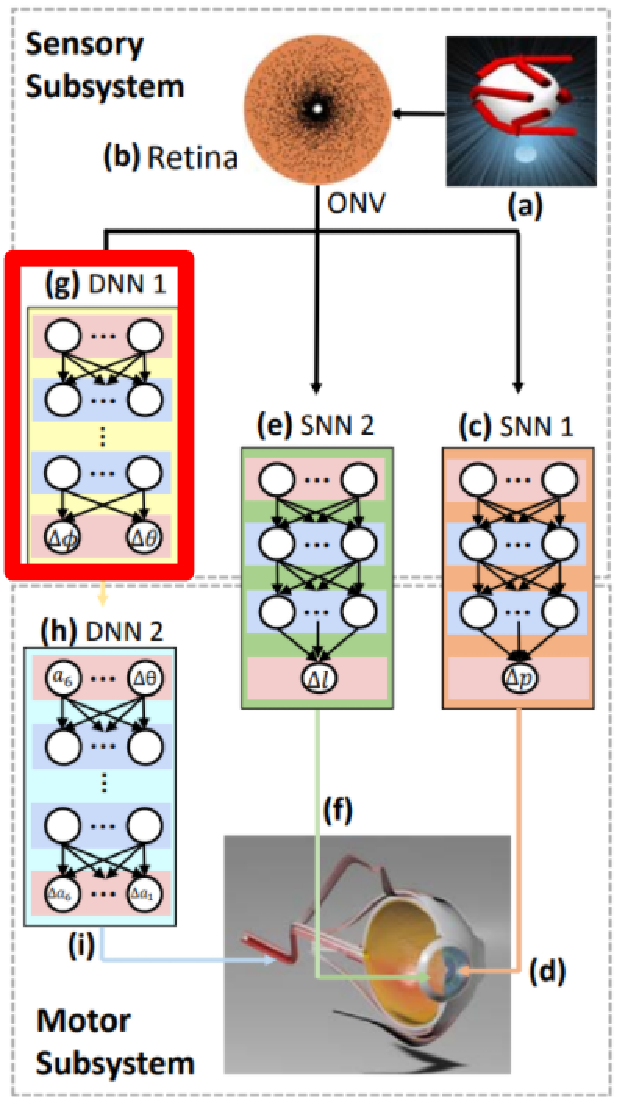
\includegraphics[width=0.5\textwidth]{subsystem_summary2}
    \caption[Summary of existing oculomotor system controlled by neural networks]{Summary of the eye's neural network controller system. The foveation controller, which we replace with a SNN, is highlighted with the red box. Note that SNN in this figure stands for ``shallow neural network'', not spiking neural network. DNN stands for ``deep neural network.'' Figure from \citep{Arjun}. }
    \label{fig:eye controller summary}
\end{figure}

%********************************************************************%

\section{Eye Movements}

We test our SNN foveation controller with the framework created by \citet{Arjun}. This involves moving the target in three different ways and noting if the eye can successfully track it. The movements are defined below.

\begin{enumerate}
    \item \textit{Fixation}: The eye maintains focus on the target while it stays in place. The eye itself looks still and stable but may have small oscillations. We test that these small oscillations exist as they add to the biological plausibility of the model. 
    \item \textit{Saccade}: A quick eye movement to bring a visual target from peripheral vision to the center of the retina. We test that our SNN model matches the angular orientation, velocity, and acceleration of a real eye.
    \item \textit{Smooth pursuit}: Once a moving visual target is fixated, the eye can pursue the target as it moves. The trajectory of the eye movement is not entirely smooth but includes random oscillation. We track the orientation of the eye through time to make sure that it successfully follows the target. Good performance here is an indication that the eye can track the target through many different trajectories.
    % \item \textit{Projectile Motion}: This is similar to smooth pursuit except that the target now changes size as it moves away from the eye. 

% We also quantitatively evaluate how well our SNN performs compared to the LiNet.

\end{enumerate}

%%%%%%%%%%%%%%%%%%%%%%%%%%%%%%%%%%%%%%%%%%%%%%%%%%%%%%%%%%%%%%%%%%%%%%

\chapter{Spiking Neurons}

In this chapter we introduce the basics of spiking neural networks.

We first define the popular artificial neuron model currently in use. In a network with L layers, $W^l, l \in {1, ..., L}$ is the weight matrix connecting layer $l-1$ to layer $l$. We multiply the output of the previous layer, $x^{l-1}$, with $W^l$, add biases $b^l$ to the result, and finally apply the ReLU activation. This artificial neuron model is summarized in Figure~\ref{fig:neuron_ann}, with the equations given below.

% , and number of neurons in a layer is $M^l$
% $$ a_i^l = max(0, \sum_{j=1}^{M^{l-1}} W_ij^l a_j^l-1 + b_i^l ) $$

$$ a^l =  W^l x^{l-1} + b^l $$
$$ x^l = max(0, a^l) $$

% Image of ANN neuron
\begin{figure}
    \centering
    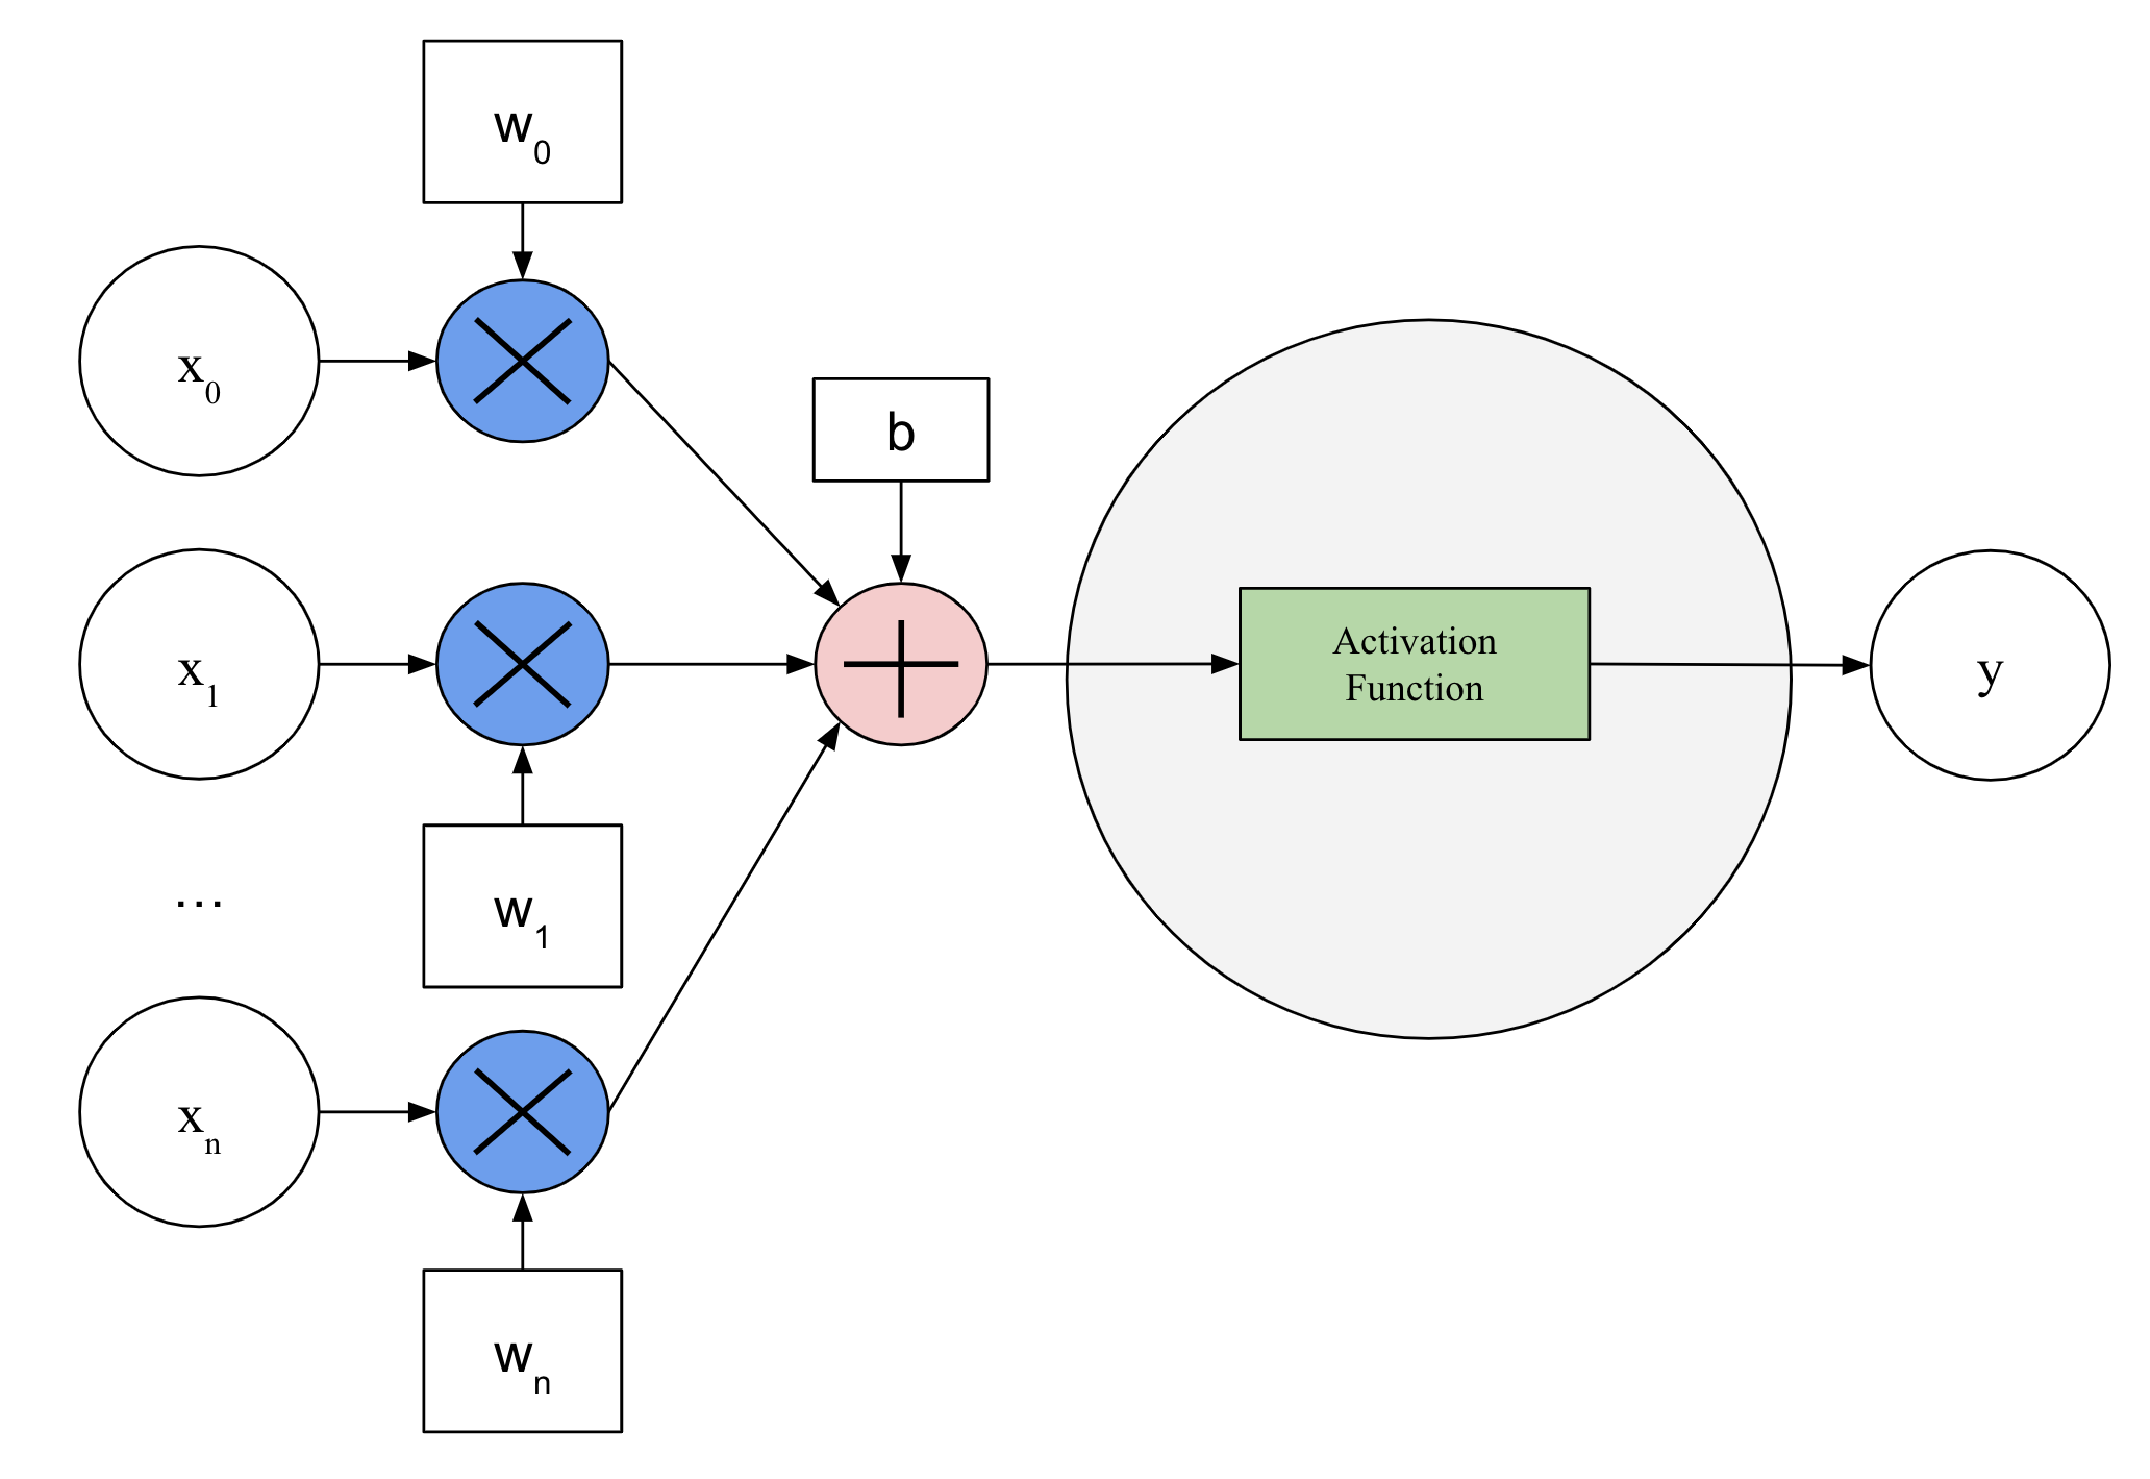
\includegraphics[width=\textwidth]{neuron_ann}
    \caption[Artificial neuron model]{How a traditional artificial neuron operates.}
    \label{fig:neuron_ann}
\end{figure}

Before moving on to a spiking neuron, we define some terms. A synapse refers to the connection between two neurons and has an associated weight value that is tuned during training. If we are looking at a specific neuron, all neurons in the previous layer that are connected to it are presynaptic neurons and all neurons connected to it in the next layer are postsynaptic neurons. The inputs are time varying and in the form of spike trains, which are sequences of 1's and 0's. All spike trains in the network are the same length, which is treated as a hyperparameter.

Each spiking neuron maintains a state variable known as membrane voltage, which we call $U$. If a presynaptic neuron spikes, we add the corresponding synapse weight to this membrane voltage. We store the weights in a matrix $W$, and the presynaptic outputs are stored in a tensor $X$. If no spikes are input to the neuron, the membrane voltage decays exponentially. This decay is controlled with the hyperparameter $\beta$. If $U$ crosses a certain threshold $U_\text{thr}$, then the neuron outputs a spike and resets $U$ to zero. This spiking behavior is captured by the Heaviside step function, represented by $\Theta$ and shown in Figure~\ref{fig:surrogate_grad}. The spiking neuron is summarized in Figure~\ref{fig:neuron_snn}.

% Image of SNN neuron
\begin{figure}
    \centering
    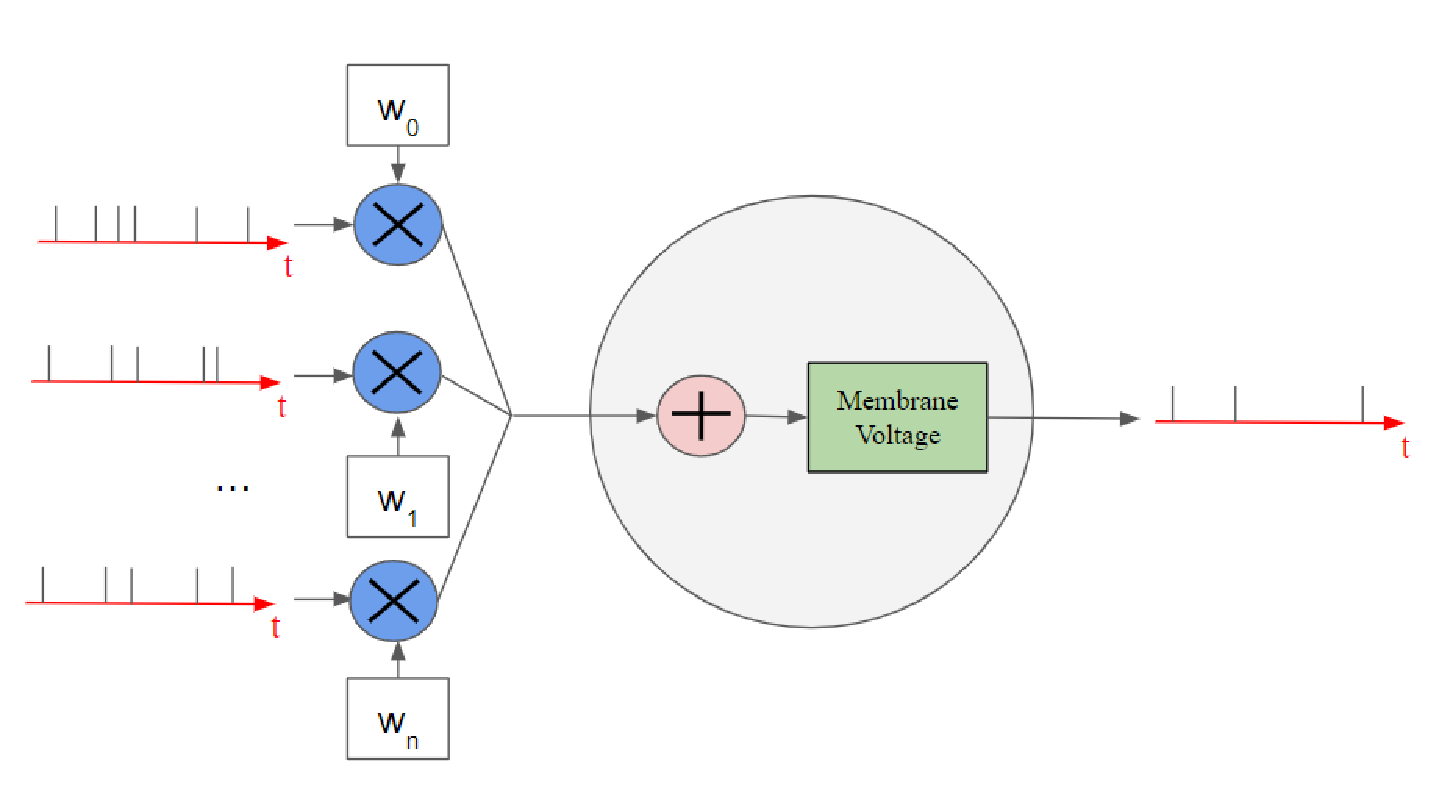
\includegraphics[width=\textwidth]{neuron_snn}
    \caption[Spiking neuron model]{How a spiking neuron operates.}
    \label{fig:neuron_snn}
\end{figure}

From the two equations below, $U(t)$ used for calculating the membrane voltage of a neuron at timestep $t+1$ and $S(t)$ is the spiking activation function. The membrane voltage equation is used by the Python package snnTorch \citep{snnTorch}, which is what we used for the work of this thesis. This neuron model is known as the leaky integrate-and-fire (LIF) neuron, named because it ``leaks'' voltage in the absence of input. We show an example of a LIF neuron in Figure~\ref{fig:lif_spike_example}. 

$$ U(t) = \underbrace{\beta U(t-1)}_{\text{decay}}
+ \underbrace{W X(t)}_{\text{input}}
- \underbrace{S(t-1)U_\text{thr}}_{\text{reset}} 
$$

$$
S(t) = \begin{cases} 
      1 & \text{if } U(t) > U_\text{thr} \\
      0 & \text{otherwise }
      \end{cases}
      = \Theta (U(t) - U_\text{thr})
$$

% Image of input spikes, corresponding voltage increasing and decaying, and output spikes
\begin{figure}
    \centering
    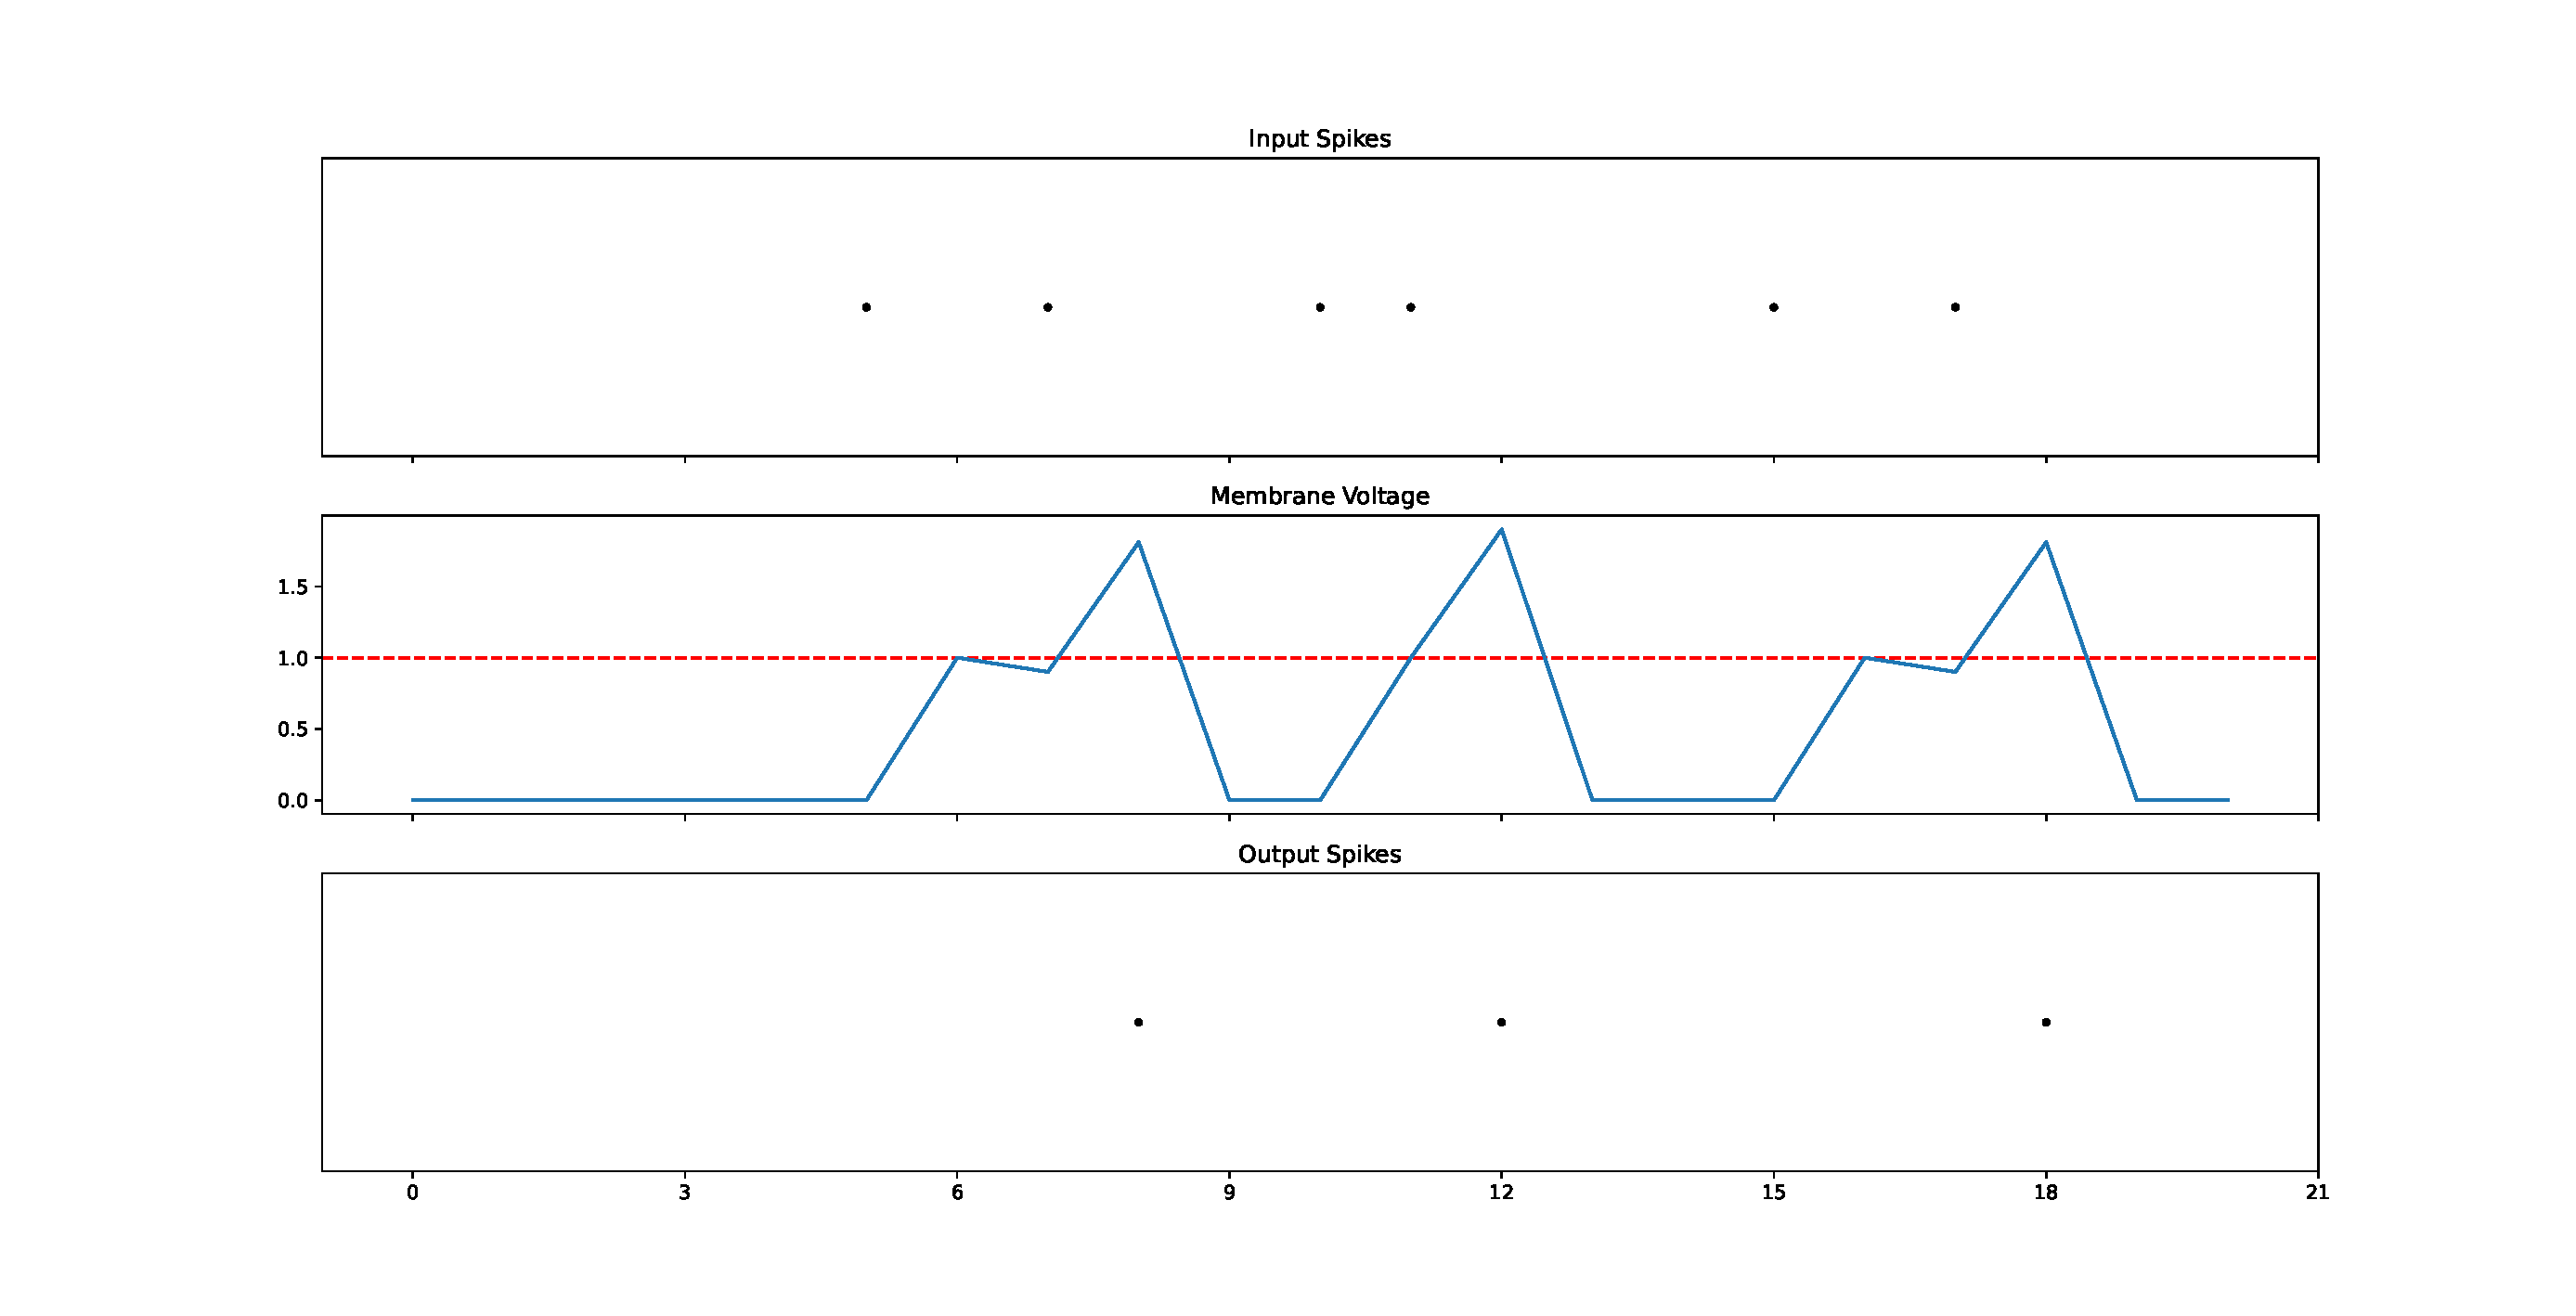
\includegraphics[width=\textwidth]{snn_spike_example}
    \caption[Leaky Integrate-and-Fire (LIF) neuron membrane voltage demonstration]{Demonstration of a LIF neuron. Input spikes to the neuron are at the top, the neuron's membrane voltage is in the middle, and output spikes are at the bottom. The threshold voltage is represented with the dashed red line. We verify that the membrane voltage increases when there is an input spike and that there is an output spike when the membrane voltage crosses the threshold. There is a reset after each output spike, represented by the steep decrease in membrane voltage. There is also a slight leak of membrane voltage in the absence of any input spikes, seen around timesteps 6 and 16.}
    \label{fig:lif_spike_example}
\end{figure}

To summarize, a SNN differs from the classic artificial neural network (ANN) in two fundamental ways. First we replace the activation function with one that only outputs 1's and 0's. Second we have inputs that vary over time. More detailed derivations of SNN theory can be found in Appendix \ref{appendix:snn}.

%********************************************************************%

\section{Outputs}

One problem associated with using SNNs is related to interpreting the output spike trains. For classification problems, the output layer has one neuron for each possible class. The output spike trains are integrated over the number of timesteps and the output label is taken from the neuron with the most spikes. Our problem, however, is a regression that involves outputting guesses for two angles. Thus far, SNN research has focused on classification as there isn't a standard way to interpret spikes into floating point values.

% figure for classification here or in related work?

To solve this problem, we utilized a linear layer to transform outputs from our SNN into our desired angles $\theta$ and $\phi$. One option would be to consolidate the output spike train somehow, such as with a sum or average, and then normalize the values. A technique that hasn't been explored much but was suggested by snnTorch was utilizing the membrane voltages of the last layer. We pass each neuron's membrane voltage at the last timestep to a linear transformation that outputs our two angles. This technique helps with backpropagation, as the network can learn what membrane voltage it should target at the end.

One thing to note is that the network outputs values at each timestep, but we take the result of the last timestep as our guessed values.

%%%%%%%%%%%%%%%%%%%%%%%%%%%%%%%%%%%%%%%%%%%%%%%%%%%%%%%%%%%%%%%%%%%%%%

\chapter{Data}

As stated before, our ONV is a vector of dimension 43,200. SNNs, however, expect inputs that vary over time. In addition, the floating point numbers that represent the light intensity at a pixel need to be meaningfully converted into ``spikes,'' or a list of 1's and 0's. This is known as converting data from the ``frame'' domain to the ``spiking'' domain, and there are two main conversion schemes that we can use to do this.

In addition to generating spiking inputs, we also introduce a ``delta'' ONV. Instead of having the eye see light intensities at the current timestep, it sees the difference between the current and previous ONV. In other words, the eye only sees what has changed in the scene, also referred to as ``event-based'' data and shown in Figure~\ref{fig:three ONVs}. Note that we have positive values if pixels get brighter and negative values if they get darker. This results in sparse input data as the eye doesn't have to keep processing what it has already seen. The delta ONV is more biologically accurate as Ganglion cells in the retina emit spikes only when there is change in the field of view \citep{eventRetina}.

\begin{figure}
    \centering
    \begin{subfigure}[b]{0.49\textwidth}
        \centering
        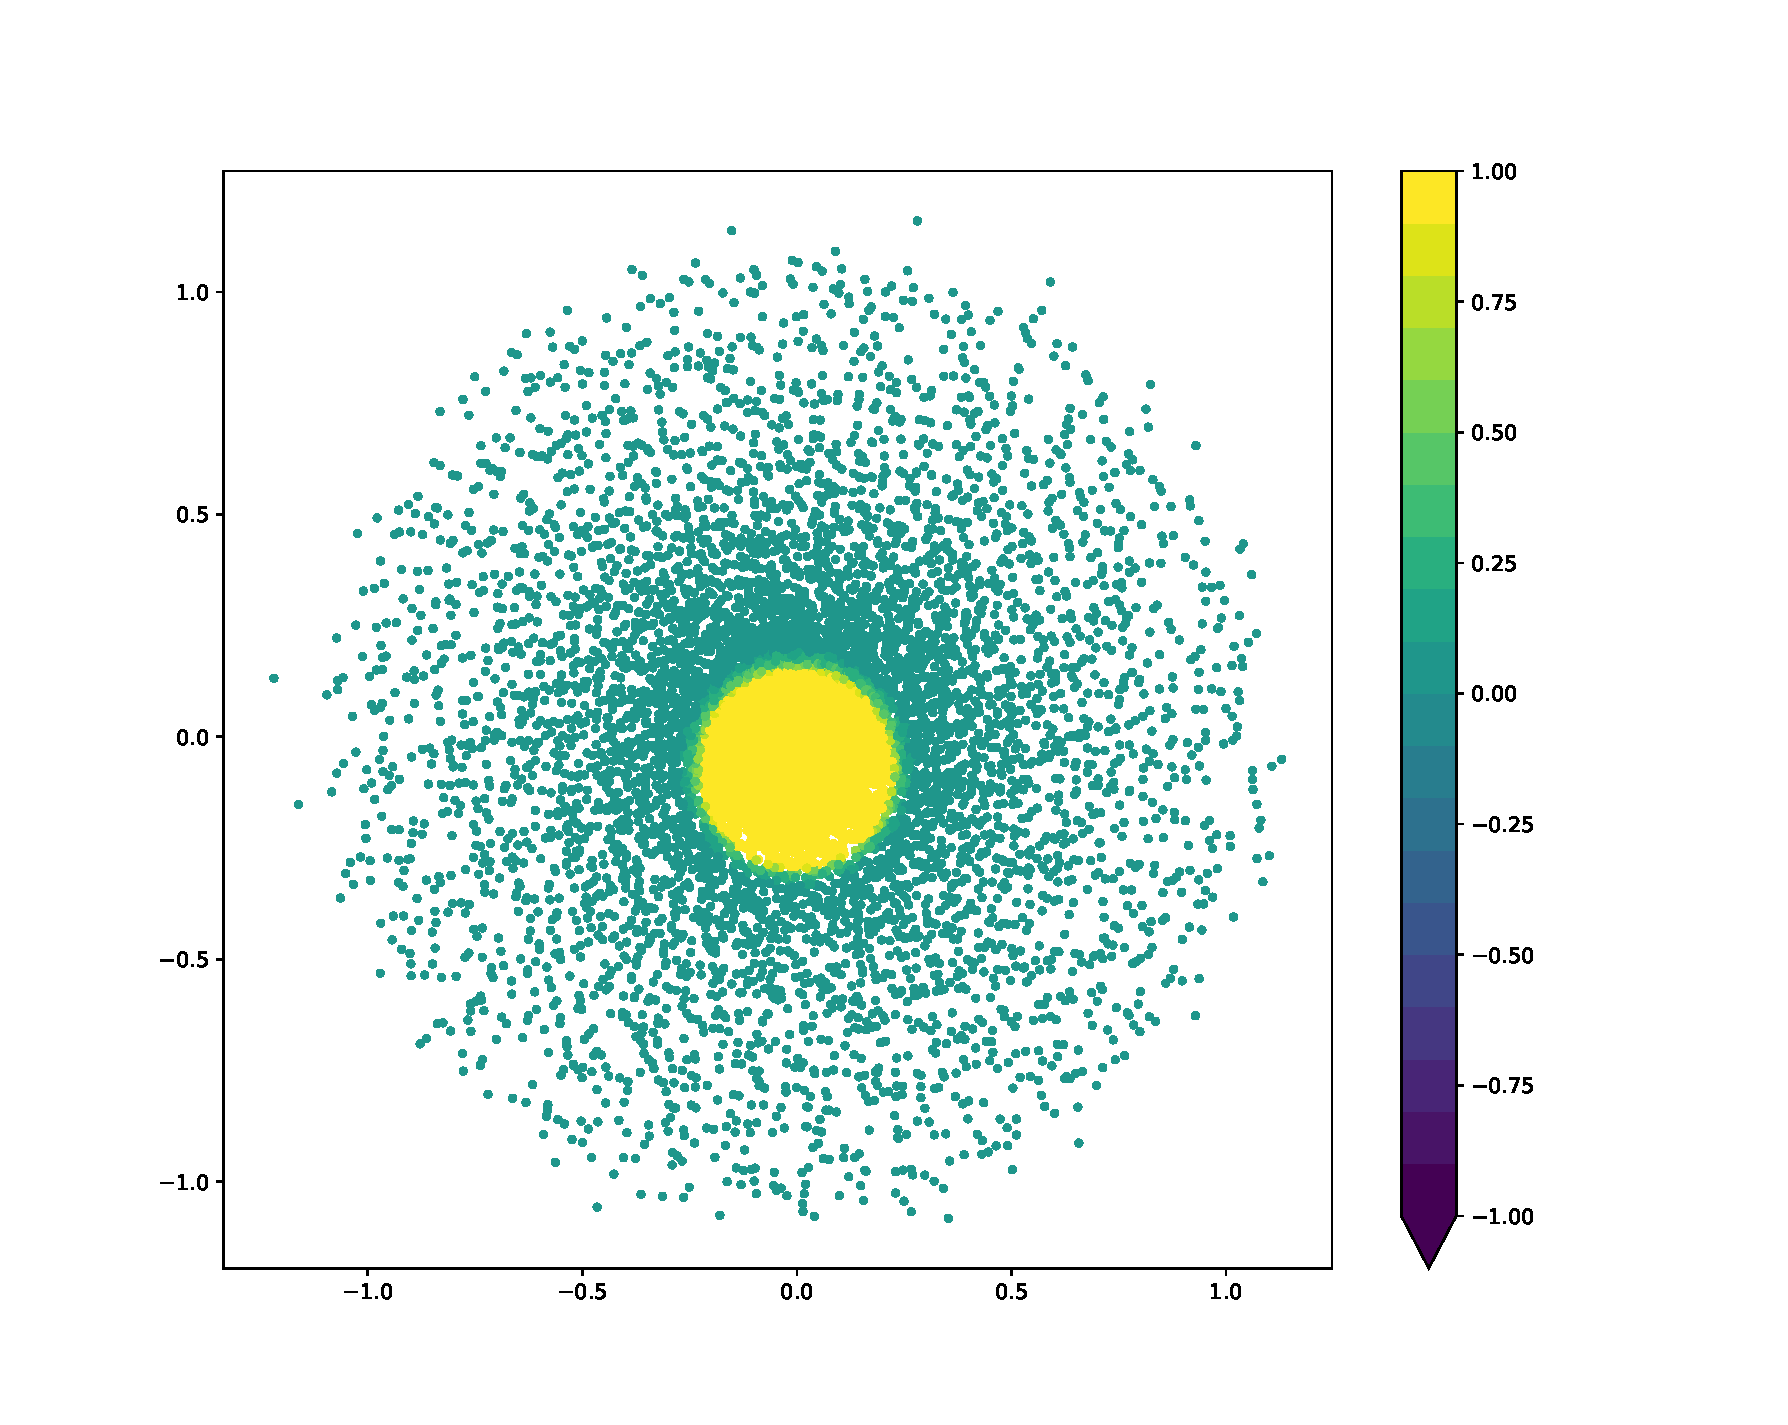
\includegraphics[width=\textwidth]{onv_normal_prev}
        \caption{Previous ONV}
        \label{fig:onv_prev}
    \end{subfigure}
    \hfill
    \begin{subfigure}[b]{0.49\textwidth}
        \centering
        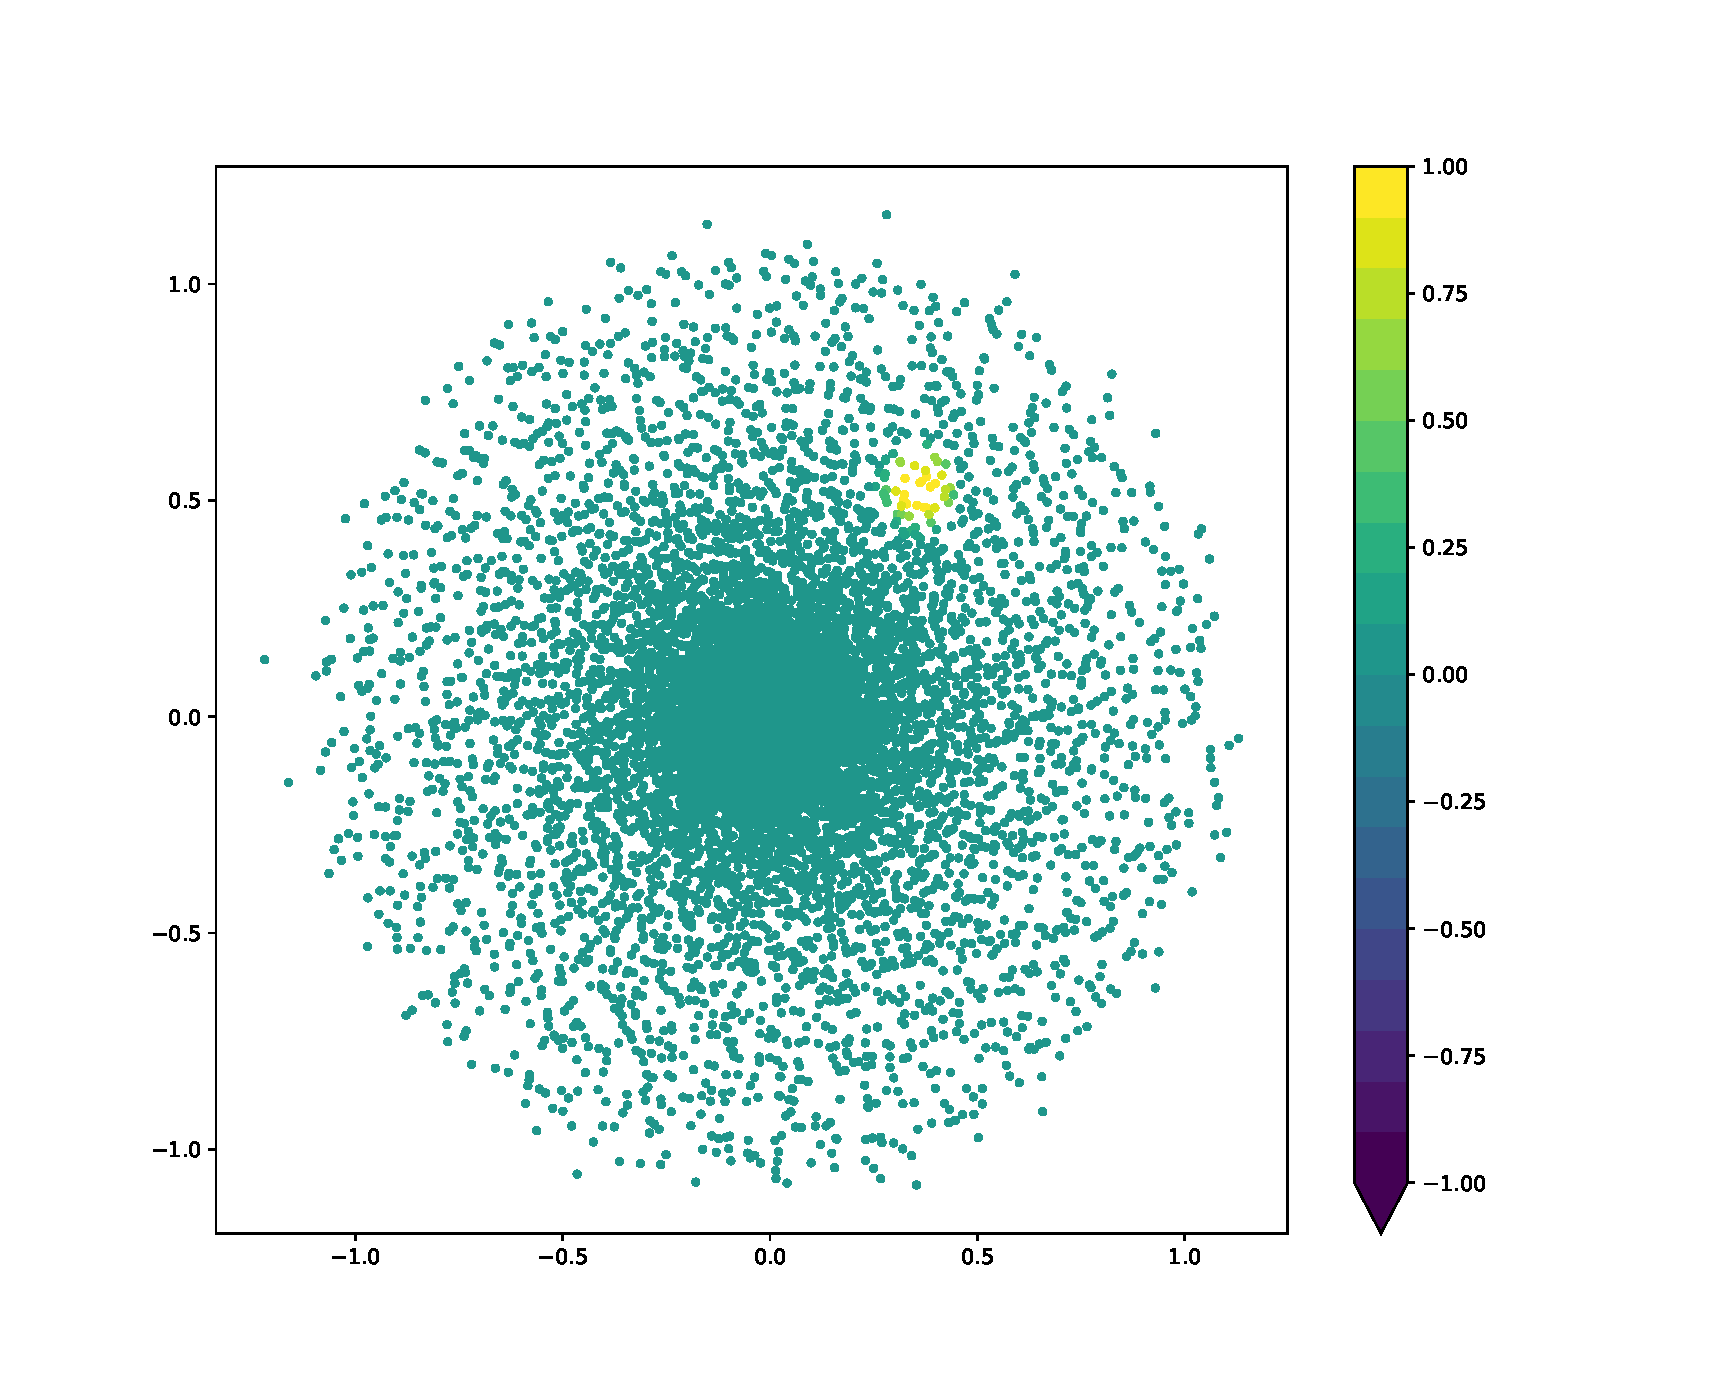
\includegraphics[width=\textwidth]{onv_normal_cur}
        \caption{Current ONV}
        \label{fig:onv_cur}
    \end{subfigure}
    \hfill
    \begin{subfigure}[b]{0.49\textwidth}
        \centering
        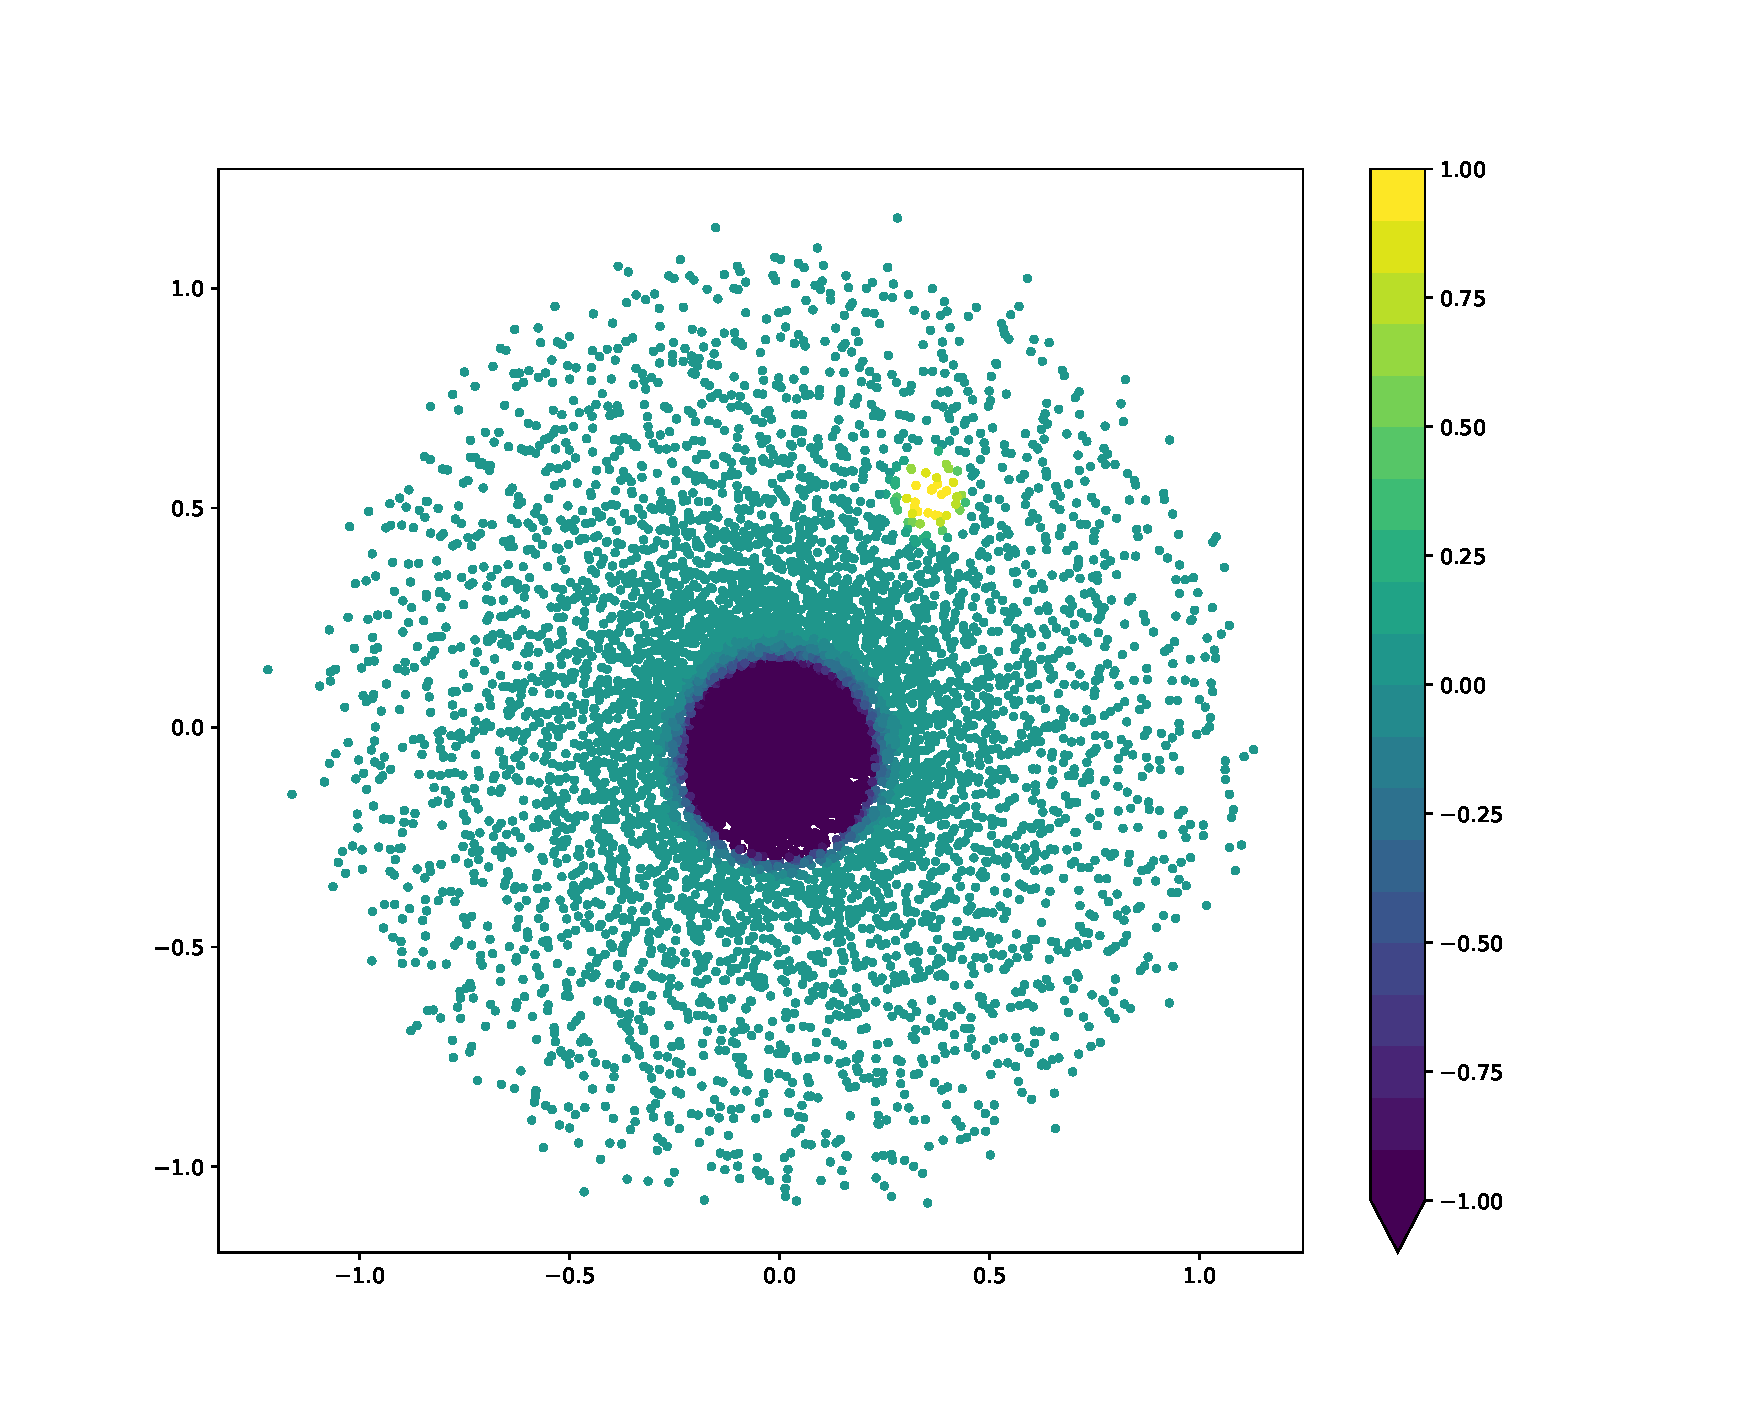
\includegraphics[width=\textwidth]{onv_delta}
        \caption{Delta ONV}
        \label{fig:onv_delta}
    \end{subfigure}
    \caption[Normal and delta ONV for a moving target]{We map ONV values collected from a scene to the photoreceptor distribution. The target has moved from one position in (a) to another in (b). (c) shows the corresponding delta ONV. The values darken where the target was in (a) and get brighter at the target's location in (b).}
    \label{fig:three ONVs}
\end{figure}

%********************************************************************%

% do I need this higher level organization?
\section{Spiking Inputs}

In this section we review the two most popular encoding methods, rate and latency encoding. It is believed that each method is used in different parts of the brain and even the visual cortex. One theory is that the retina uses rate encoding but more downstream neurons use latency encoding. We empirically found that rate encoding performed better than latency encoding on our object tracking task.

%********************************************************************%

\subsubsection{Rate Encoding}

Rate encoding attempts to encode a neuron's firing frequency. Each input value to the encoder is between 0 and 1, representing the probability that the neuron will spike at a given timestep. Then, at each timestep, we run a Bernoulli trial to see if the neuron will spike with the given probability.

For example, if our photoreceptor value was 0, the neuron would never spike. On the other hand, a value of 1 would create spikes at each timestep. A value of 0.5 would result in about half of the timesteps containing a spike. We show these examples over 20 timesteps in Figure~\ref{fig:rate_encode_3plots}.

\begin{figure}
    \centering
    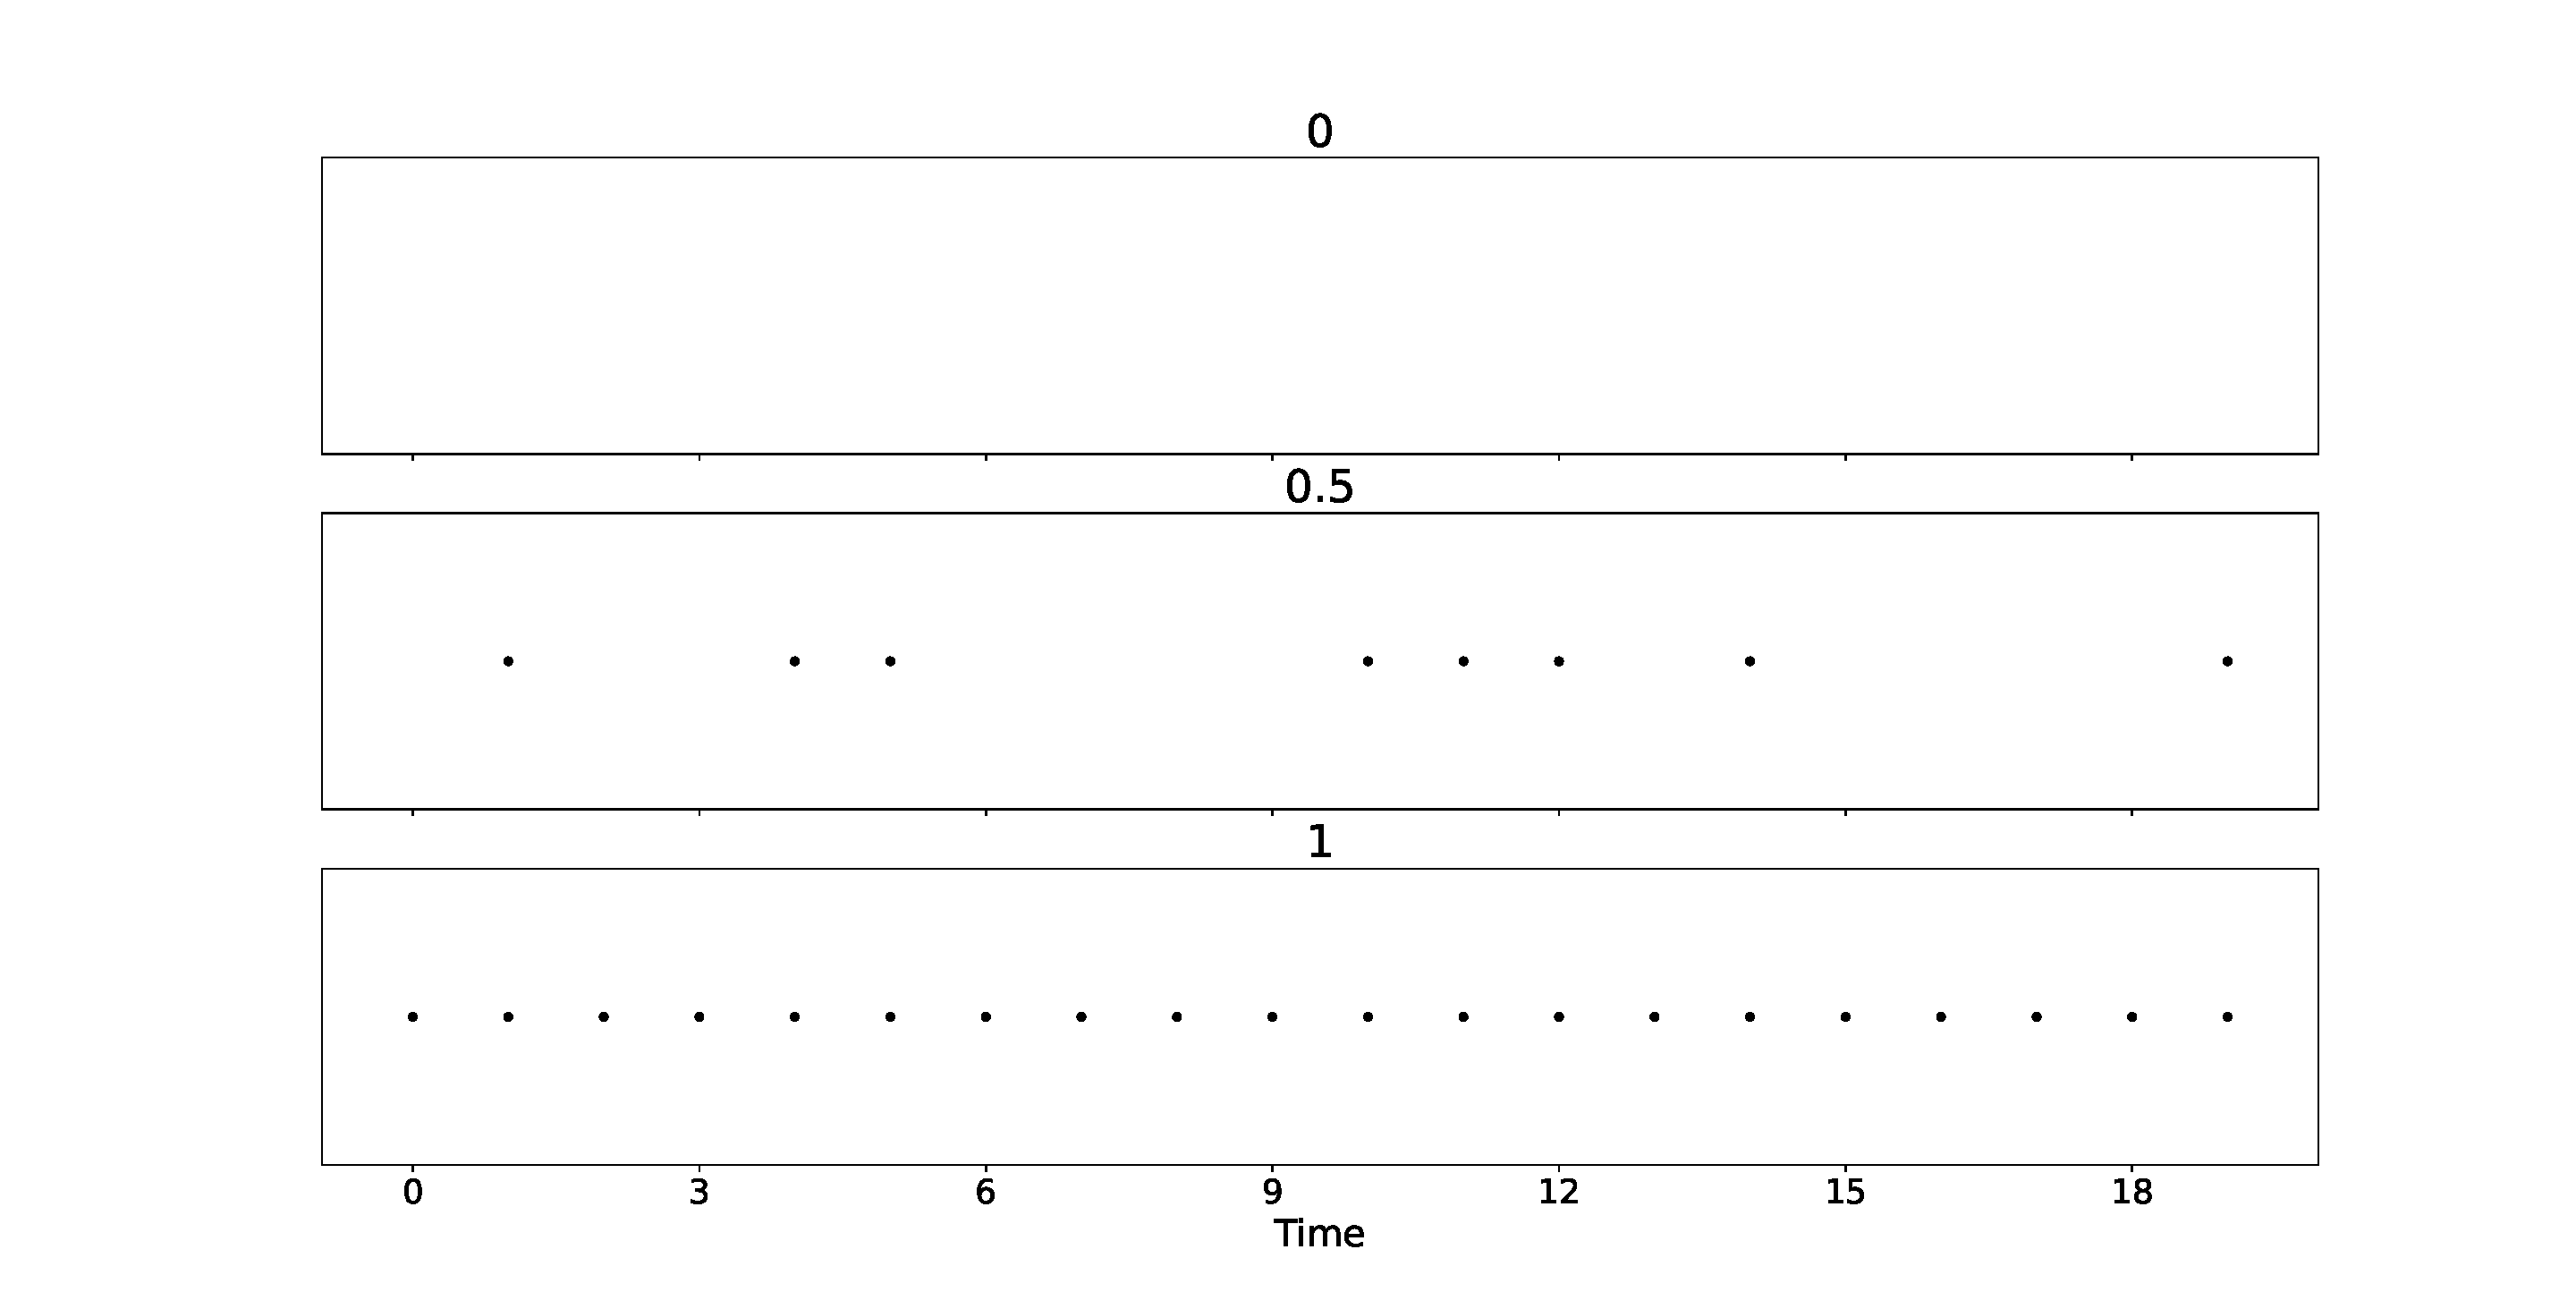
\includegraphics[width=1.0\textwidth]{neuron_3_rate}
    \caption[Rate encoding with Bernoulli trials]{Demonstration of rate encoding. From top to bottom we encode data with values of 0, 0.5, and 1.}
    \label{fig:rate_encode_3plots}
\end{figure}

\begin{figure}
    \centering
    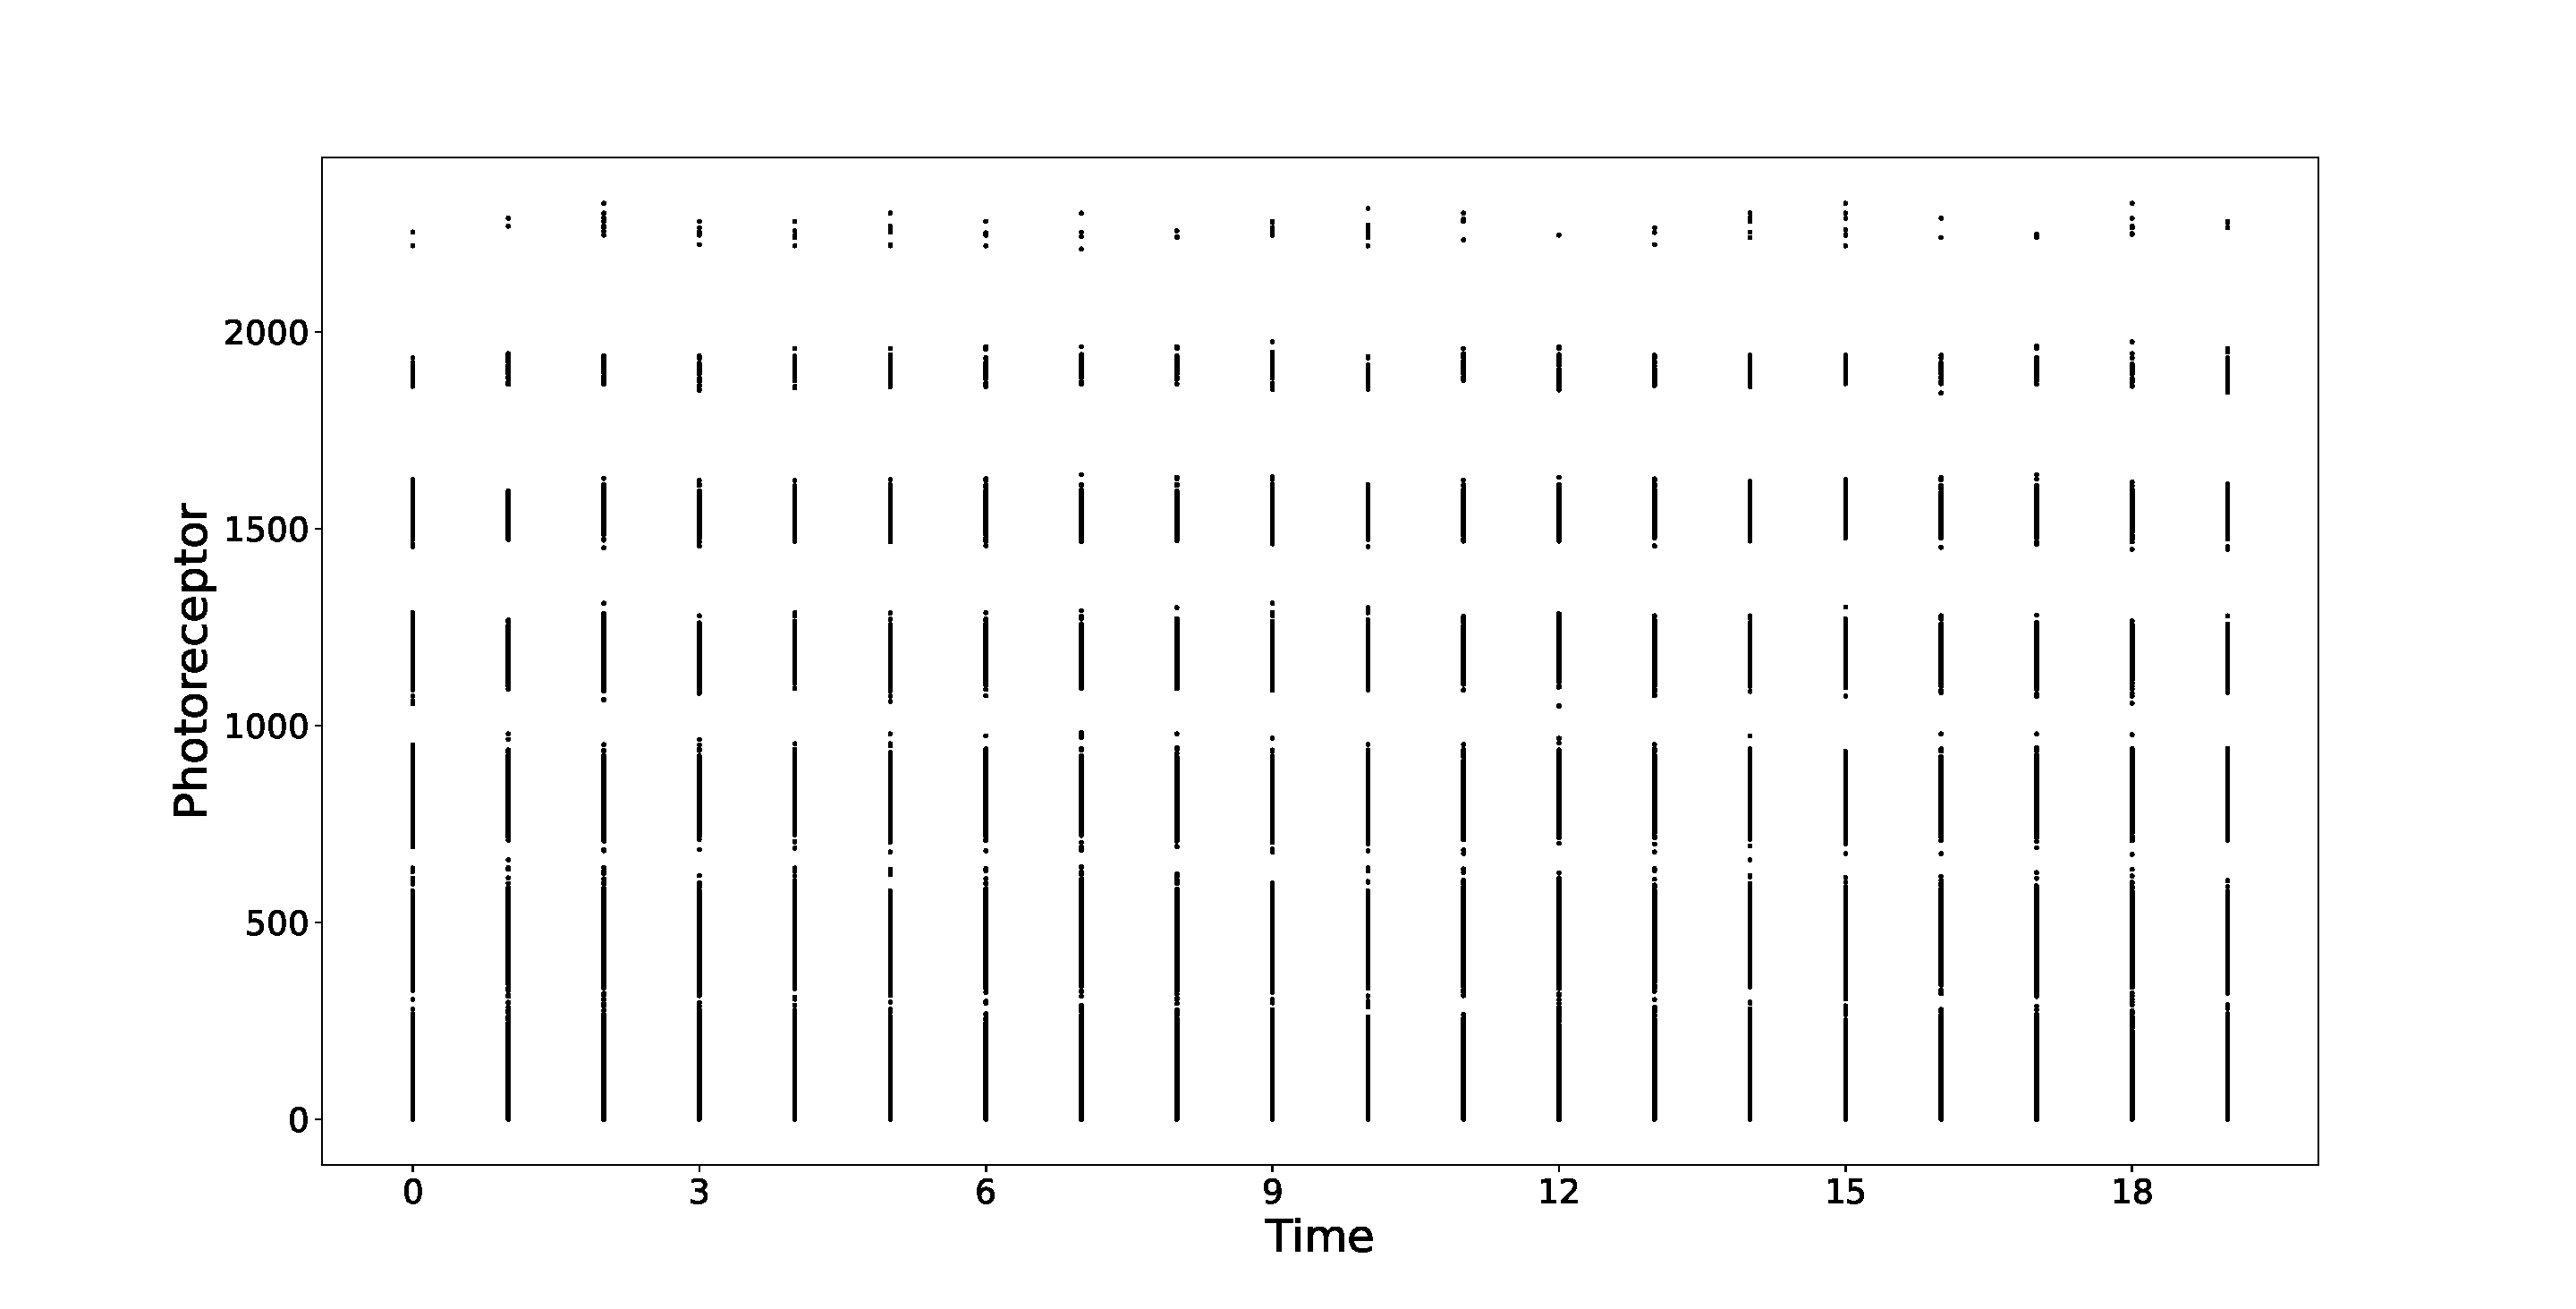
\includegraphics[width=1.0\textwidth]{onv_rate_prev}
    \caption[Rate encoded ONV]{Rate encoding of a subset of photoreceptors from the ONV in Figure~\ref{fig:onv_prev}. Only the nonzero inputs are spiking, and we can see different spike rates corresponding to different light intensities. }
    \label{fig:onv_encode_rate}
\end{figure}

Each of our RGB color channels are already in the range of 0 to 1, so they can directly be rate encoded. We present a subset of the input spikes that result from rate encoding the ONV from Figure~\ref{fig:onv_prev}. We can see a few different firing rates in the figure, with excited neurons firing at every timestep and other neurons not firing at all.

With the delta ONV, however, we have values in the range of -1 to 1. This is a problem because we cannot have a negative probability assigned to whether or not an input neuron will spike. The solution is to take the absolute value of the probability, and if a spike is generated, it will carry a value of -1 instead of 1. This means that neurons in the next layer will decrease their internal voltage if they receive a spike with value -1. Figure~\ref{fig:negative_spike_example} shows what happens when a neuron receives negative spikes.

\begin{figure}
    \centering
    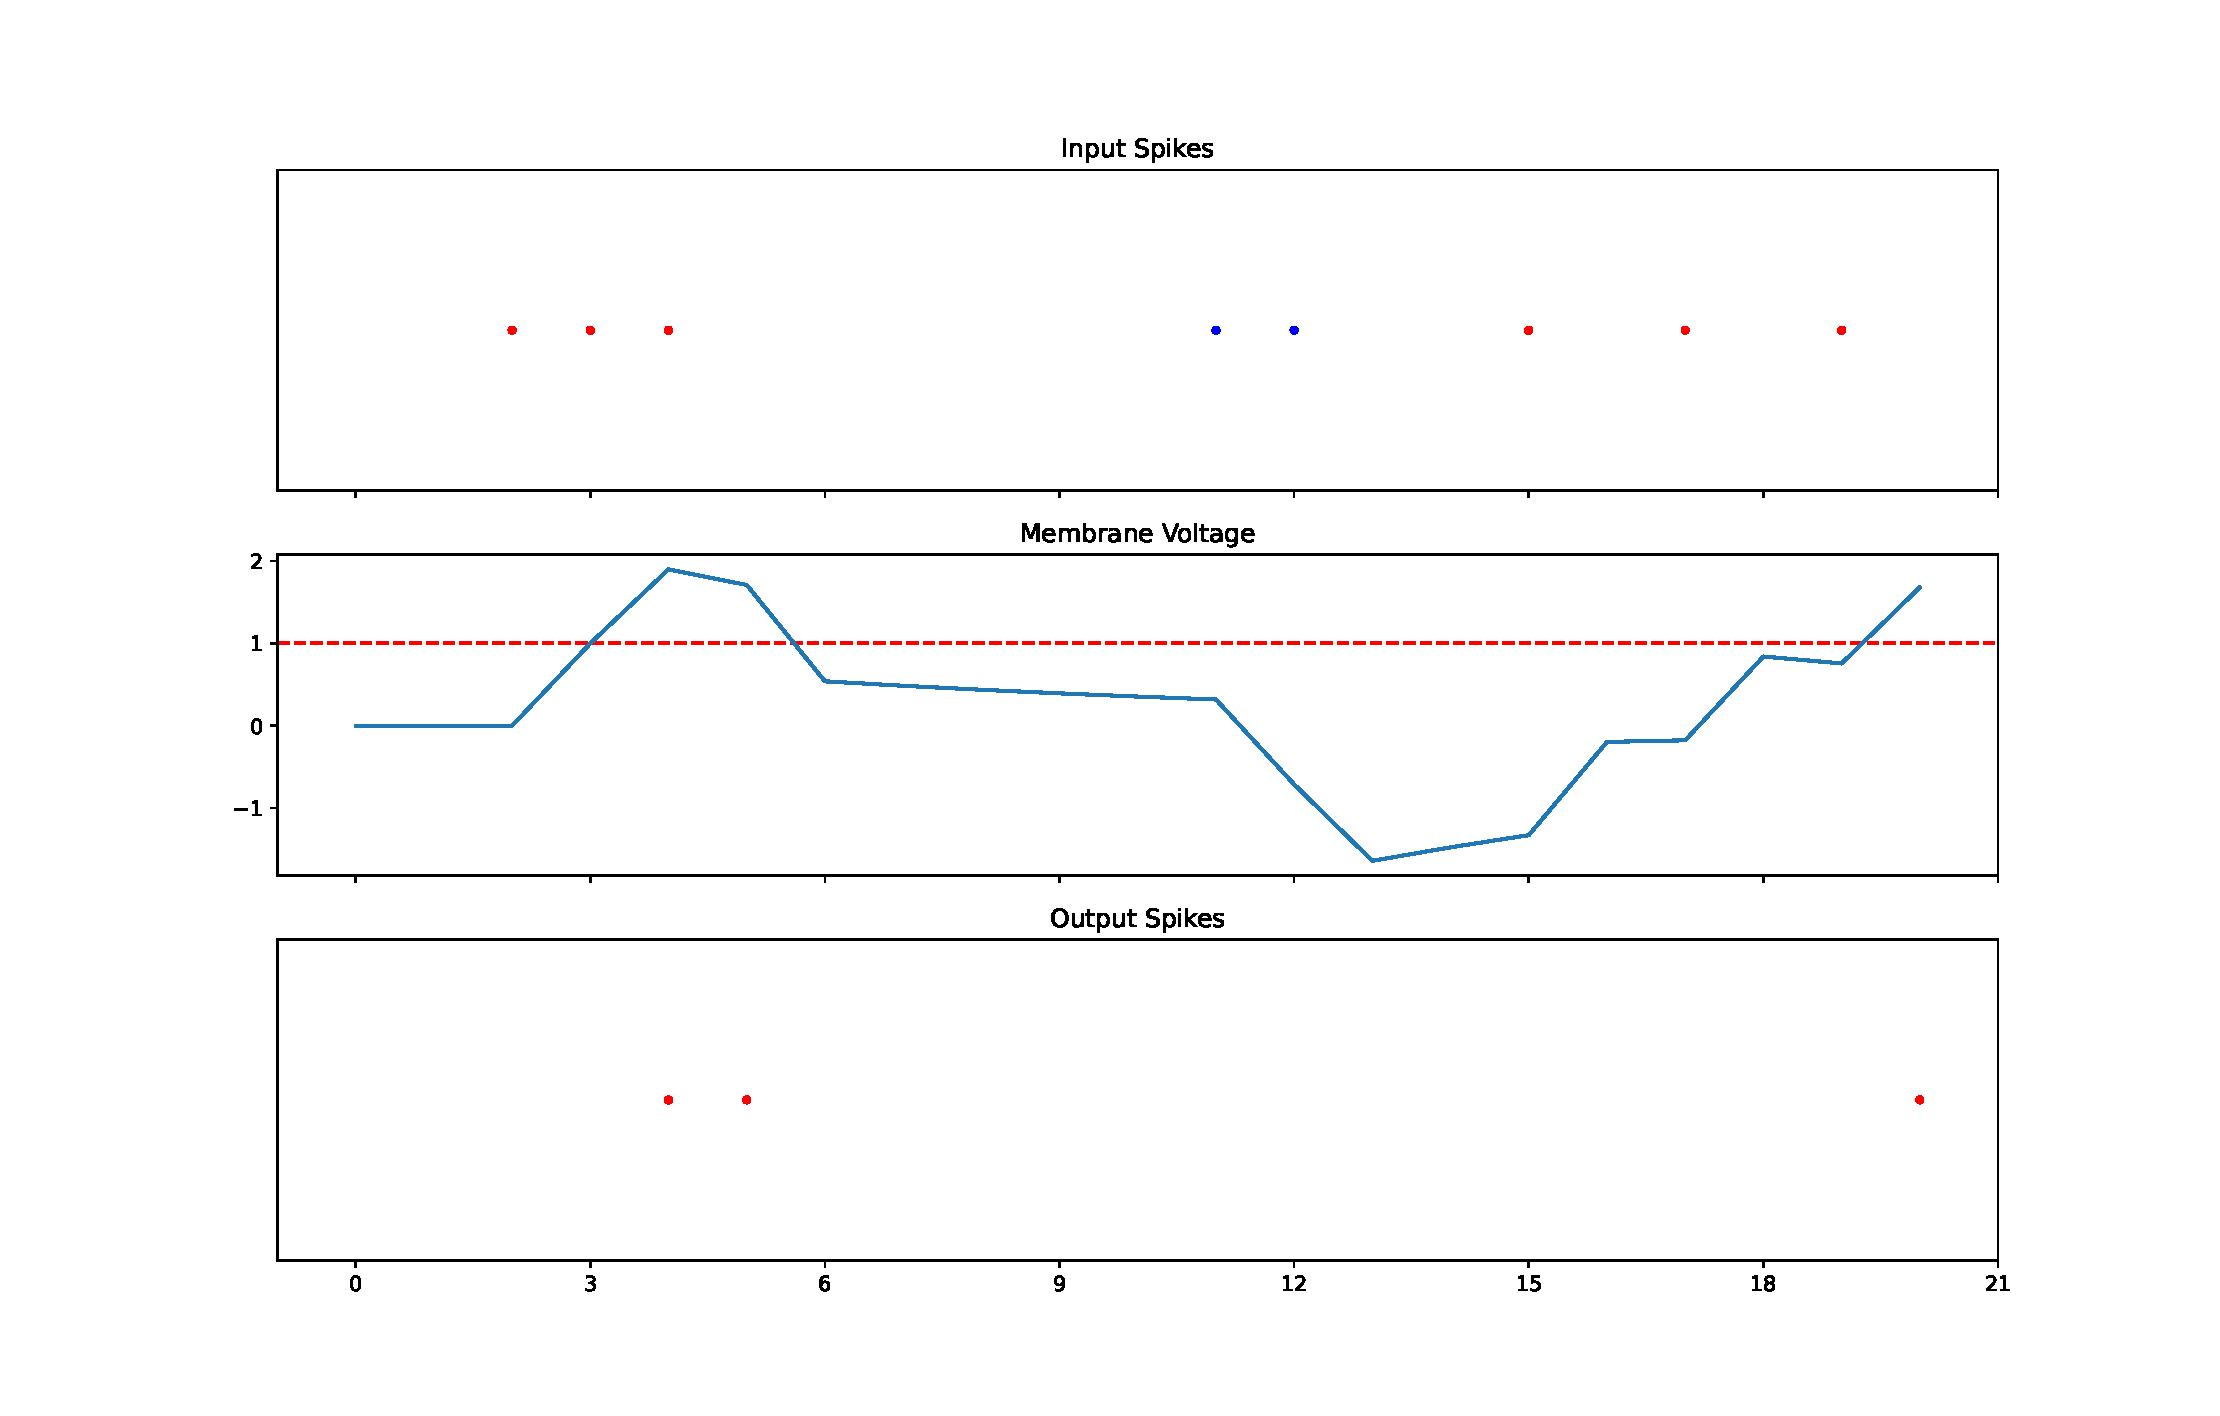
\includegraphics[width=\textwidth]{negative_spike_example}
    \caption[Negative spike inputs to a LIF neuron]{A neuron that receives negative spikes as input. Positive input spikes are shown in red, negative in blue. The membrane voltage increases with positive input spikes and crosses the threshold voltage to output spikes as well. When the negative spikes arrive as input, the membrane voltage decreases.}
    \label{fig:negative_spike_example}
\end{figure}

The inputs to the rate encoder can also be scaled up before being turned into spikes. This is referred to as the gain, which we treat as a hyperparameter. For example, given gain $g$ and input $x$, our new input becomes $g*x$. Values above 1 are clipped to 1.

Larger gain values seemed to create a smoother decrease in loss and better training performance. Intuitively this makes sense because this creates more spikes in the input layer and gives downstream neurons more opportunities to fire. However, larger gain values also led to higher validation loss and resulted in models that could not track the target during inference. We limit the amount of gain to 2, meaning that photoreceptors with values 0.5 and above spiked at every timestep.

% loss graph of tuning gain?

%********************************************************************%

\subsubsection{Latency Encoding}

Latency encoding, on the other hand, focuses on the timing of spikes rather than the spikign frequency. Each neuron is allowed to fire once in the simulated time interval; neurons with a higher probability of firing emit their spike earlier than neurons with lower probabilities of spiking. This encoding method results in sparser inputs to the SNN when compared to rate encoding and as a result also makes it difficult for the model to converge.

Figure~\ref{fig:onv_encode_latency} contains spikes that result from latency encoding the onv from Figure~\ref{fig:onv_prev}. In the figure we see that very excited neurons fire at the first timestep and partially excited neurons fire sometime afterwards. The spikes at the last timestep represent inputs of 0.

\begin{figure}
    \centering
    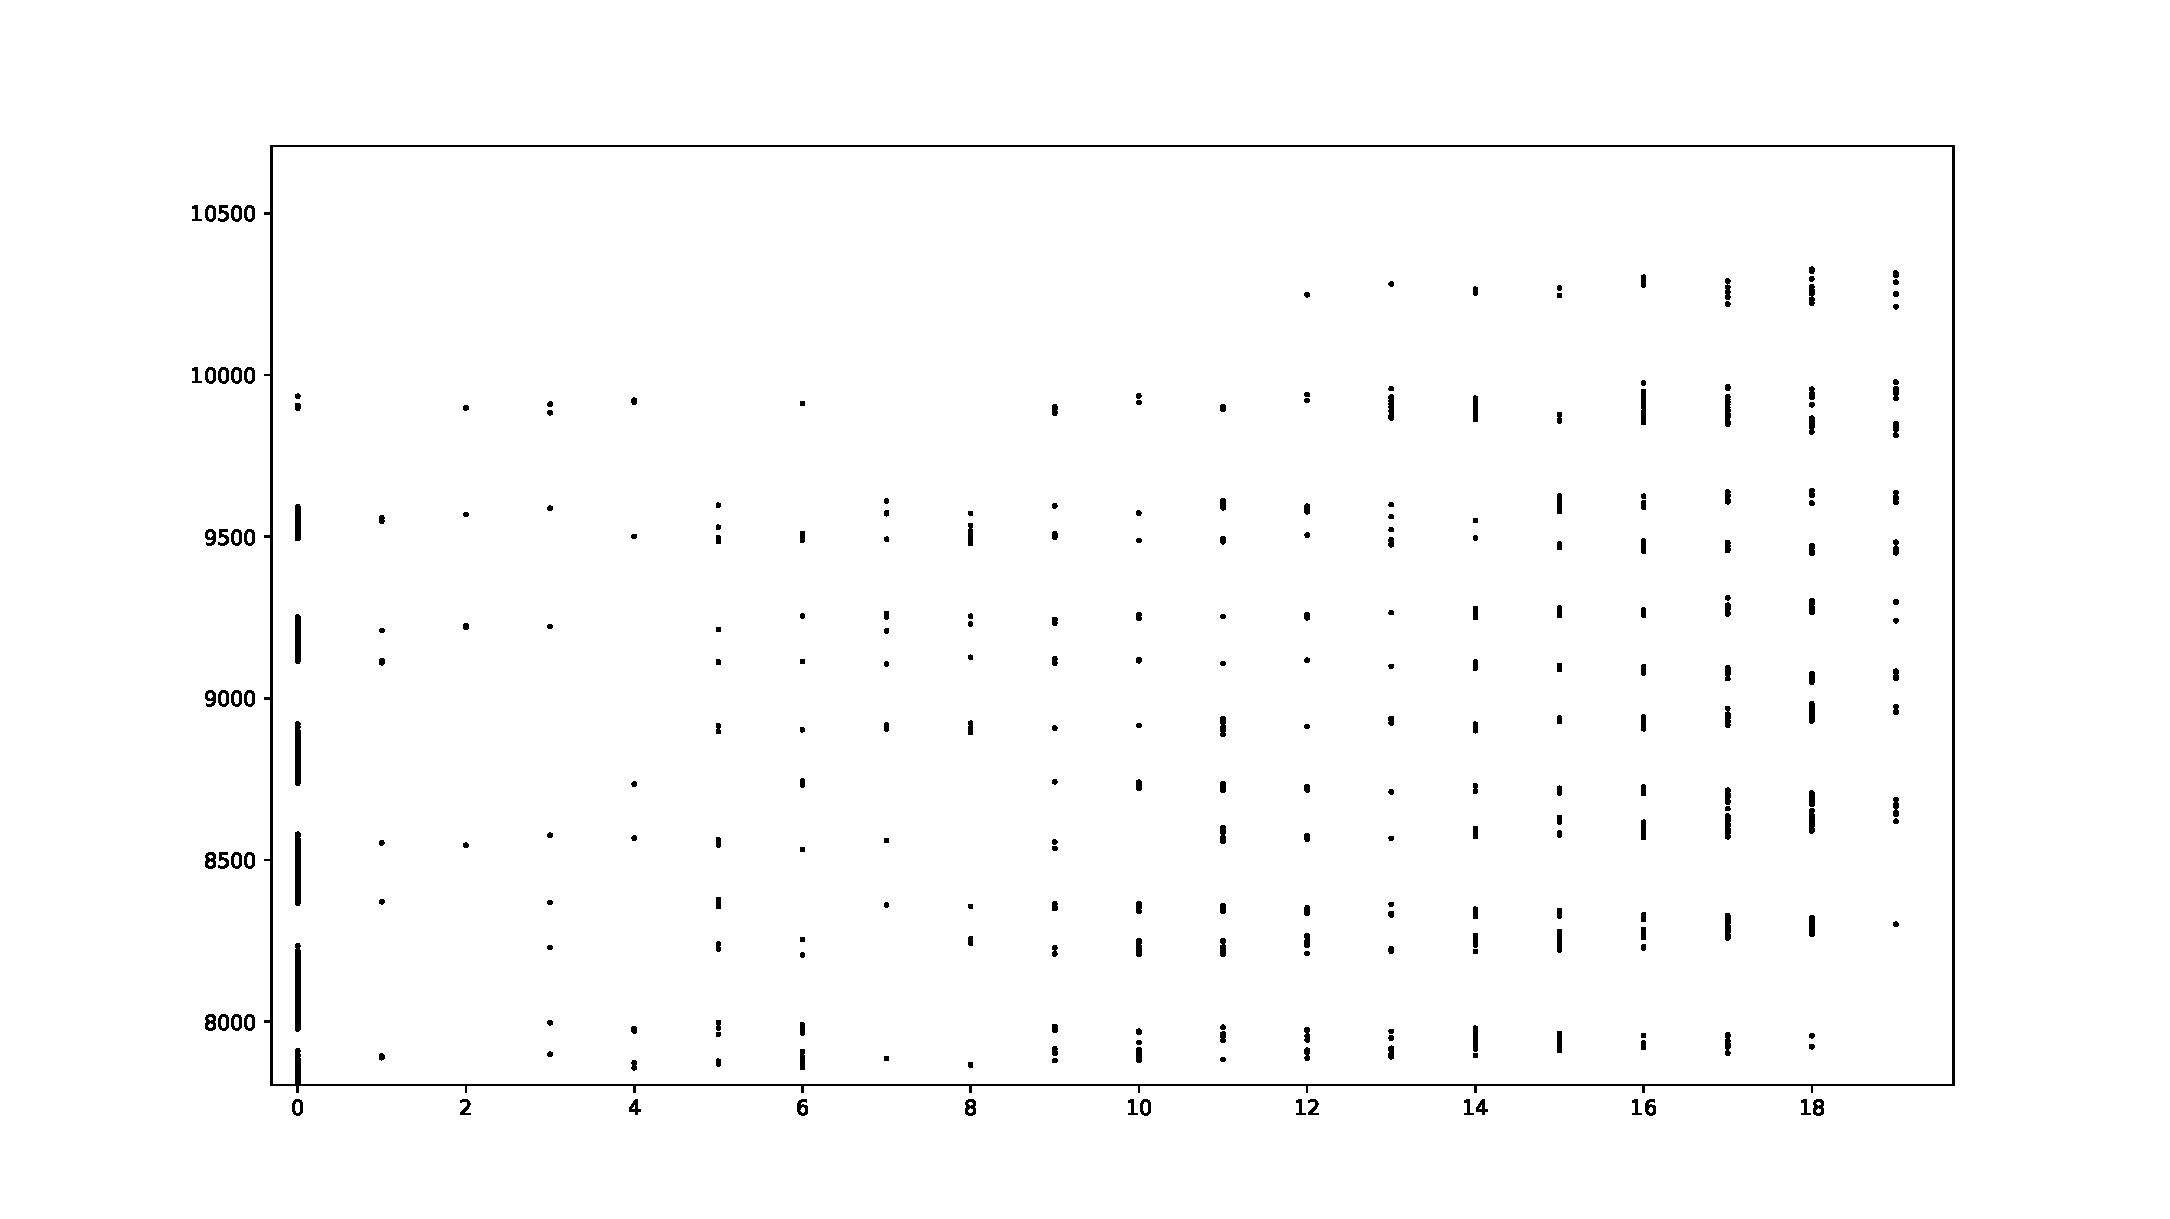
\includegraphics[width=\textwidth]{onv_latency_prev}
    \caption[Latency encoded ONV]{Latency encoding of a subset of photoreceptors from the ONV in Figure~\ref{fig:onv_prev}. The values are normalized to fit within a 20 timestep range. Spikes to the left have the most excited neurons while the values to the right have less excited neurons.}
    \label{fig:onv_encode_latency}
\end{figure}

%%%%%%%%%%%%%%%%%%%%%%%%%%%%%%%%%%%%%%%%%%%%%%%%%%%%%%%%%%%%%%%%%%%%%%

\chapter{The Model}

In this chapter we discuss how we base our SNN architecture on that of a LiNet.

\section{Architecture}

We base our SNN architecture on that of the LiNet developed by \citet{Masaki}. The LiNet was designed for this task and vastly outperforms fully connected networks. More information about LiNets is provided in appendix \ref{appendix:linet}. To summarize the architecture, it has 5 locally connected layers with one fully connected layer at the end. Each layer has $1/5$ the number of neurons as the previous layer. 

To build our SNN, we start with a 4 layer LiNet and replace the ReLU activations with spiking neurons. We keep the fully connected output layer to transform the membrane voltages into our two angles. Our SNN model is summarized in Figure~\ref{fig:linet_arch} and a simple code example is shown in Listing~\ref{listing:snn_forward}.

\begin{figure}
    \centering
    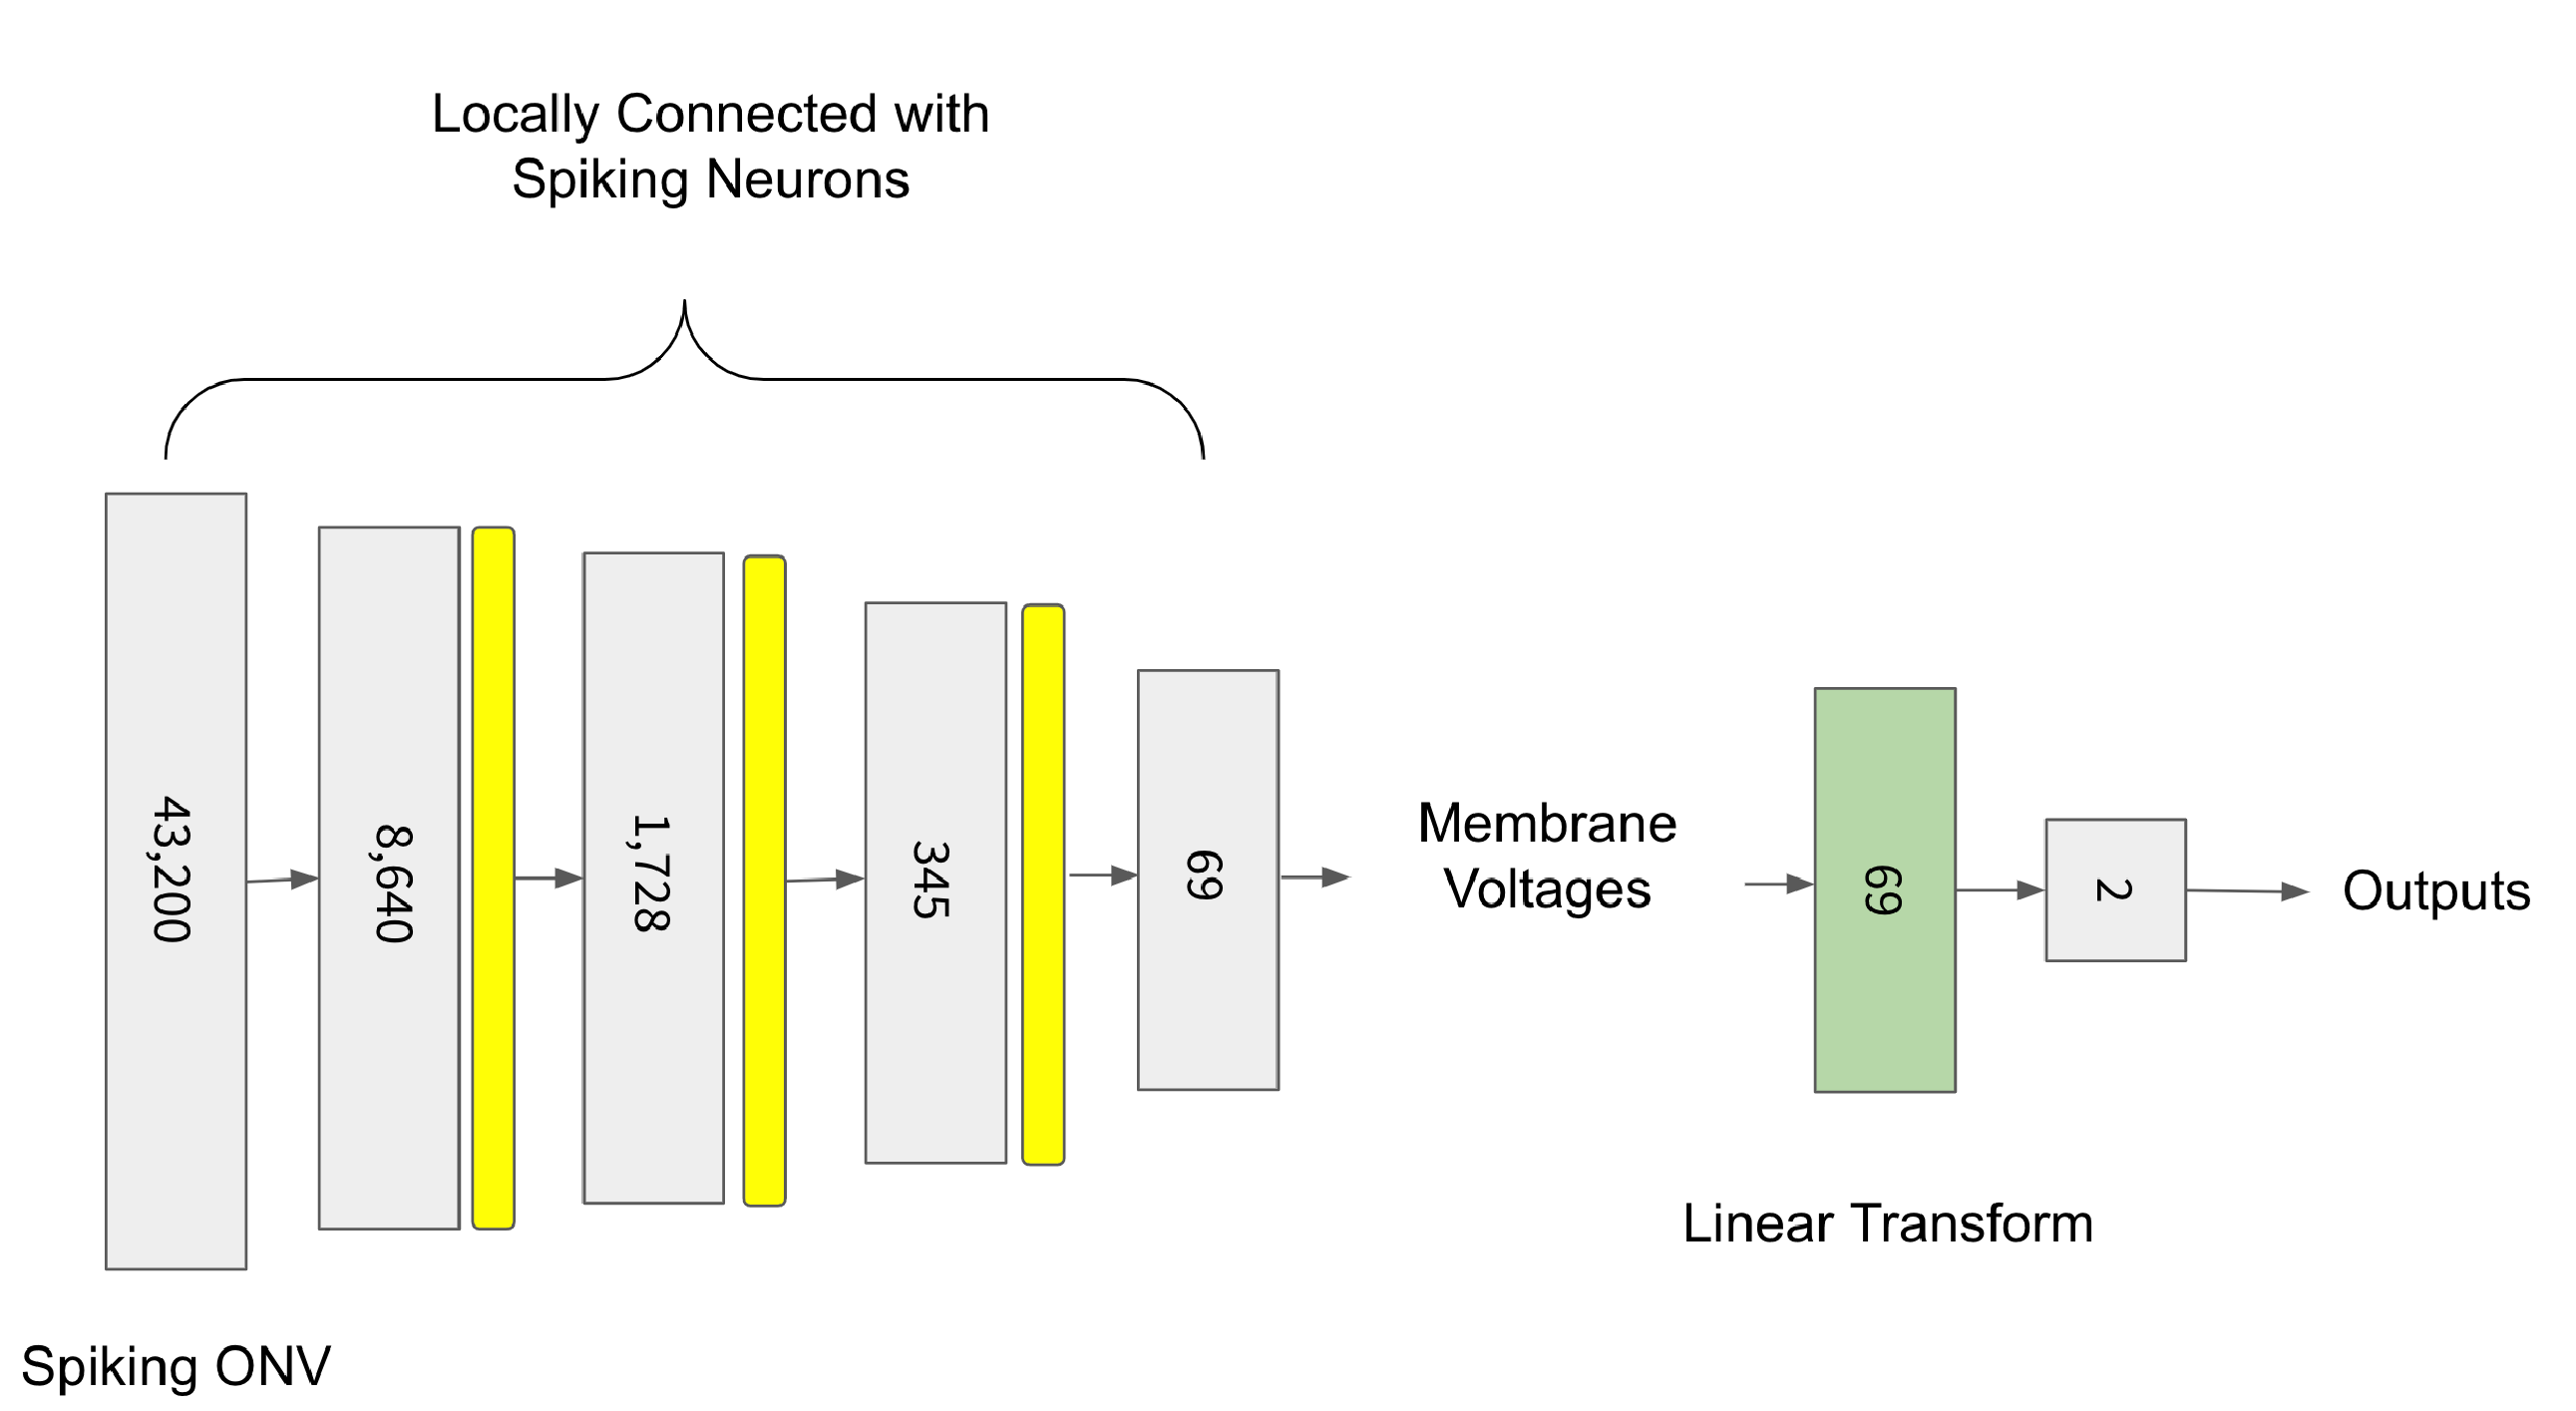
\includegraphics[width=\textwidth]{arch_spiking}
    \caption[SNN architecture]{Our spiking LiNet architecture.}
    \label{fig:linet_arch}
\end{figure}

\lstinputlisting[label={listing:ann_forward},language=Python, firstline=1, lastline=12, caption={Normal feedforward network.}]{figures/code1.py}

\lstinputlisting[label={listing:snn_forward},language=Python, firstline=15, lastline=35, caption={SNN feedforward network. Differences from listing \ref{listing:ann_forward} include the use of spiking neurons, time-varying input, and the use of a linear layer which transforms membrane voltages from the last layer. }]{figures/code1.py}

% Hybrid model
% \begin{figure}
%     \centering
%     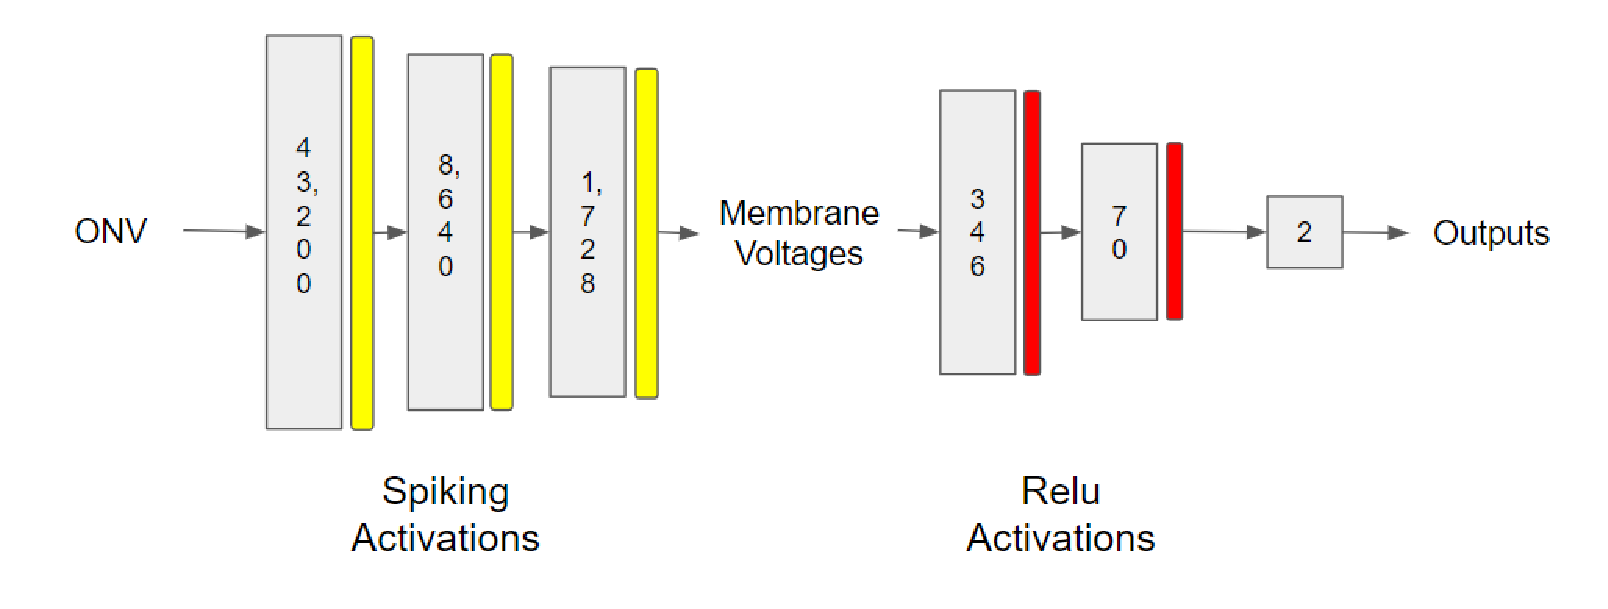
\includegraphics[width=\textwidth]{arch_hybrid}
%     \caption[Hybrid SNN architecture]{Our Hybrid Spiking LiNet architecture.}
%     \label{fig:hybrid_arch}
% \end{figure}

% We were also curious to see the effects of using ReLU activations with spiking activations. We call these models ``hybrid SNNs.'' The architecture has 5 locally connected layers where the first n layers have spiking inputs and the last few use ReLU. There is still one fully connected output layer. The spiking layers compute for a certain number of timesteps and then pass their membrane voltages to the artificial neuron half. This architecture is summarized in Figure~\ref{fig:hybrid_arch}, with a code example shown in Listing~\ref{listing:hybrid_forward}.

% code comparison between ANN, SNN, and Hybrid
% \noindent\begin{minipage}{.45\textwidth}
% \lstinputlisting[label={listing:ann_forward},language=Python, firstline=1, lastline=12, caption={Normal feedforward network.}]{figures/code1.py}
% \end{minipage}\hfill
% \begin{minipage}{.45\textwidth}
% \lstinputlisting[label={listing:snn_forward},language=Python, firstline=15, lastline=35, caption={SNN feedforward network. Differences from listing \ref{listing:ann_forward} include the use of spiking neurons, time-varying input, and the use of a linear layer which transforms membrane voltages from teh last layer. }]{figures/code1.py}
% \end{minipage}

% \lstinputlisting[label={listing:hybrid_forward}, language=Python, firstline=37, lastline=59, caption=A hybrid SNN that hands off the membrane voltages from its final spiking layer to linear layers that use the ReLU activation function.]{figures/code1.py}

% We noticed that adding spiking layers increases noise in the output. With this model, one can make a decision to use a certain number of layers to tradeoff between power usage/latency and accuracy. It also makes computation easier; one can imagine a neuromorphic chip finishing it computation and handing off the result to traditional GPU cores to finish inference. This method only uses the more expensive GPU cores for inference on a lower dimensional vector.

%********************************************************************%

\section{Training}

Here we go over the various decisions made while training our SNNs.

We train our models for around 100 epochs, which is around when the loss values start to plateau. We plot the training and validation losses for both a 5 layer LiNet and our 4 layer SNN. Figure~\ref{fig:loss_normal} contains the plots for each model trained with the normal ONV and Figure~\ref{fig:loss_delta} contains the plots for each model trained with the delta ONV. In both plots we can see that the LiNet achieves loss values one order of magnitude smaller than the spiking models. However, the spiking models still converge to low loss values. The LiNet validation loss is much higher when using the delta ONV, which may indicate that it will have trouble generalizing to our test scenarios.
% We can see the effect of including a ReLU activated layer in the hybrid model as it has slightly lower training and validation loss than the SNN achieves. 

With the delta ONV, the LiNet validation loss is much higher than when using the normal ONV. 
% Again the Hybrid SNN architecture achieves slightly lower loss values than the pure SNN architecture's loss values.

\begin{figure}
    \centering
    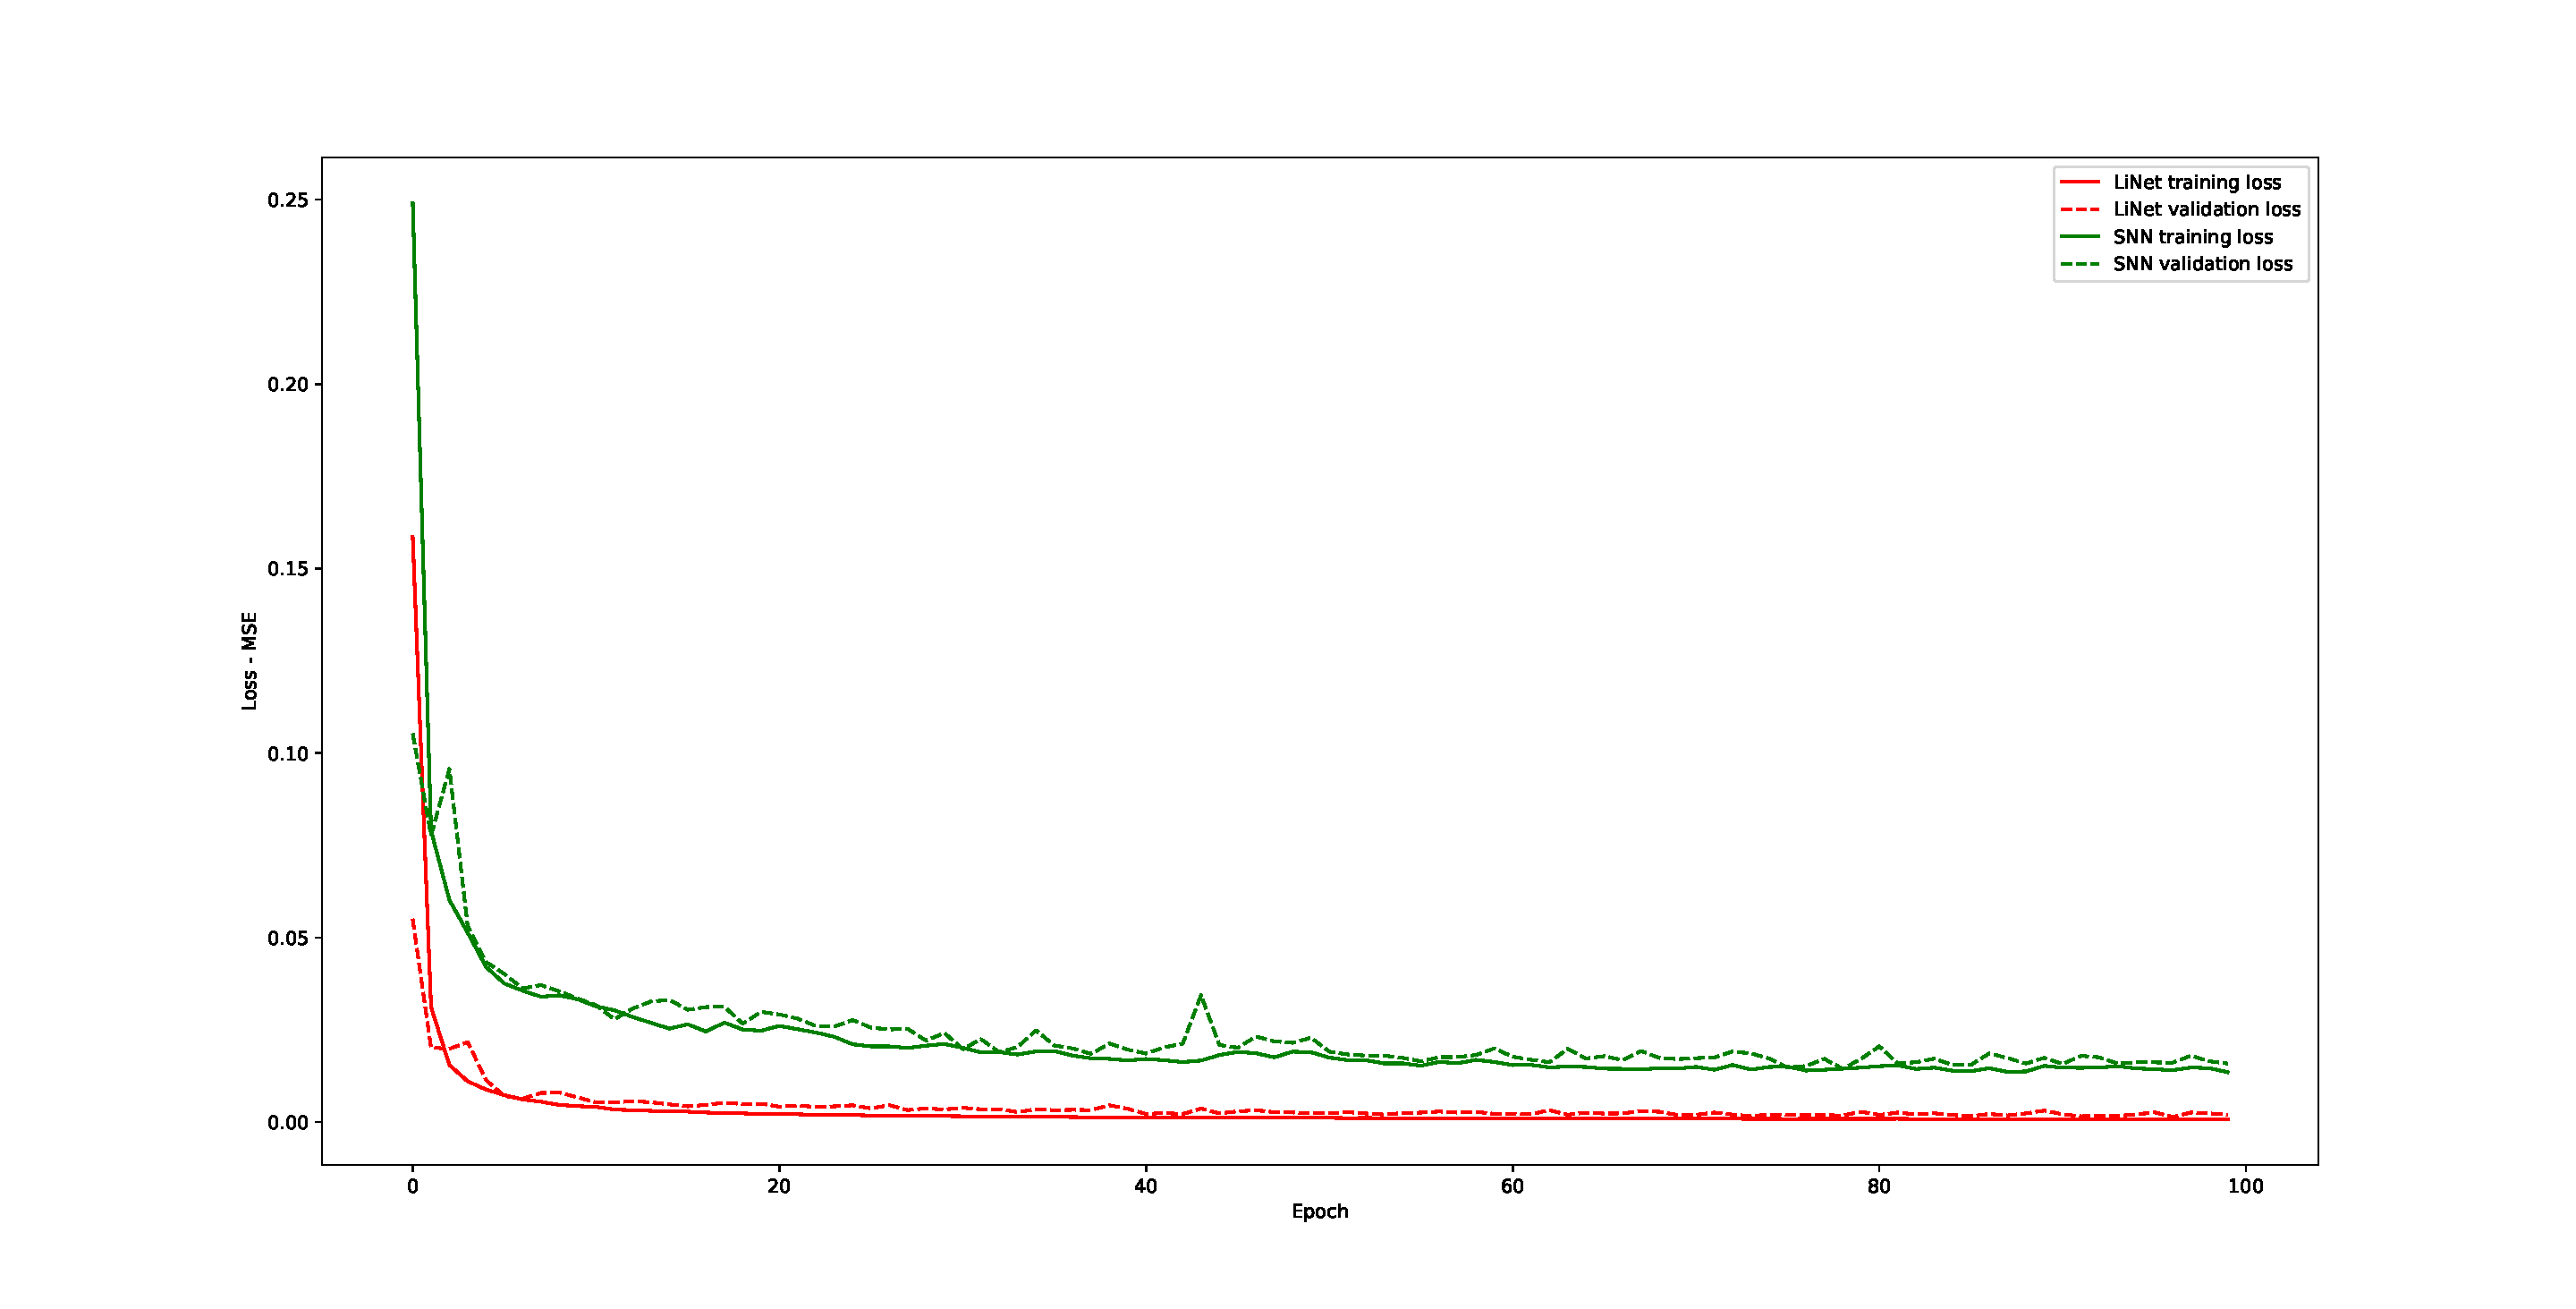
\includegraphics[width=\textwidth]{loss_normal}
    \caption[Training and validation loss using normal ONVs]{The LiNet converges very quickly and achieves a very low loss values. There is no indication of overfitting on either model as the validation loss continues to decrease with the training loss.}
    \label{fig:loss_normal}
\end{figure}

\begin{figure}
    \centering
    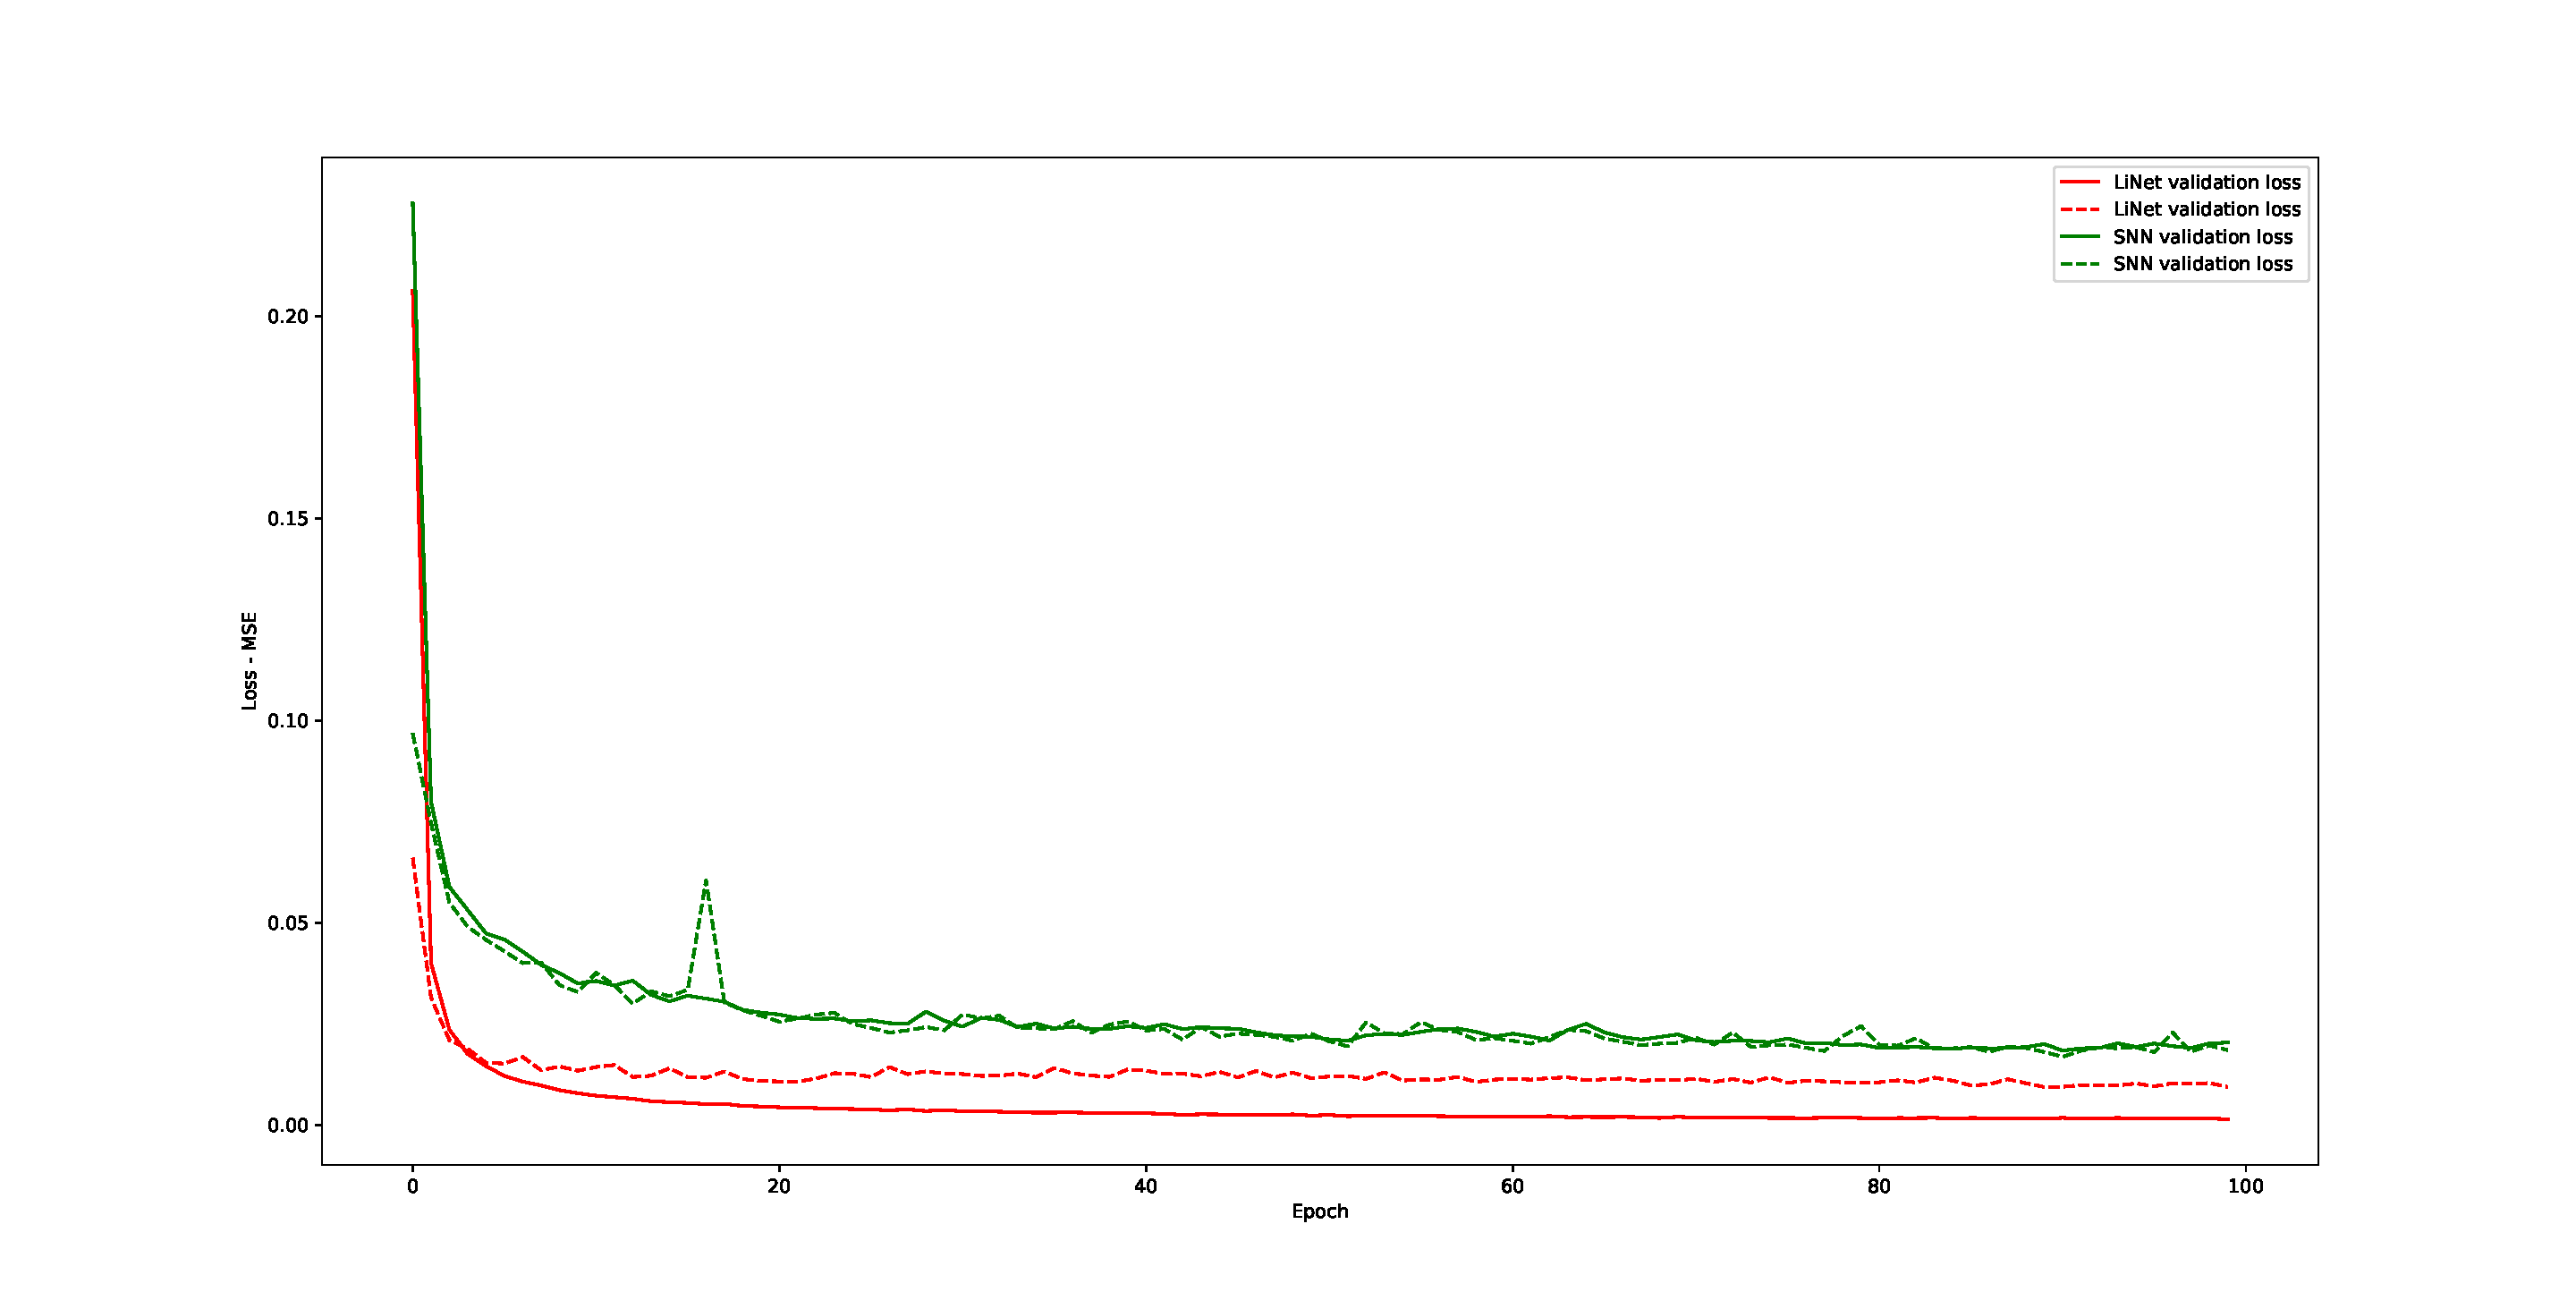
\includegraphics[width=\textwidth]{loss_delta}
    \caption[Training and validation loss using delta ONVs]{Again the LiNet converges quickly, but has high validation loss when using the delta ONV.}
    \label{fig:loss_delta}
\end{figure}

By default, all neuron thresholds are set to one and not trained. We treat the thresholds as trainable parameters during backpropagation and found that a random initialization converged better than initializing them to a value of one.

When a neuron outputs a spike, there are two options related to how to reset the membrane voltage. One is called ``zero'' because the voltage is simply set to zero. The other, called ``subtraction'', subtracts the threshold value instead. This allows the neuron to have a non-zero membrane voltage at the next timestep, where the reset happens. We empirically found that subtraction performs better than reset, which makes sense as there is less information lost after a spike.

\subsubsection{Number of Steps}

One hyperparameter is the length of the spiking input, otherwise referred to as the number of timesteps. This hyperparameter determines how many timesteps each neuron will have to accumulate voltage and emit spikes. More timesteps allow more downstream neurons to fire, which may help computation but will also require more energy to run. Conversely, models using a lower number of timesteps may train quickly but have difficulty converging to a low enough loss value. The typical number of timesteps ranges from the hundreds to thousands. After doing a hyperparameter sweep we empirically found that 20 timesteps was enough for our model to converge. Higher numbers of steps were more difficult to train and did not seem to affect performance.

% this is odd, have graphs of loss for various timesteps?


\subsubsection{Surrogate Gradients}

On the backpropagation pass, we encounter the Heaviside step function in our spiking activation function. Its local derivative is 0 everywhere except for the time of the spike, where it is infinite. This is the main barrier to deep learning with spiking neural networks as our gradient will either become 0 or infinity after reaching this function on the backward pass. snnTorch handles this by passing through the gradient when there is a spike and 0 when there isn’t. This enables some learning, but is not good enough for our task. We experimented with surrogate gradients, which are functions that approximate the Heaviside step function but are differentiable everywhere \citep{surrogate_grad}. The spiking activation is still used in the forward pass, but the surrogate gradient is used on the backward one.

% math of backprop with step func?

The approximation of choice is the fast sigmoid function, named as it is faster to compute than the normal sigmoid function. The function and its derivative are plotted in Figure~\ref{fig:surrogate_grad}. We find that the model fails to converge without the use of a surrogate gradient.

% figure of sigmoid and its derivative
\begin{figure}
    \centering
    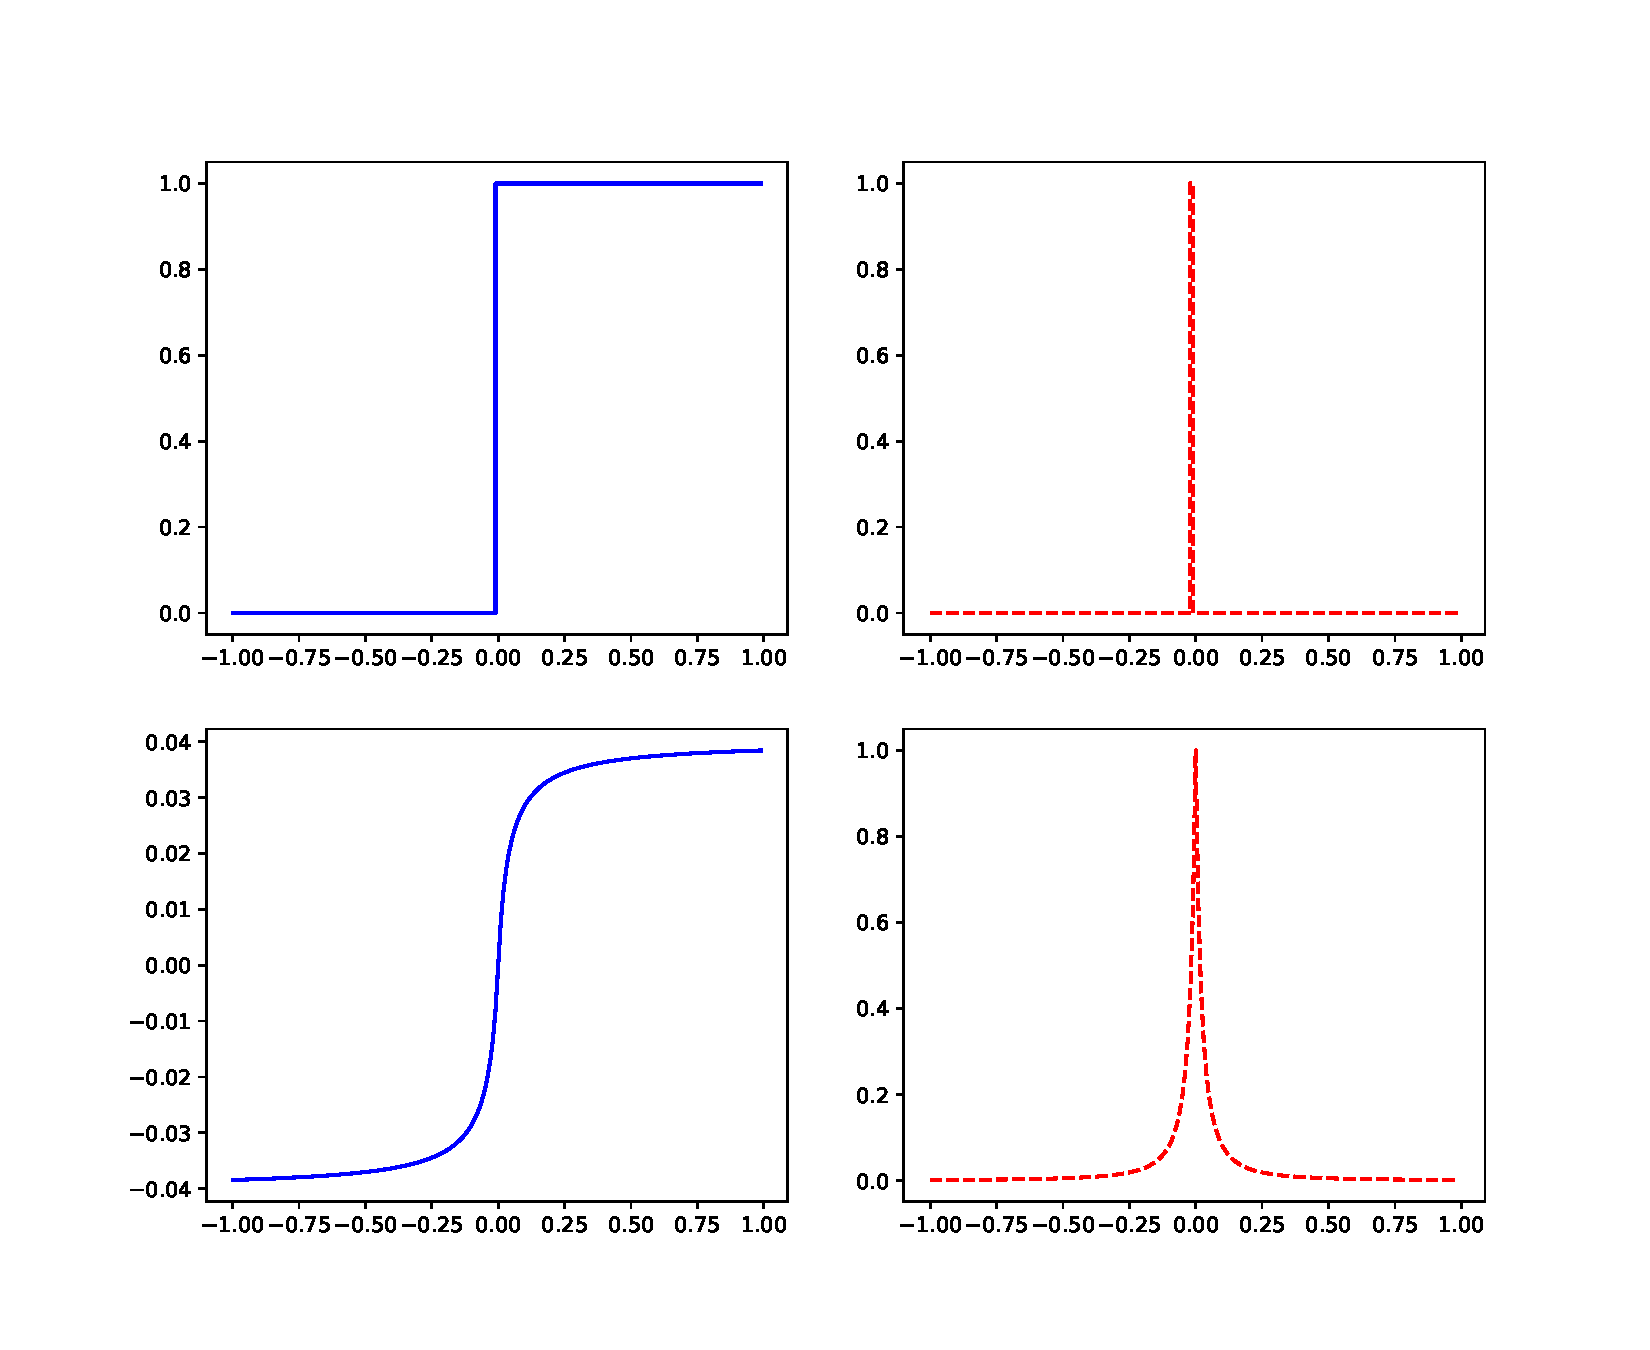
\includegraphics[width=\textwidth]{surrogate_grad}
    \caption[Derivatives of the Heaviside step and fast sigmoid functions]{We compare the derivative of the Heaviside step function and that of the fast-sigmoid function.}
    \label{fig:surrogate_grad}
\end{figure}

\subsubsection{Loss Calculation}

The SNN computation graph can be unrolled exactly like a recurrent neural network (RNN), so backpropagation through time (BPTT) is used during training. One trick can be employed to encourage the SNN to reach correct outputs faster. The technique involves collecting the output from each timestep, calculating the loss with the expected value, then summing all of these losses together. This unfortunately required more memory than our GPU could handle, so we could not experiment with this method. Because our model required a relatively low amount of timesteps to run, we utilized BPTT and looked back through all 20 timesteps.

%********************************************************************%

\section{Convert ANN}

The ideas from this section are relevant only if one is training an SNN from scratch, which is the approach taken in this thesis. However, we did want to compare the performance of our trained SNN to that of a converted one.

Inspired by \citet{rathi2020enabling}, we tried an approach where we first scaled the weights and biases as an initialization step. We then trained this model on the data using the fast sigmoid surrogate gradient. This model unfortunately did not converge so we cannot report on differences between training and converting a SNN on our object tracking task.

%%%%%%%%%%%%%%%%%%%%%%%%%%%%%%%%%%%%%%%%%%%%%%%%%%%%%%%%%%%%%%%%%%%%%%

\chapter{Experiments and Results}

We test if our SNN foveation controller can produce 3 of the eye movements used in the thesis of \cite{Arjun}. We run our SNNs with both the normal ONV and the delta ONV, using the performance of a  LiNet as a baseline to compare to.

%********************************************************************%

\section{Fixation}

This test does not involve any movement of the target. We keep the target still and observe how well it is kept in the center of the retina. An unrealistic model would fixate perfectly on the ball and not move, whereas a more realistic model allows the target to drift around the center of the fovea. These small movements are similar to micro-saccades in real eyes where a movement in one direction is balanced with a consecutive movement in the opposite direction. Figure~\ref{fig:fixation} shows this type of movement across four timesteps.

% TODO: describe figure more

\begin{figure}
    \centering
    \begin{subfigure}[b]{0.20\textwidth}
        \centering
        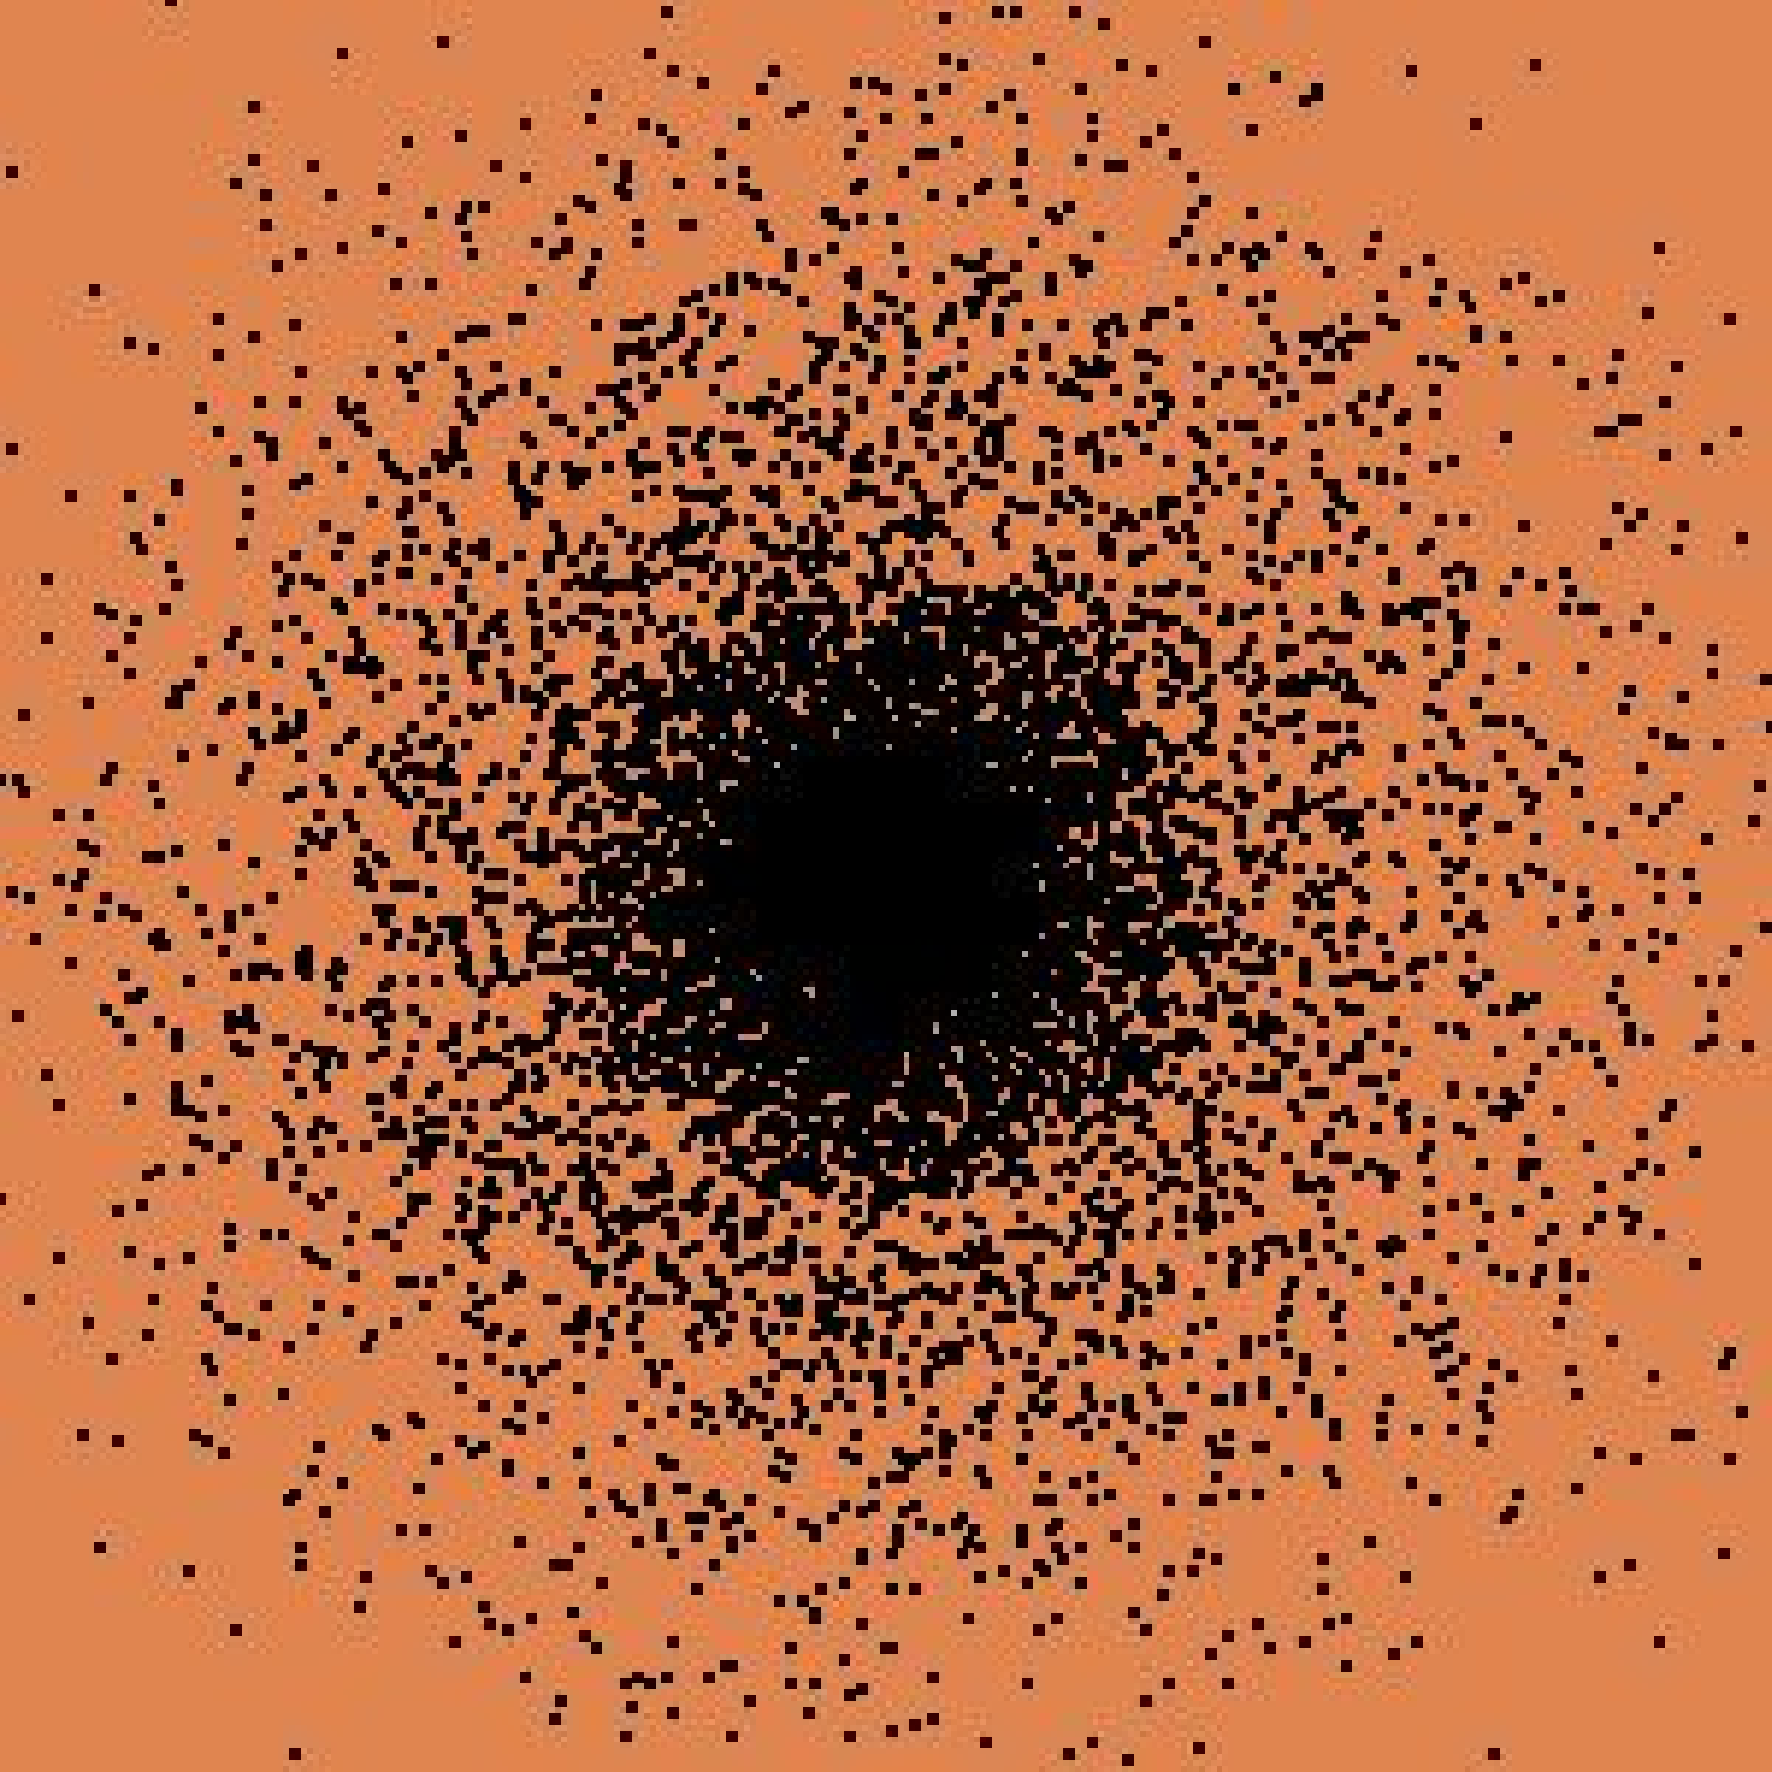
\includegraphics[width=\textwidth]{fixation2}
        \caption{}
    \end{subfigure}
    \hfill
    \centering
    \begin{subfigure}[b]{0.20\textwidth}
        \centering
        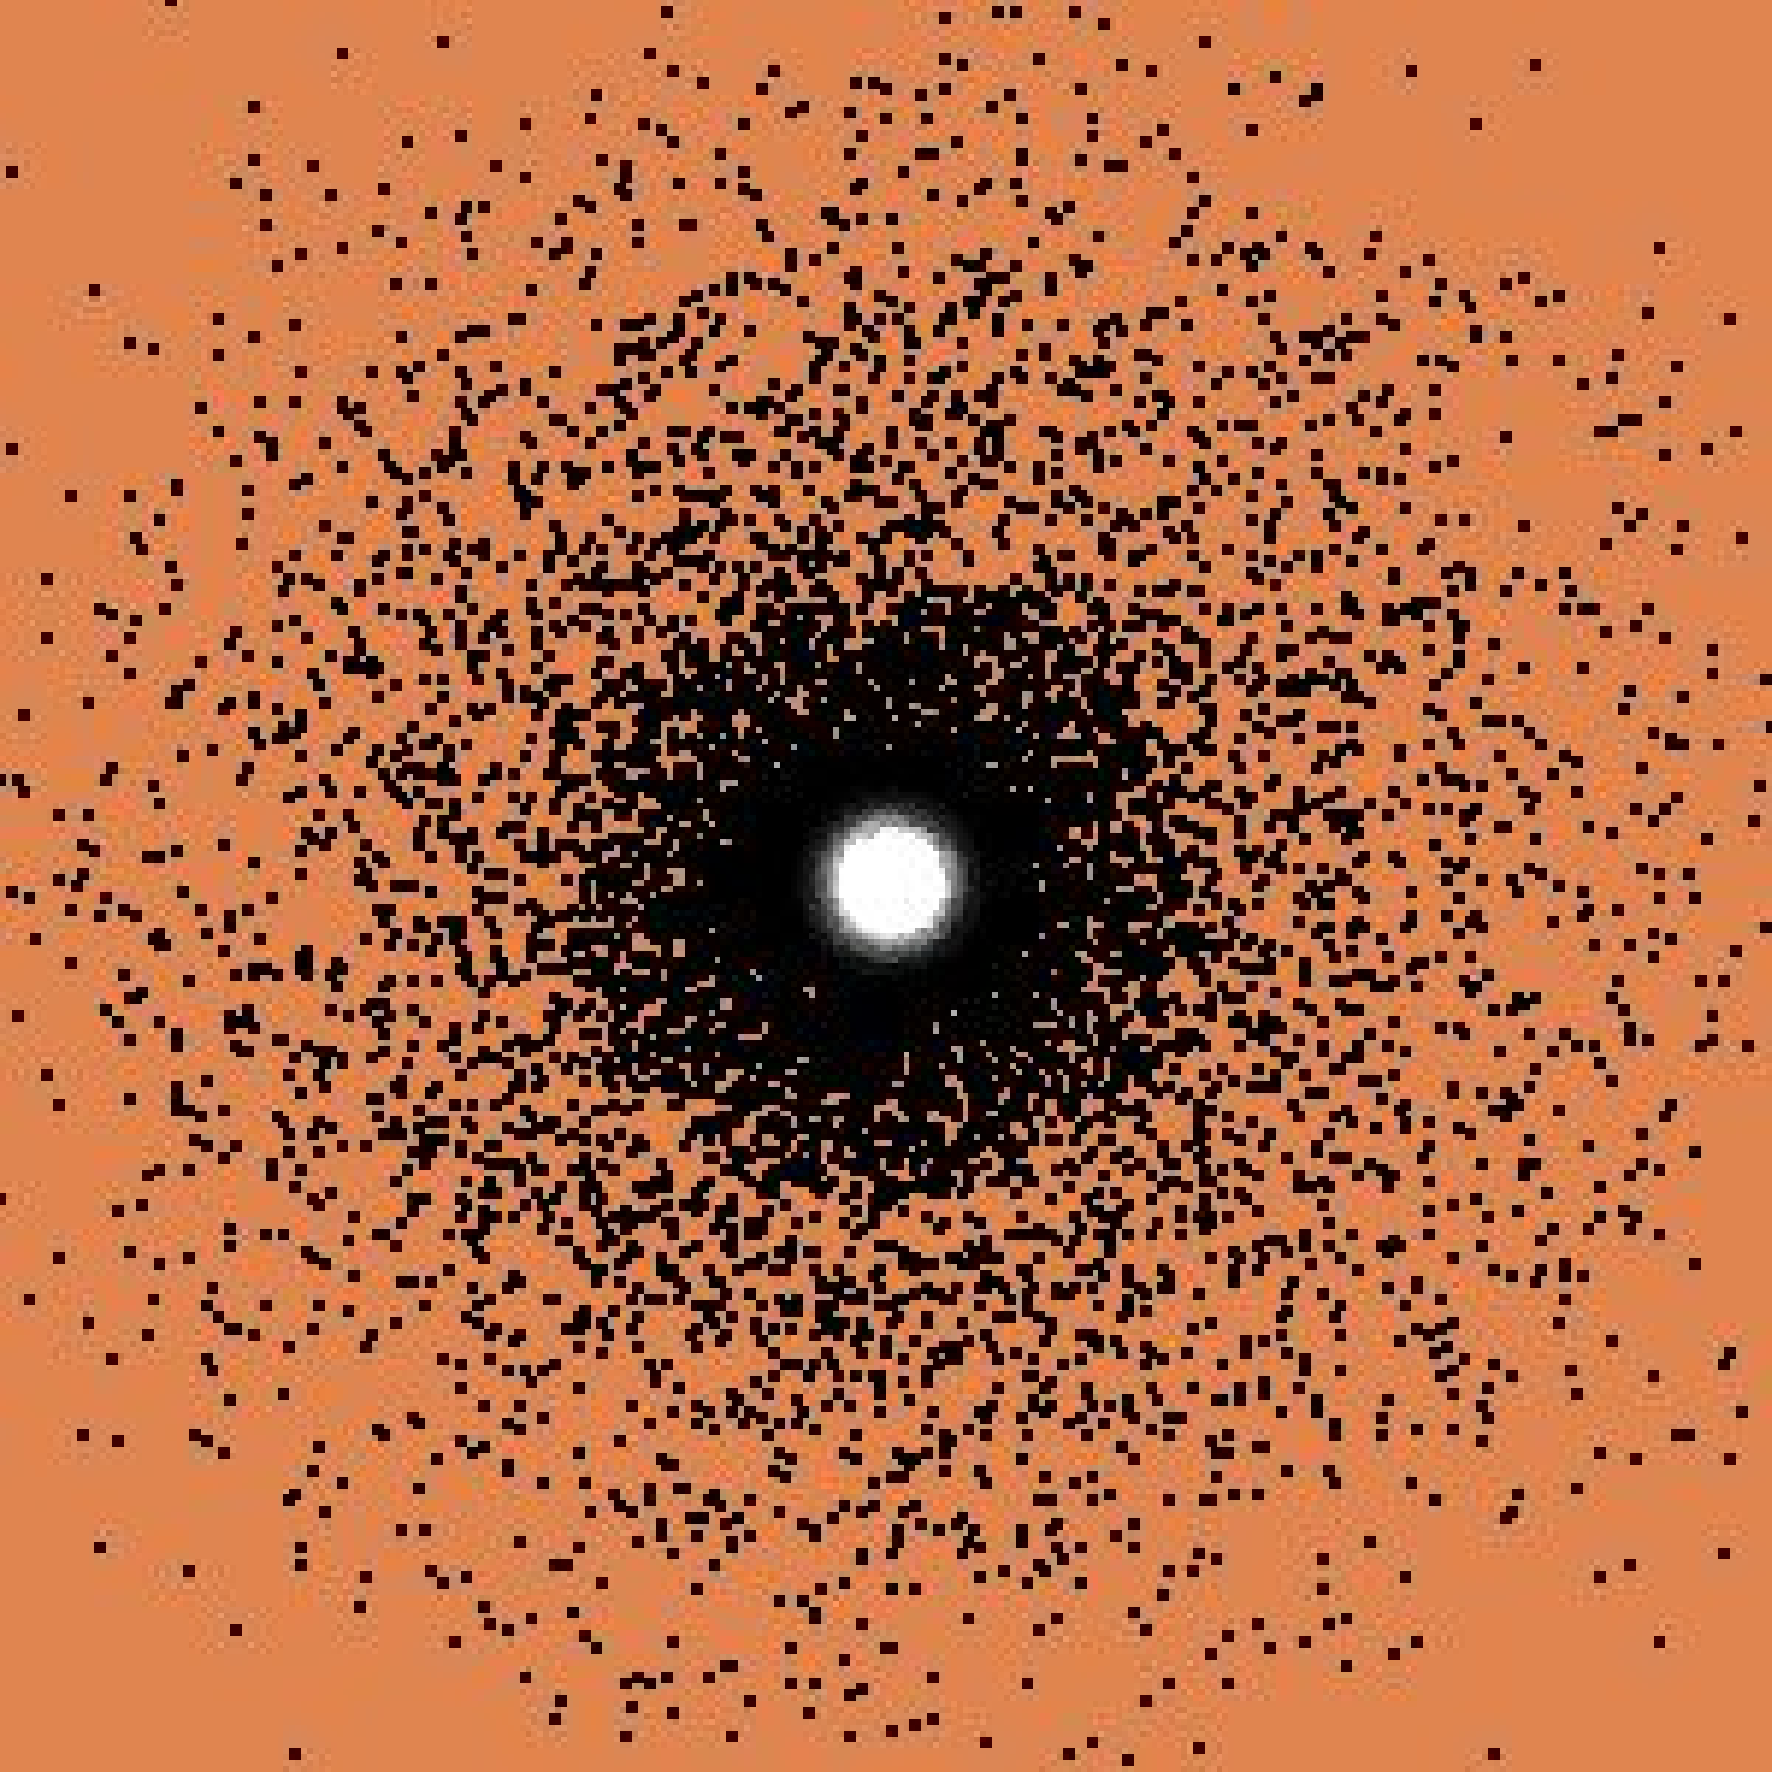
\includegraphics[width=\textwidth]{fixation3}
        \caption{}
    \end{subfigure}
    \hfill
    \centering
    \begin{subfigure}[b]{0.20\textwidth}
        \centering
        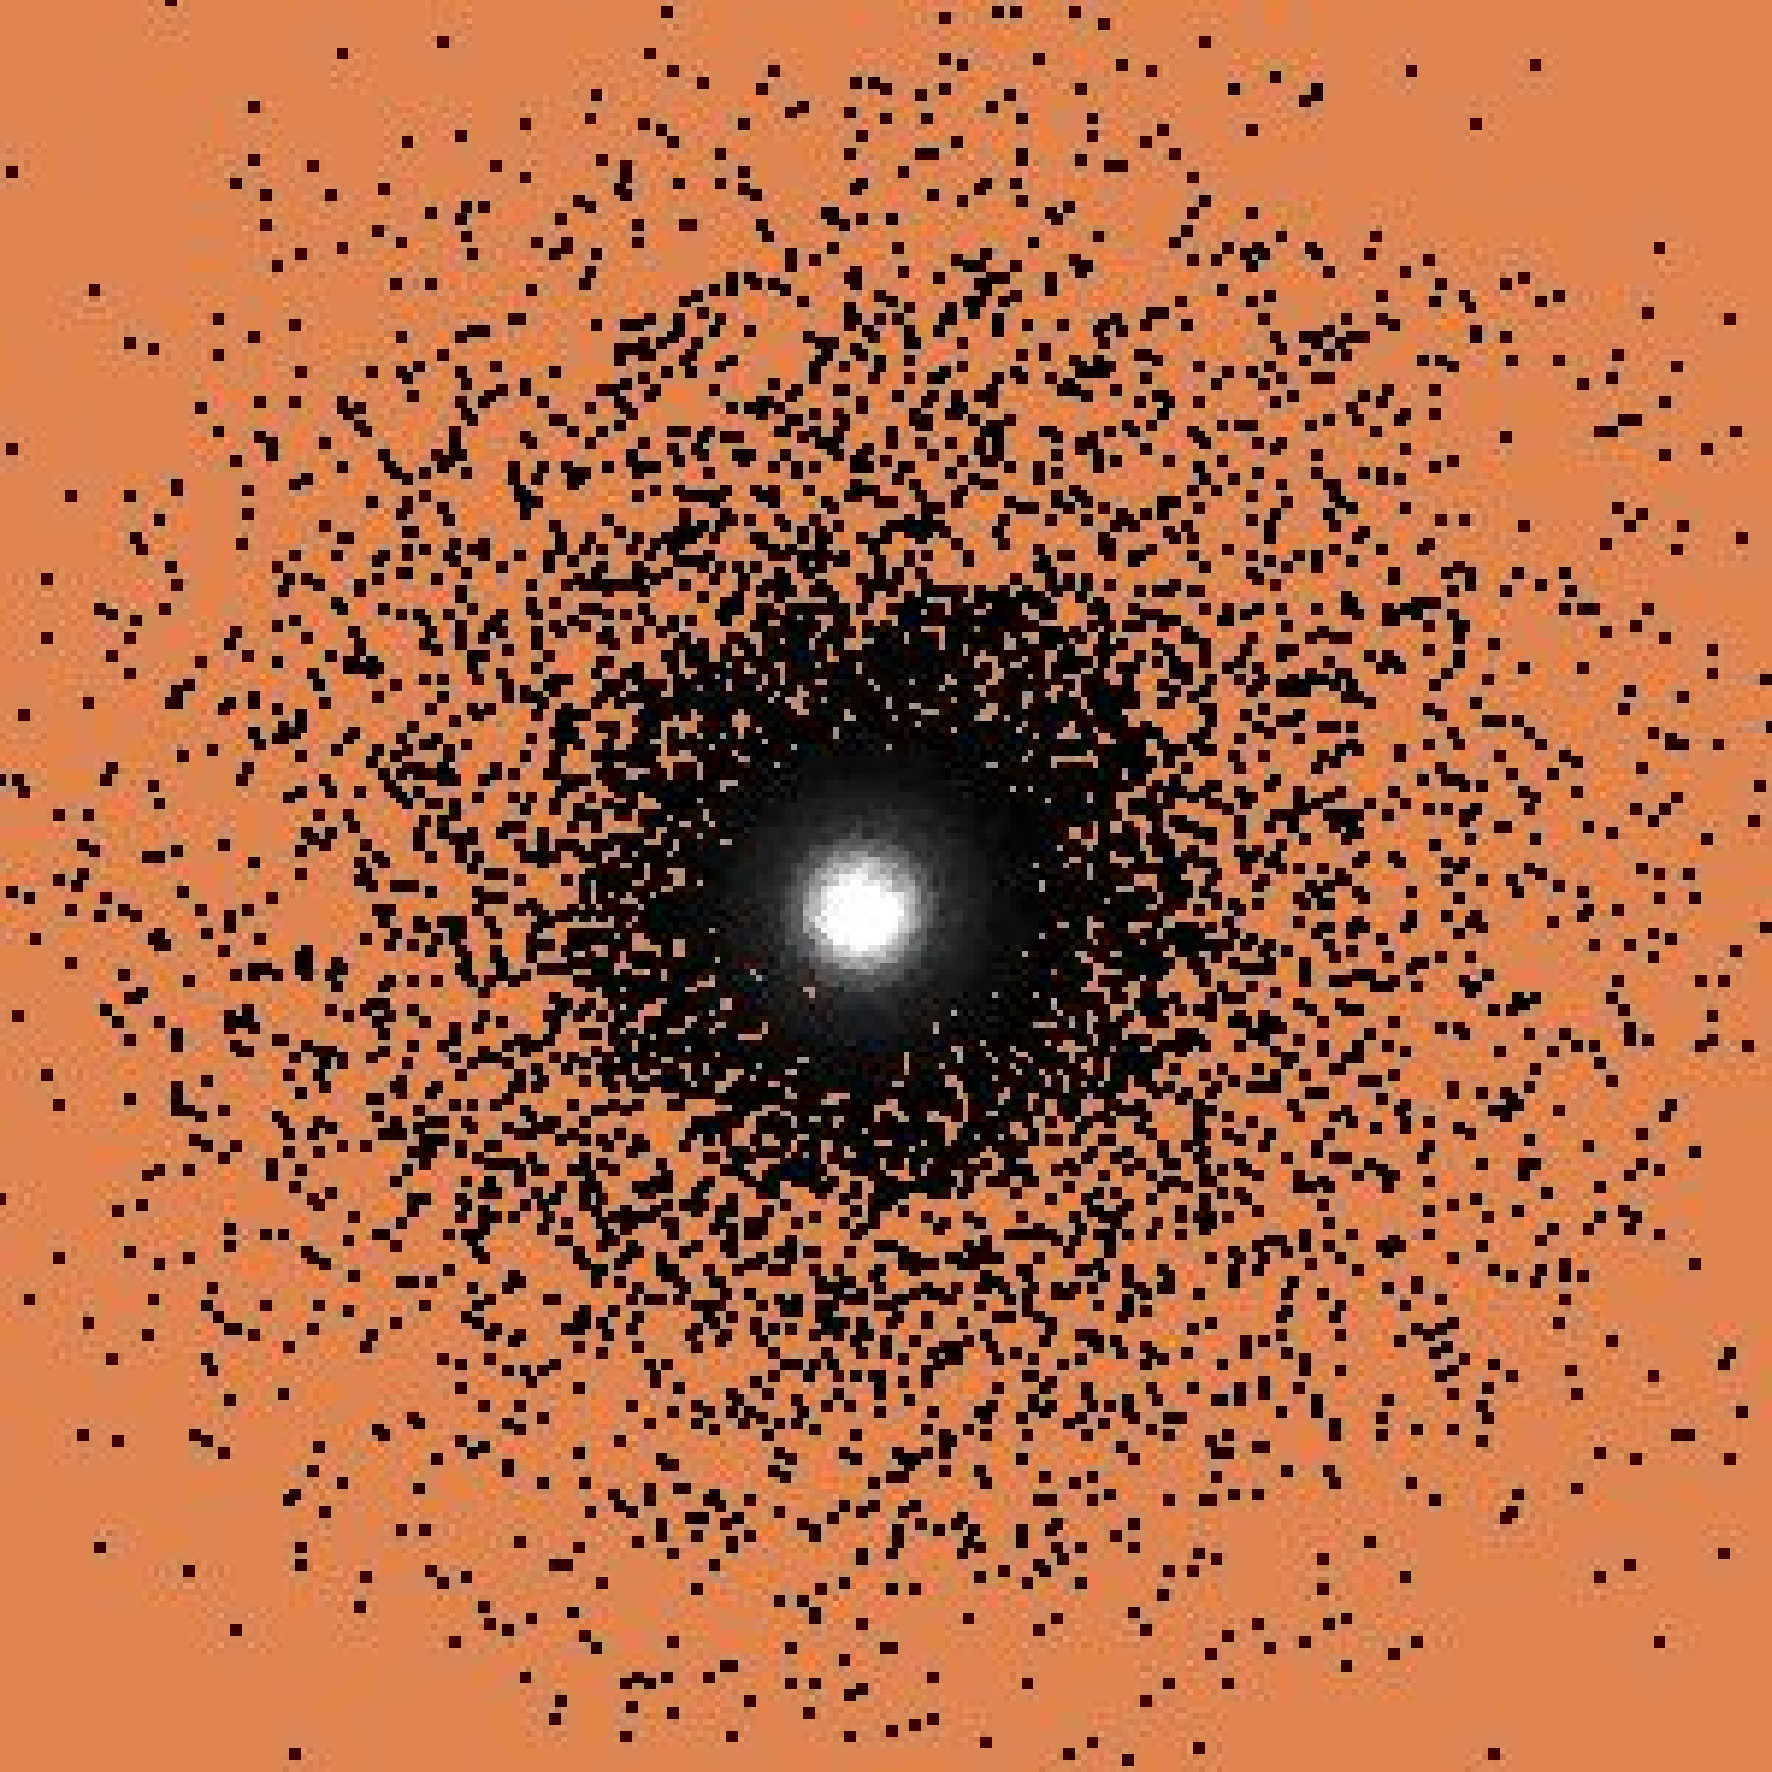
\includegraphics[width=\textwidth]{fixation4}
        \caption{}
    \end{subfigure}
    \hfill
    \centering
    \begin{subfigure}[b]{0.20\textwidth}
        \centering
        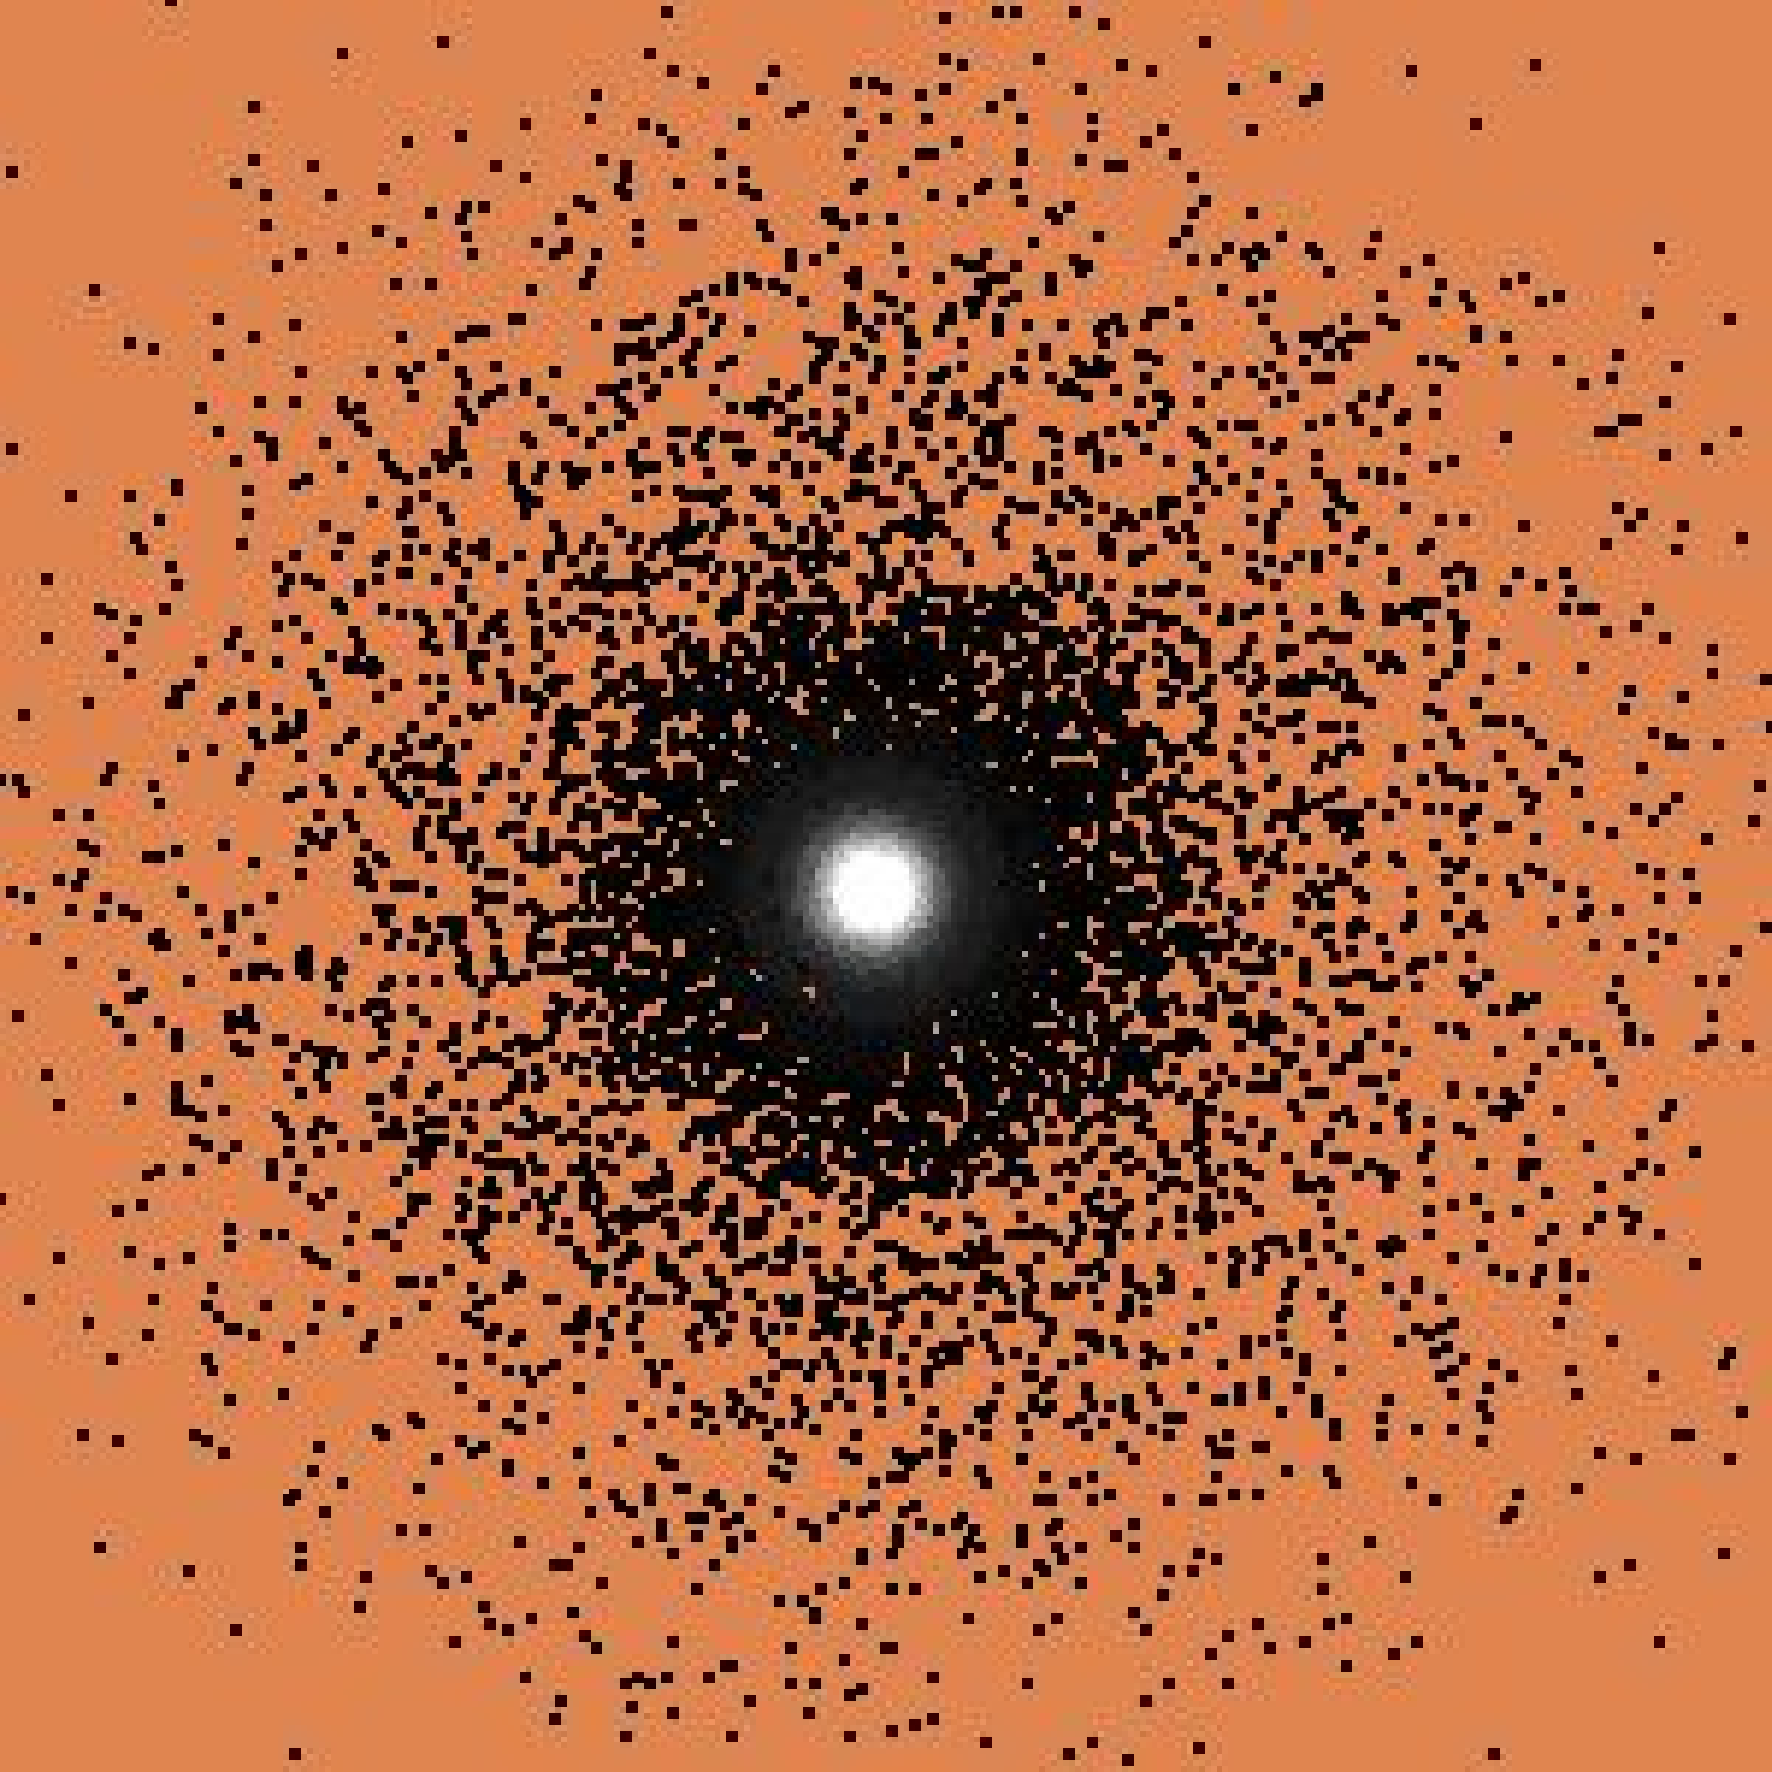
\includegraphics[width=\textwidth]{fixation5}
        \caption{}
    \end{subfigure}
    \caption[Fixation simulation with a SNN]{In (a), the ball has just entered the eye's field of view. In (b) the eye has fixated on the ball. In (c)-(d) we see micro-saccades in opposite directions.}
    \label{fig:fixation}
\end{figure}

%********************************************************************%

\section{Smooth Pursuit}

The smooth pursuit test moves the target slowly in both the horizontal and vertical directions. We observe if our SNN can successfully track this motion with $\theta$ and $\phi$ changing at the same time.

In Figure~\ref{fig:smooth} we compare the performance of a LiNet to that of our 4 layer SNN. The black lines represent the exact position that the eye's gaze should point at for each timestep. The orange lines track the performance of the LiNet architecture and the blue lines track the performance of our SNN. 

In Figure~\ref{fig:smooth_normal} we compare the performance of the models on the normal ONV. The LiNet performs much better here, and the ball leaves the center of the eye when using the SNN. In Figure~\ref{fig:smooth_delta} we see that the SNN performs better when a delta ONV but note that the motions are noisier than those of the LiNet. 
% Finally, in Figure~\ref{fig:smooth_hybrid} we see that using our Hybrid SNN with just ReLU activated layer results in smooth performance.

\begin{figure}
    \centering

    \begin{subfigure}[b]{0.8\textwidth}
        \centering
        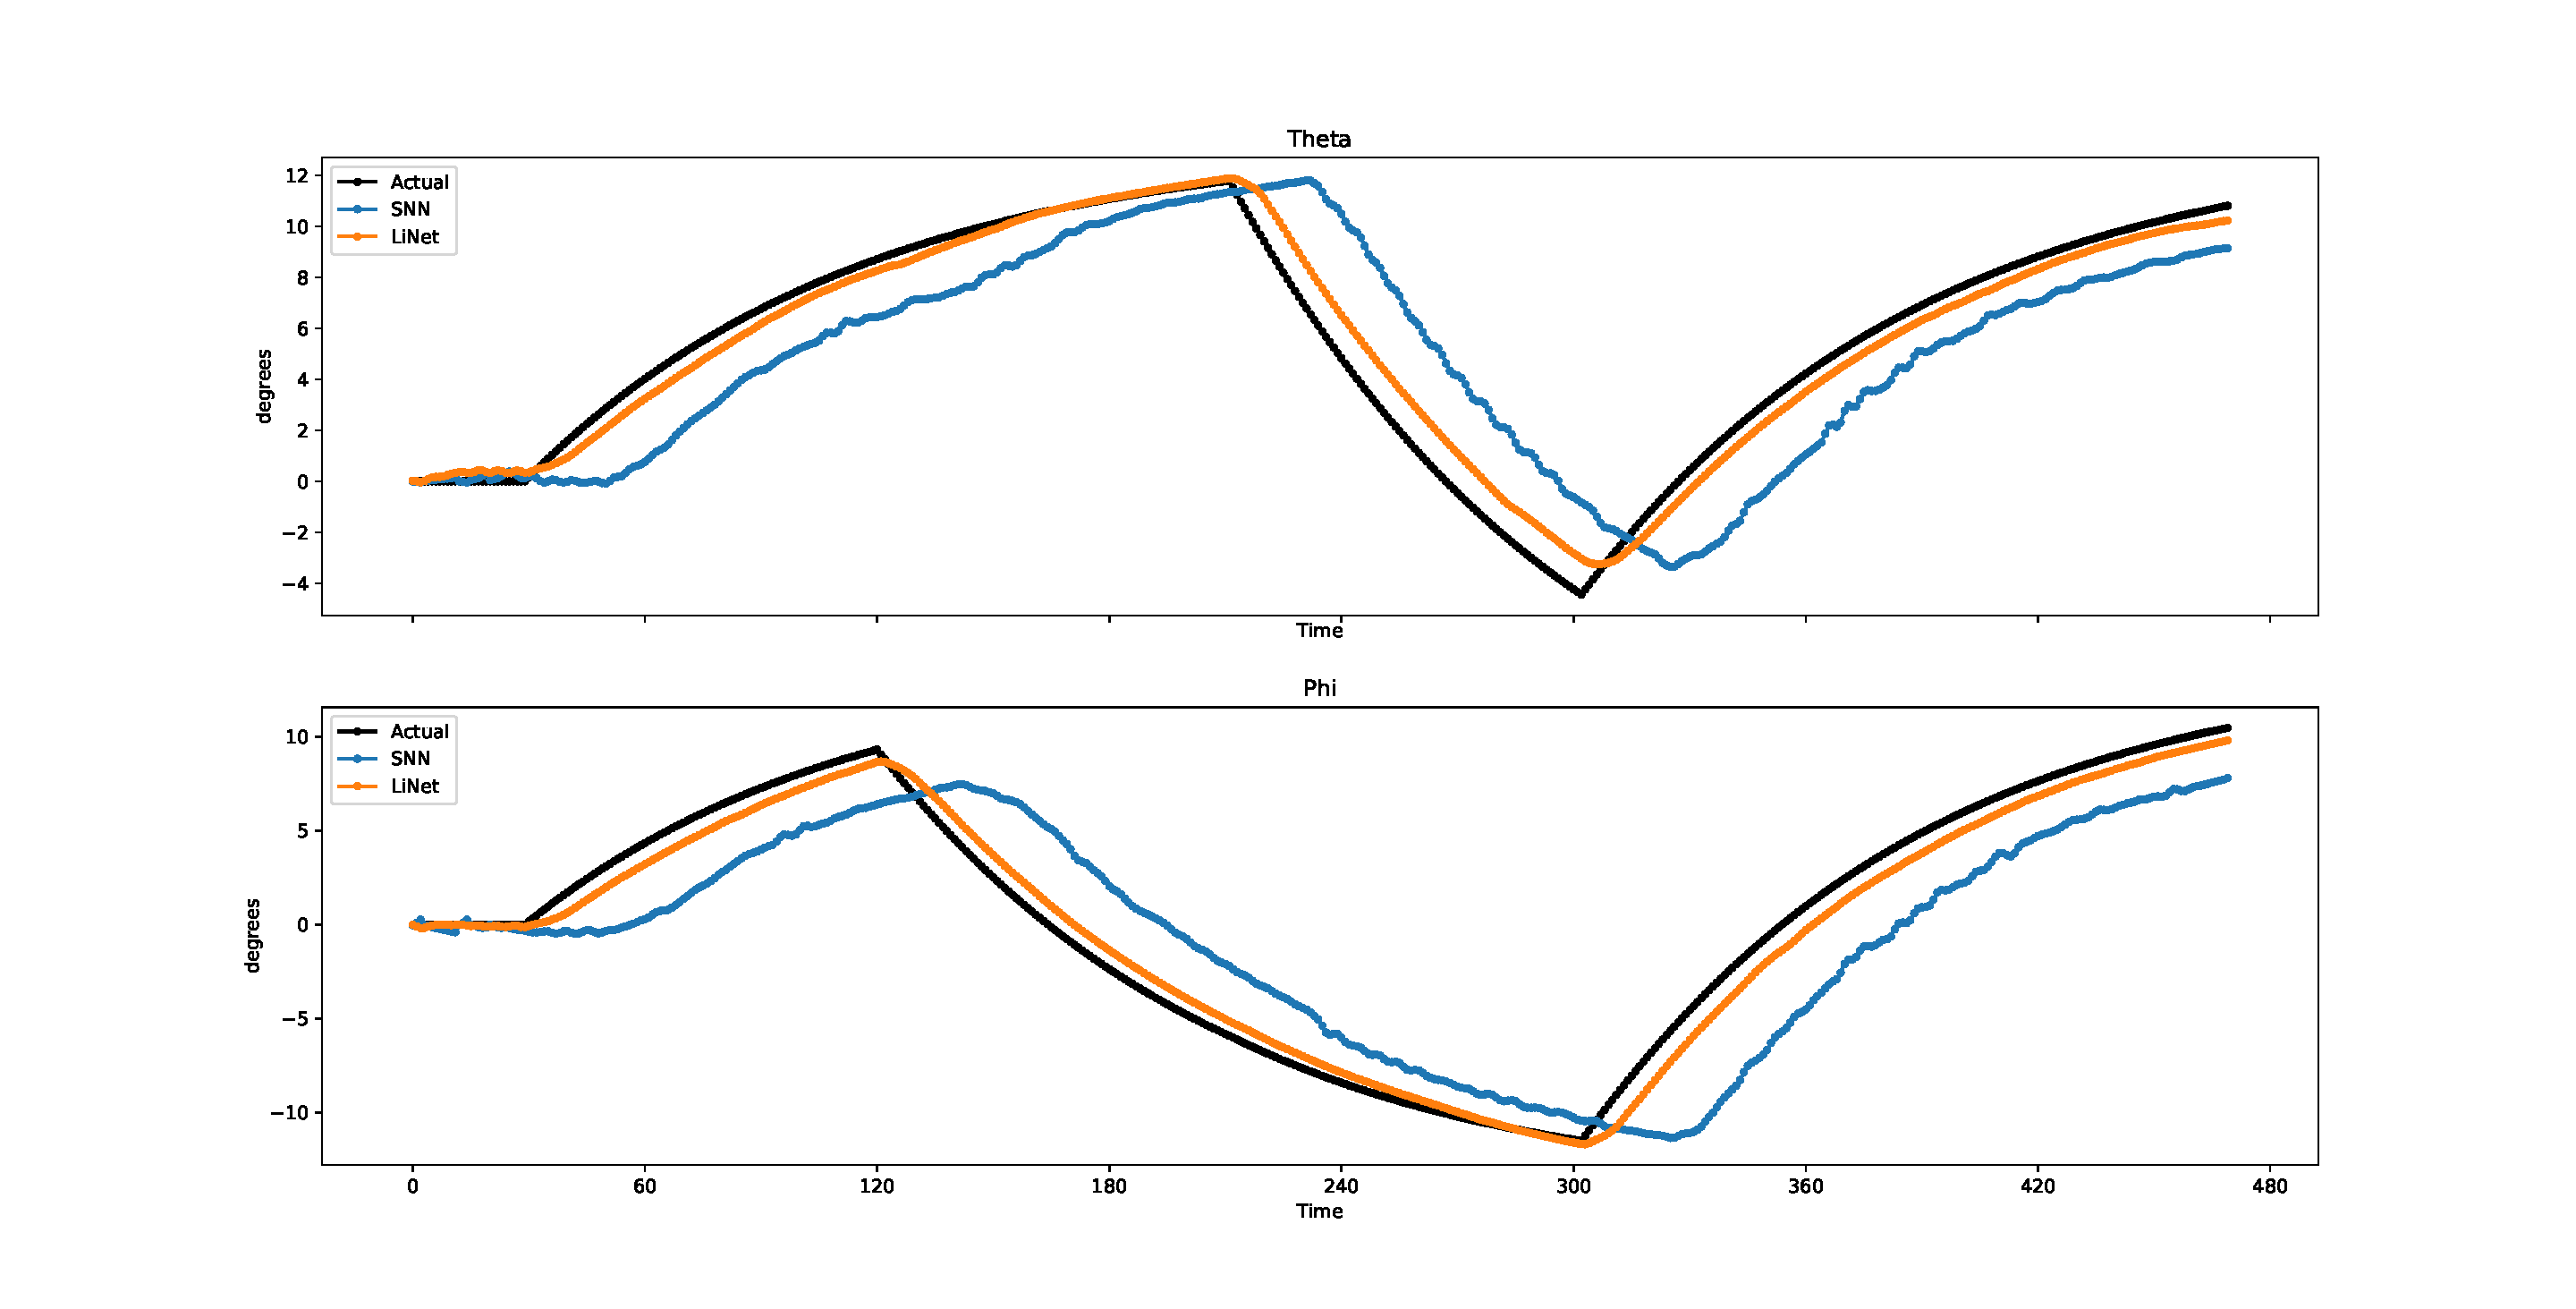
\includegraphics[width=\textwidth]{smooth_normal}
        \caption{}
        \label{fig:smooth_normal}
    \end{subfigure}

    \begin{subfigure}[b]{0.8\textwidth}
        \centering
        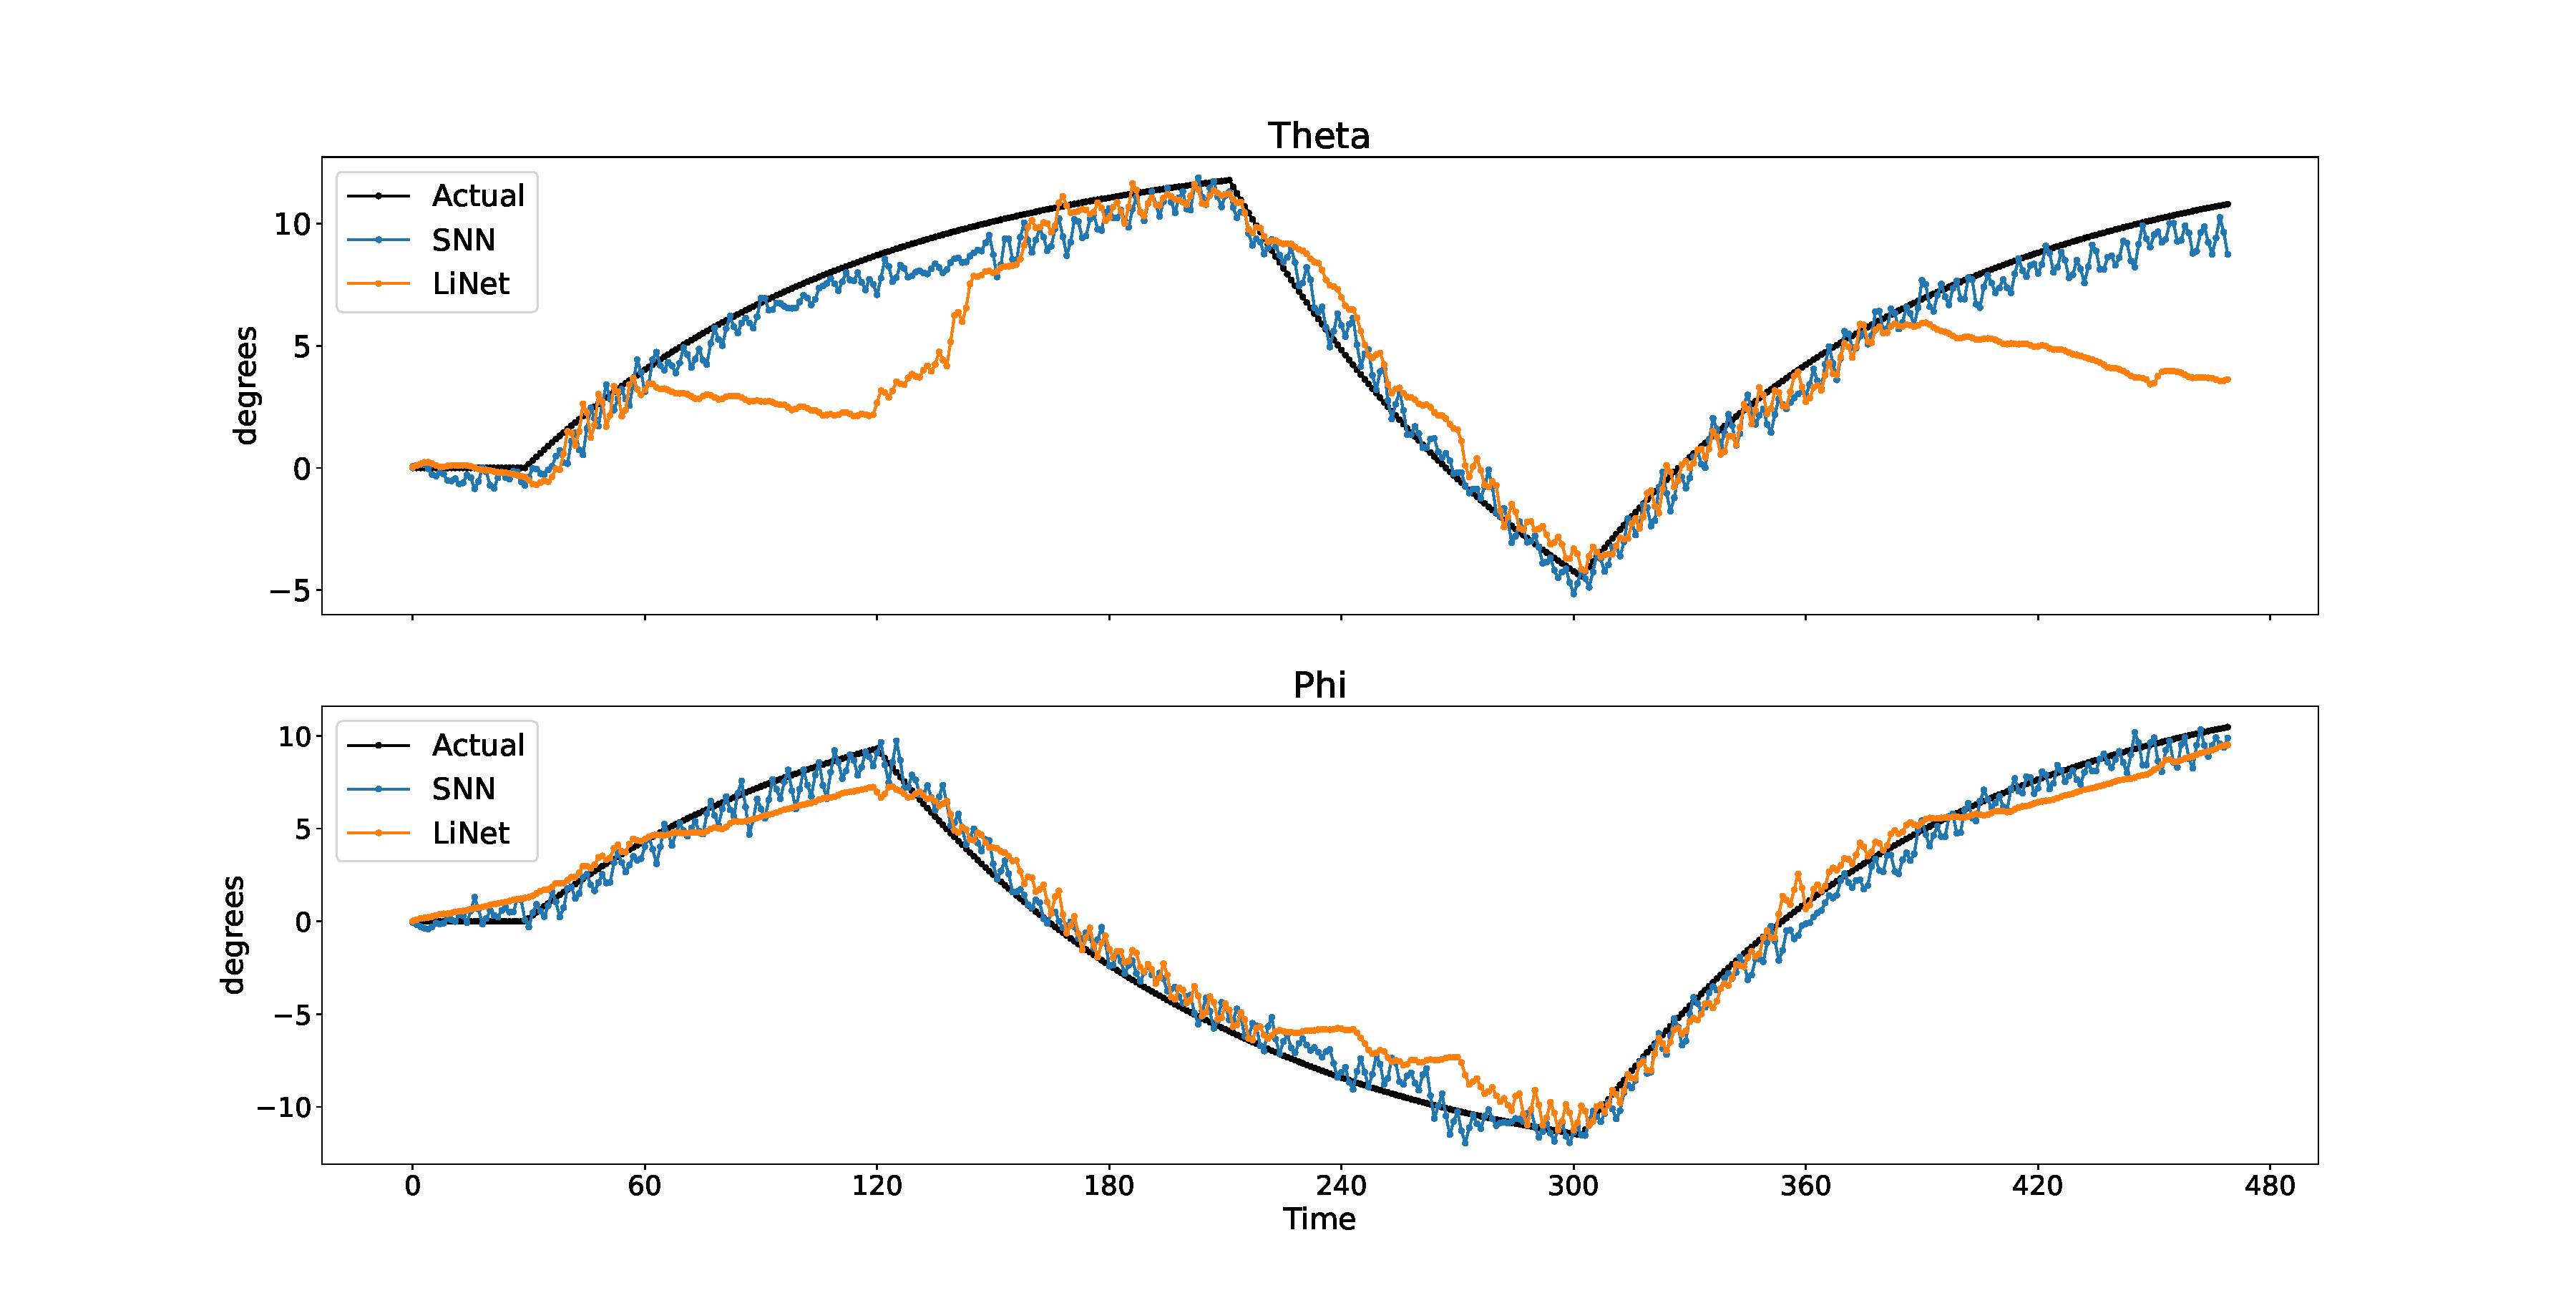
\includegraphics[width=\textwidth]{smooth_delta}
        \caption{}
        \label{fig:smooth_delta}
    \end{subfigure}


    \caption[Smooth pursuit eye orientation with different models]{We compare the output angles of the foveation controller in (a) and the orientation of the center of the eye in (b). The black line represents the expected output based on inverse dynamic simulation.}
    \label{fig:smooth}
\end{figure}

Our SNN, while noisy, tracks the target successfully. It also keeps the target in the center of the fovea when using the delta ONV.

%********************************************************************%

\section{Saccade}

In a real saccade, the eye move rapidly in different directions. To re-create this movement, we allow the eye to fixate on the ball and then rapidly move it to a new point within the eye's field of view. 

In Figure~\ref{fig:saccade} we again compare the performance of a LiNet to that of our 4 layer SNN and Hybrid SNN.
In Figure~\ref{fig:saccade_normal} we compare the performance on the normal ONV. The LiNet performs much better here. In Figure~\ref{fig:saccade_delta} the SNN performs better with a delta ONV but we note that the motions are more noisy. 
% Finally, in Figure~\ref{fig:saccade_hybrid} we again note that our Hybrid SNN creates smooth tracking motions while using the delta ONV.

\begin{figure}
    \centering

    \begin{subfigure}[b]{0.8\textwidth}
        \centering
        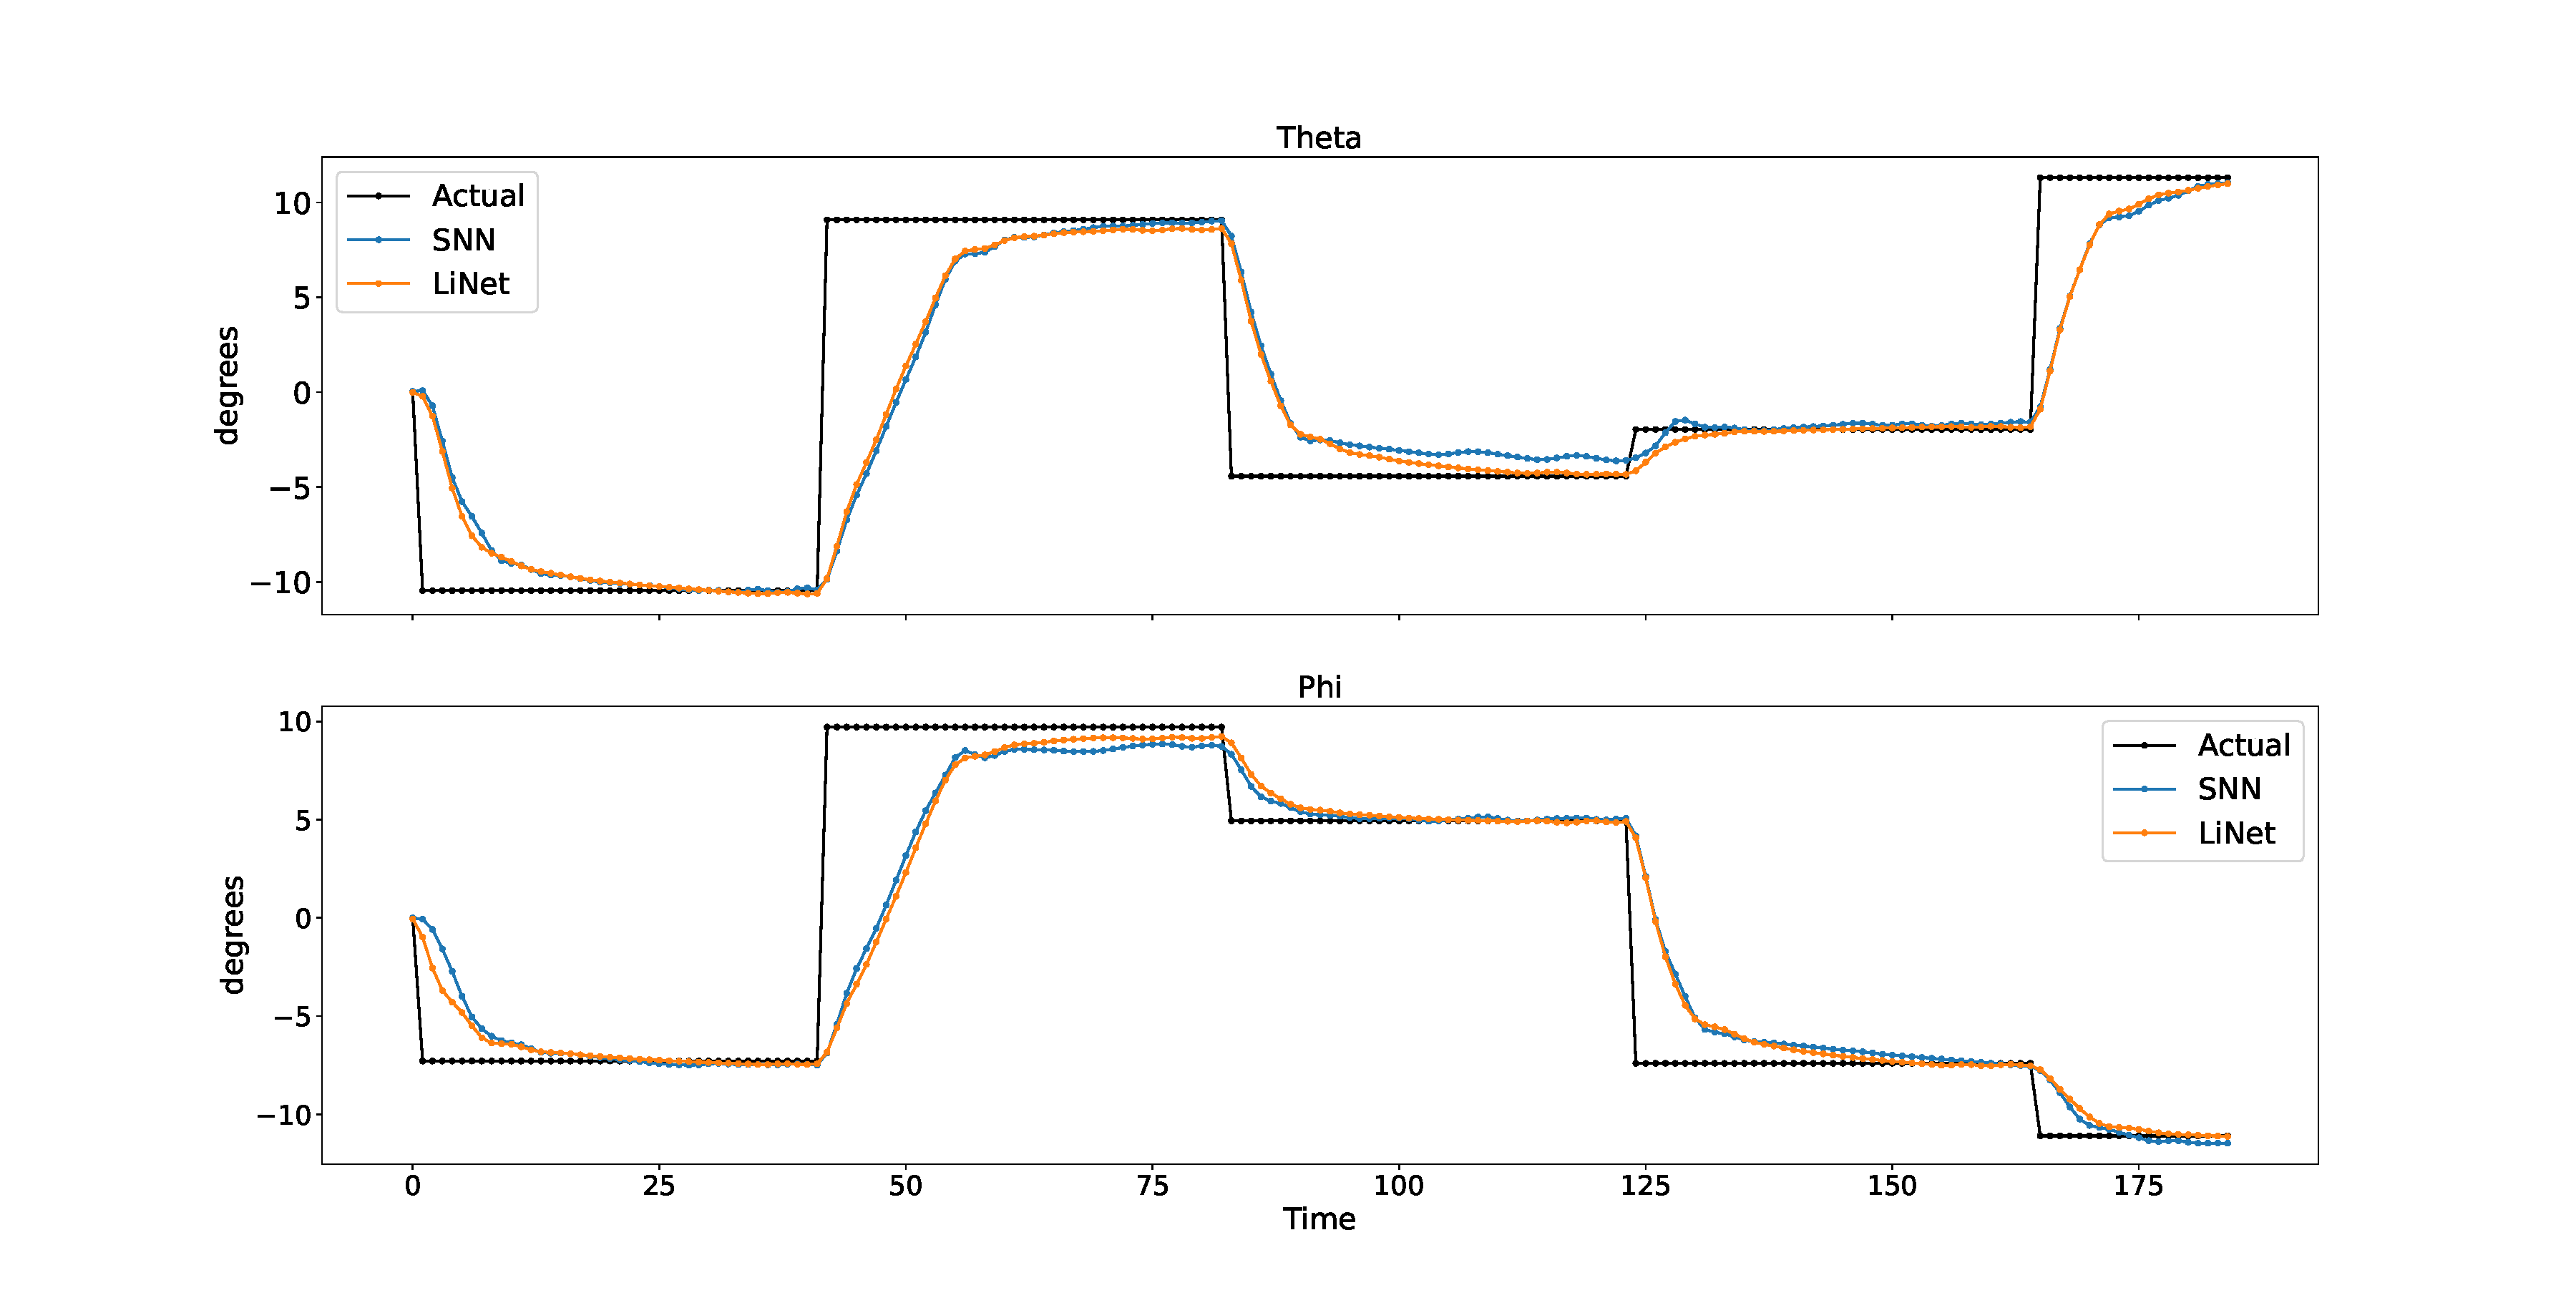
\includegraphics[width=\textwidth]{saccade_ori_normal}
        \caption{}
        \label{fig:saccade_normal}
    \end{subfigure}

    \begin{subfigure}[b]{0.8\textwidth}
        \centering
        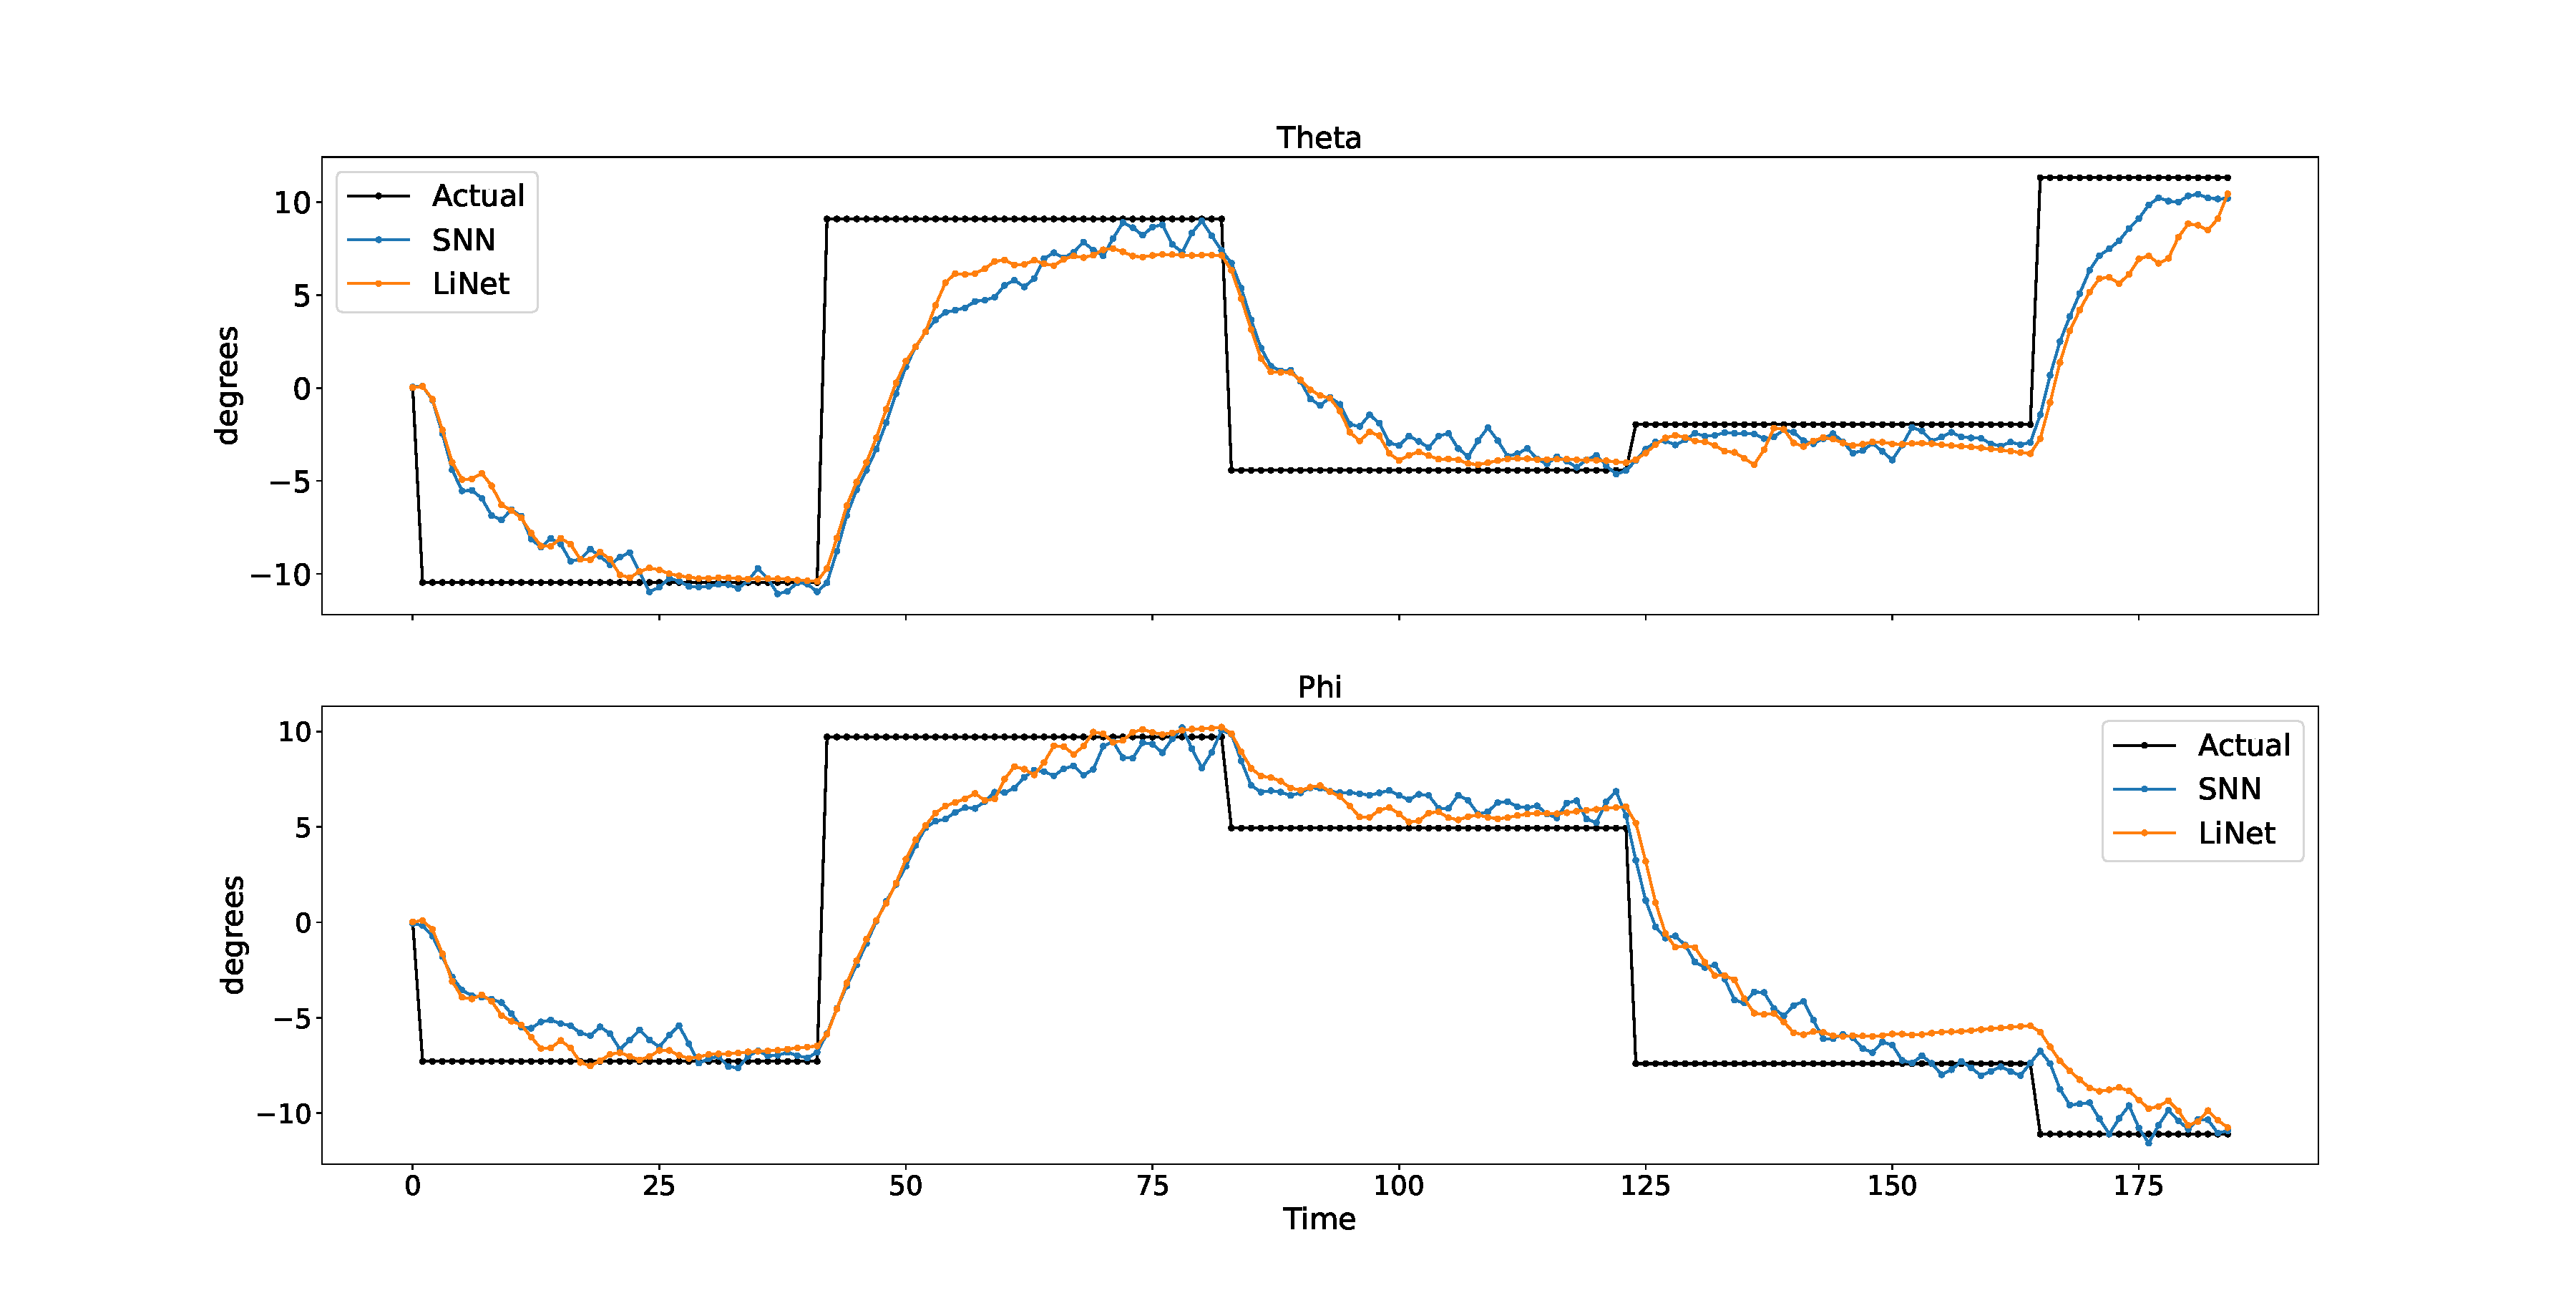
\includegraphics[width=\textwidth]{saccade_ori_delta}
        \caption{}
        \label{fig:saccade_delta}
    \end{subfigure}

    \caption[Saccade eye orientation with different models]{We compare the output angles of the foveation controller in (a) and the orientation of the center of the eye in (b). The black line represents the expected output based on inverse dynamic simulation.}
    \label{fig:saccade}
\end{figure}

Our SNN, while noisy, tracks the target successfully. It also keeps the target in the center of the fovea when using the delta ONV.

% We also use the saccade test to evaluate how realistic our eye movements are.

\begin{figure}
    \centering

    \begin{subfigure}[b]{0.2\textwidth}
        \centering
        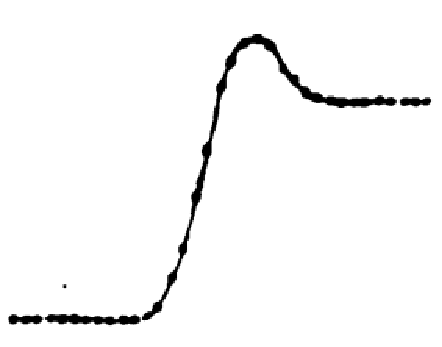
\includegraphics[width=\textwidth]{saccade_human_ori}
        \caption{}
        \label{fig:saccade_human_ori}
    \end{subfigure}
    \hfill
    \begin{subfigure}[b]{0.2\textwidth}
        \centering
        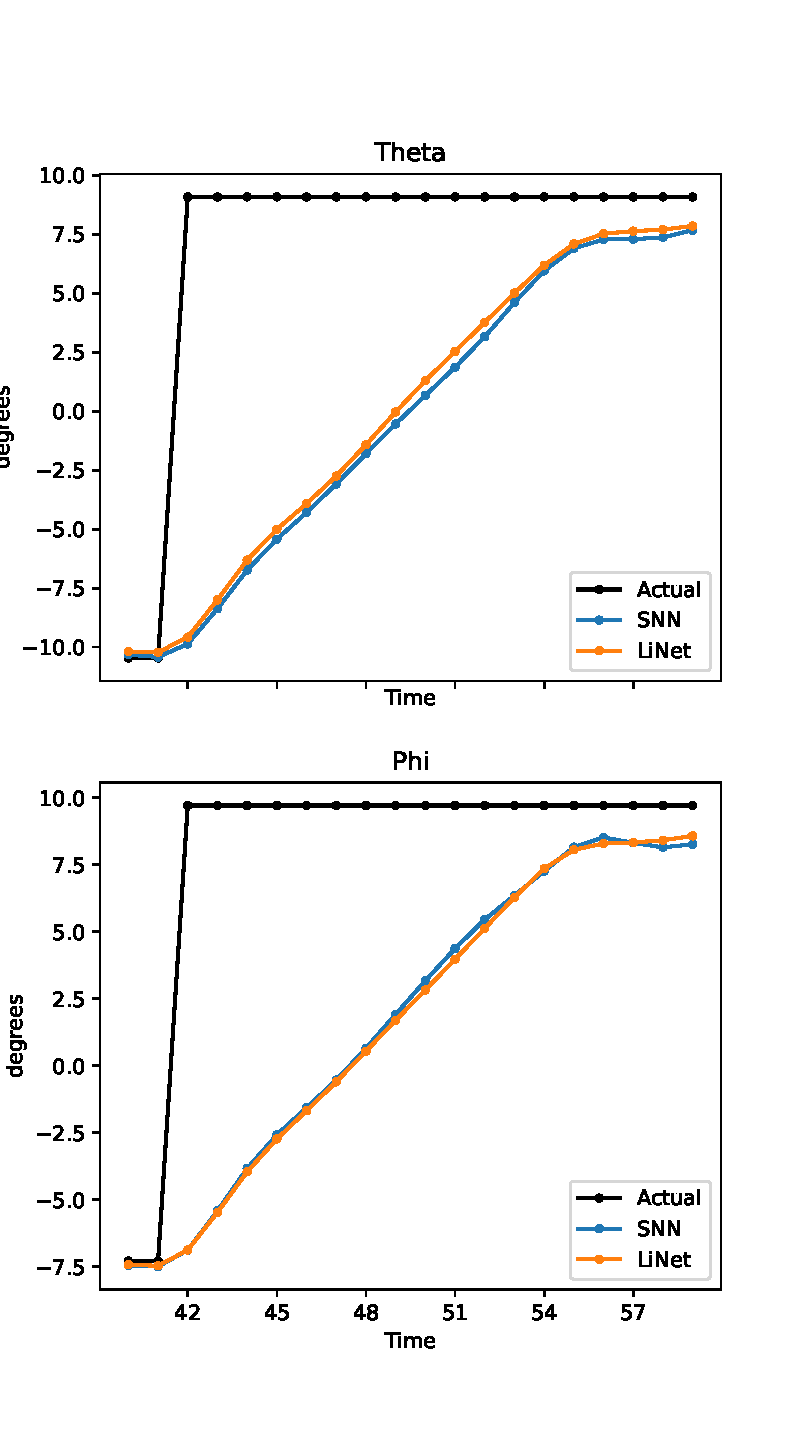
\includegraphics[width=\textwidth]{saccade_human_ori_normal}
        \caption{}
        \label{fig:saccade_human_ori_normal}
    \end{subfigure}
    \hfill
    \begin{subfigure}[b]{0.2\textwidth}
        \centering
        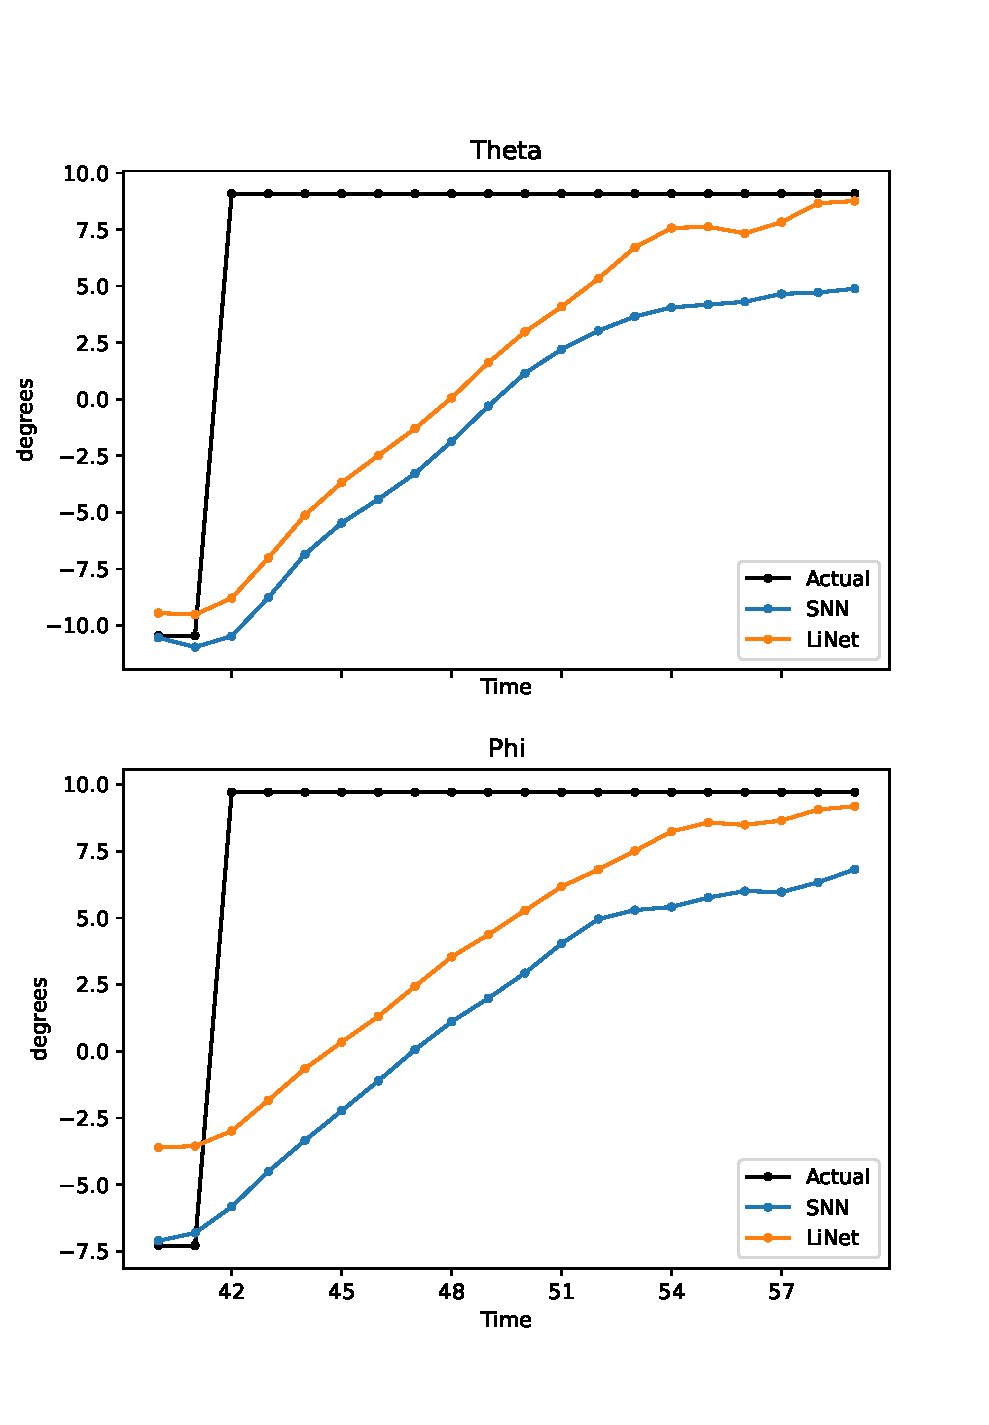
\includegraphics[width=\textwidth]{saccade_human_ori_delta}
        \caption{}
        \label{fig:saccade_human_ori_delta}
    \end{subfigure}

    \caption[]{}
    \label{fig:saccade_ori}
\end{figure}

\begin{figure}
    \centering

    \begin{subfigure}[b]{0.2\textwidth}
        \centering
        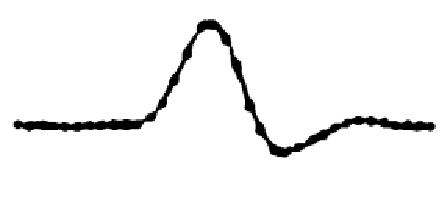
\includegraphics[width=\textwidth]{saccade_human_vel}
        \caption{}
        \label{fig:saccade_human_vel}
    \end{subfigure}
    \hfill
    \begin{subfigure}[b]{0.2\textwidth}
        \centering
        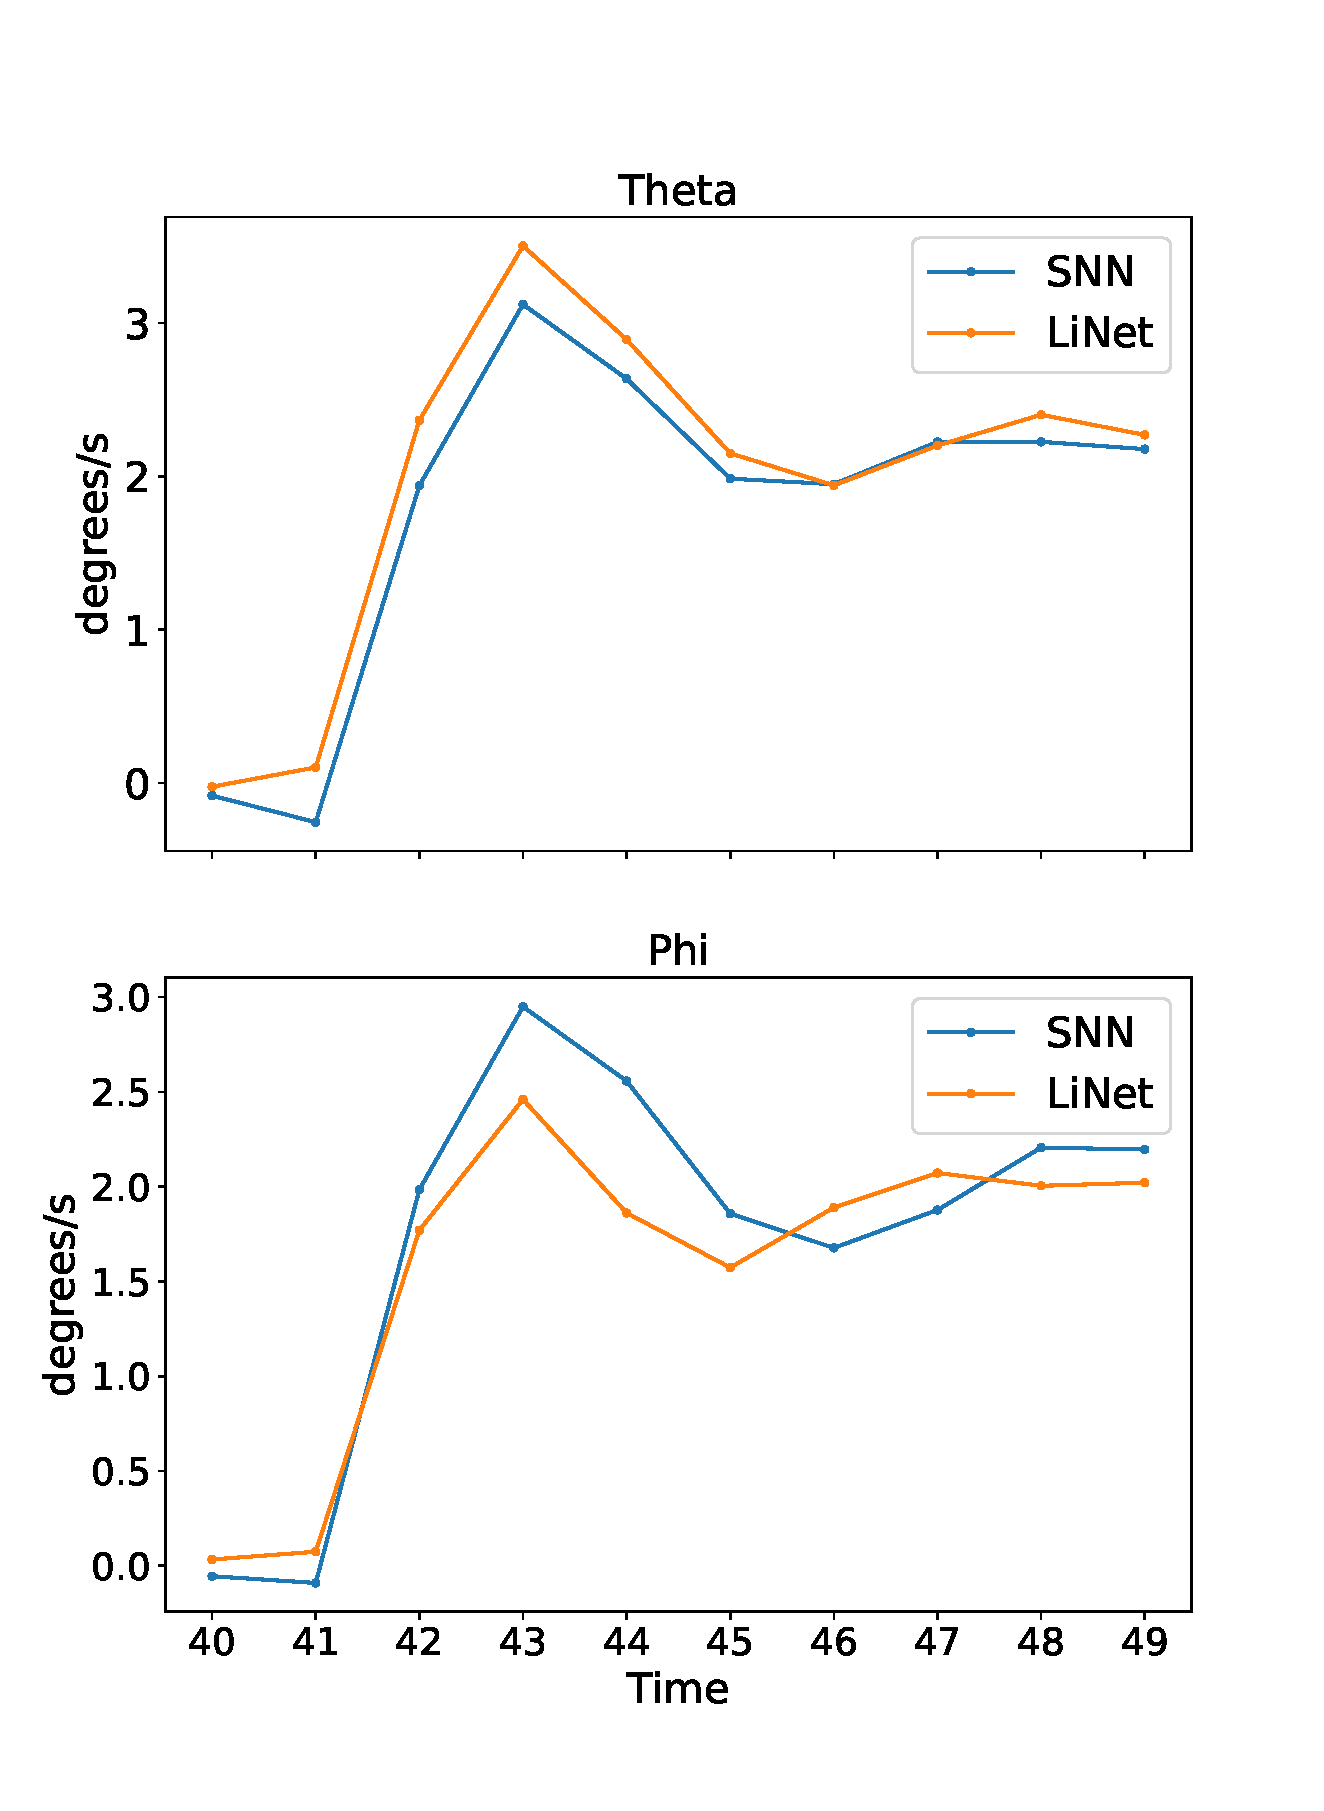
\includegraphics[width=\textwidth]{saccade_human_vel_normal}
        \caption{}
        \label{fig:saccade_human_vel_normal}
    \end{subfigure}
    \hfill
    \begin{subfigure}[b]{0.2\textwidth}
        \centering
        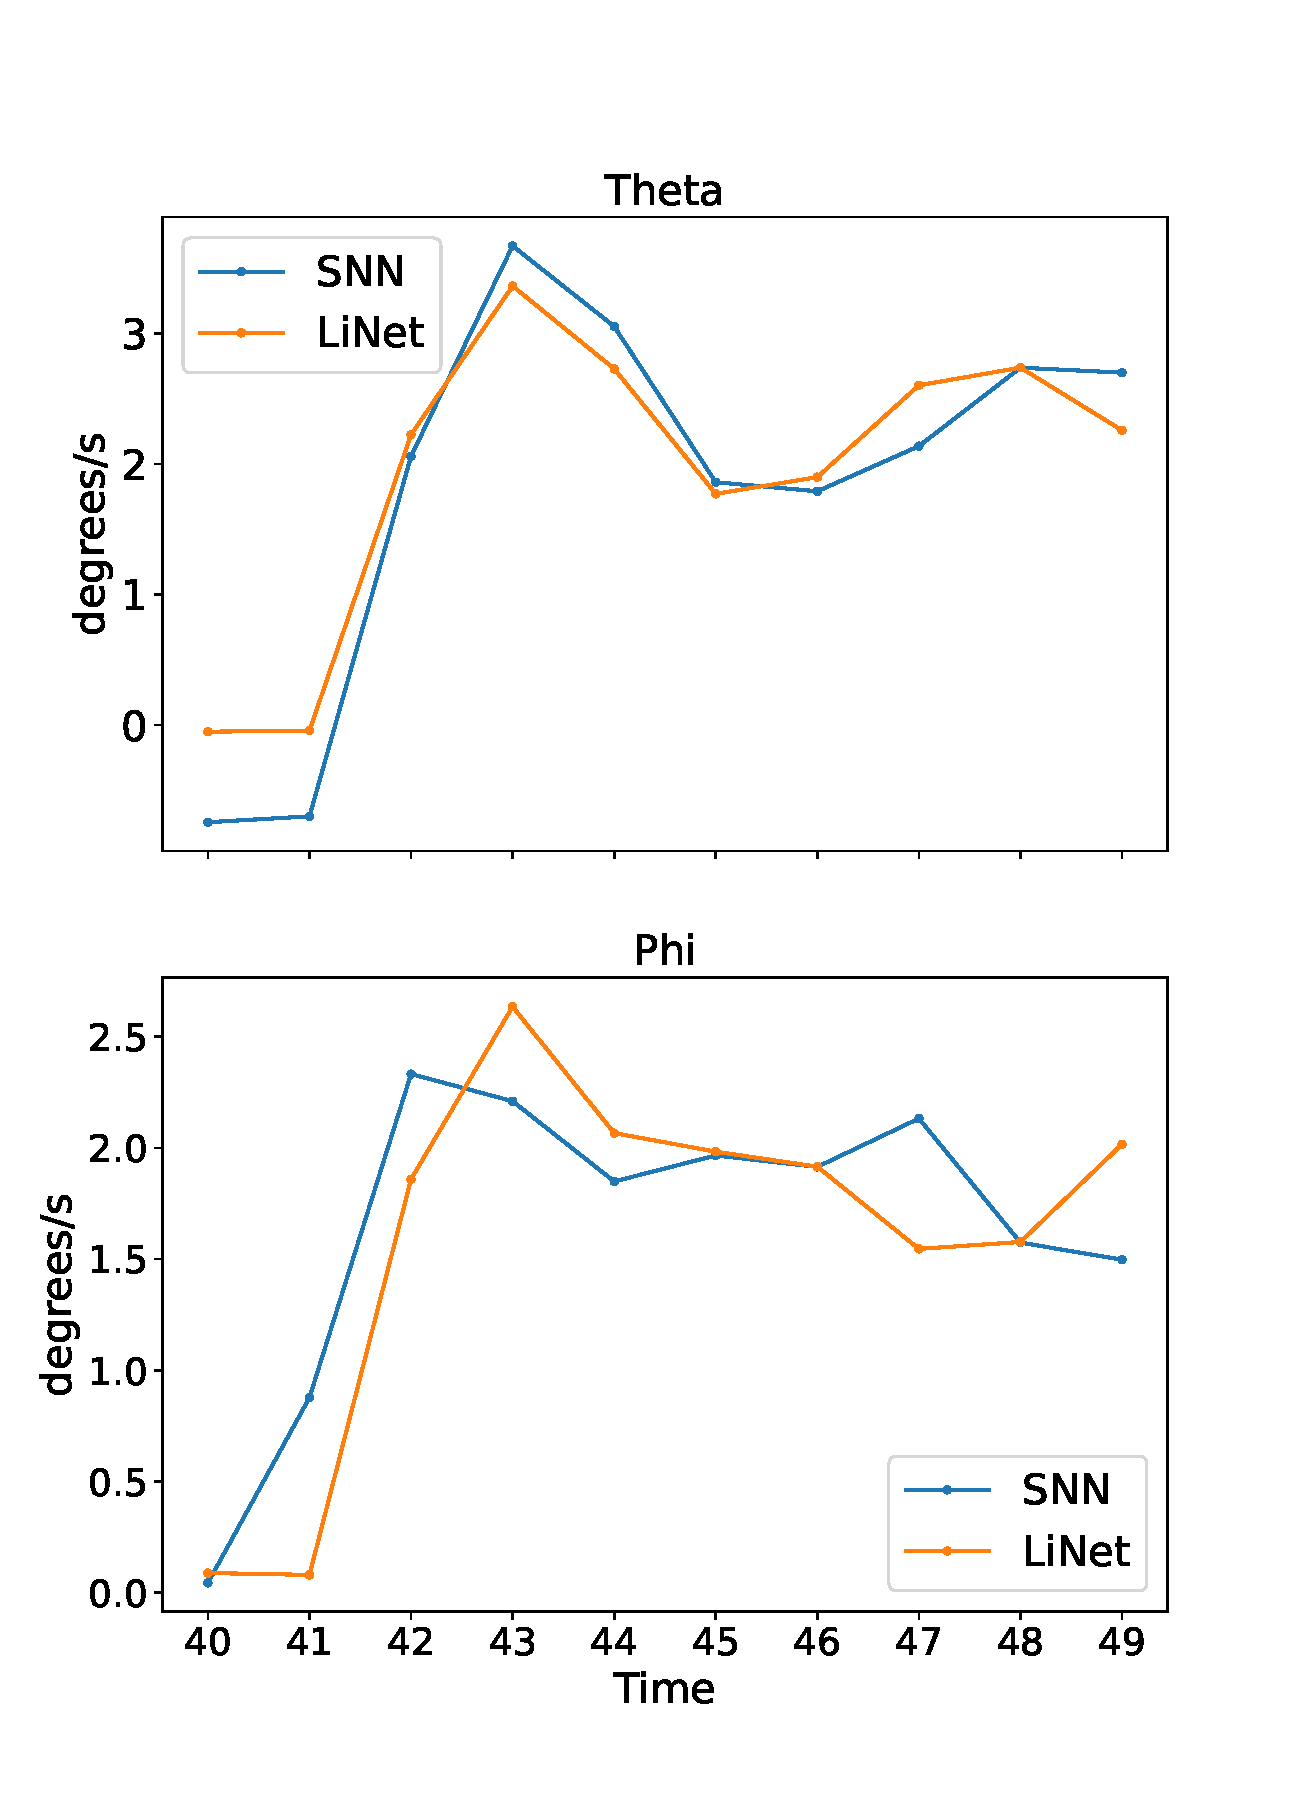
\includegraphics[width=\textwidth]{saccade_human_vel_delta}
        \caption{}
        \label{fig:saccade_human_vel_delta}
    \end{subfigure}

    \caption[]{}
    \label{fig:saccade_vel}
\end{figure}

\begin{figure}
    \centering

    \begin{subfigure}[b]{0.2\textwidth}
        \centering
        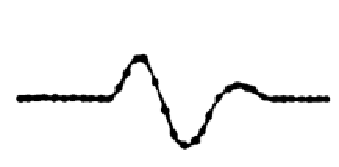
\includegraphics[width=\textwidth]{saccade_human_acc}
        \caption{}
        \label{fig:saccade_human_acc}
    \end{subfigure}
    \hfill
    \begin{subfigure}[b]{0.2\textwidth}
        \centering
        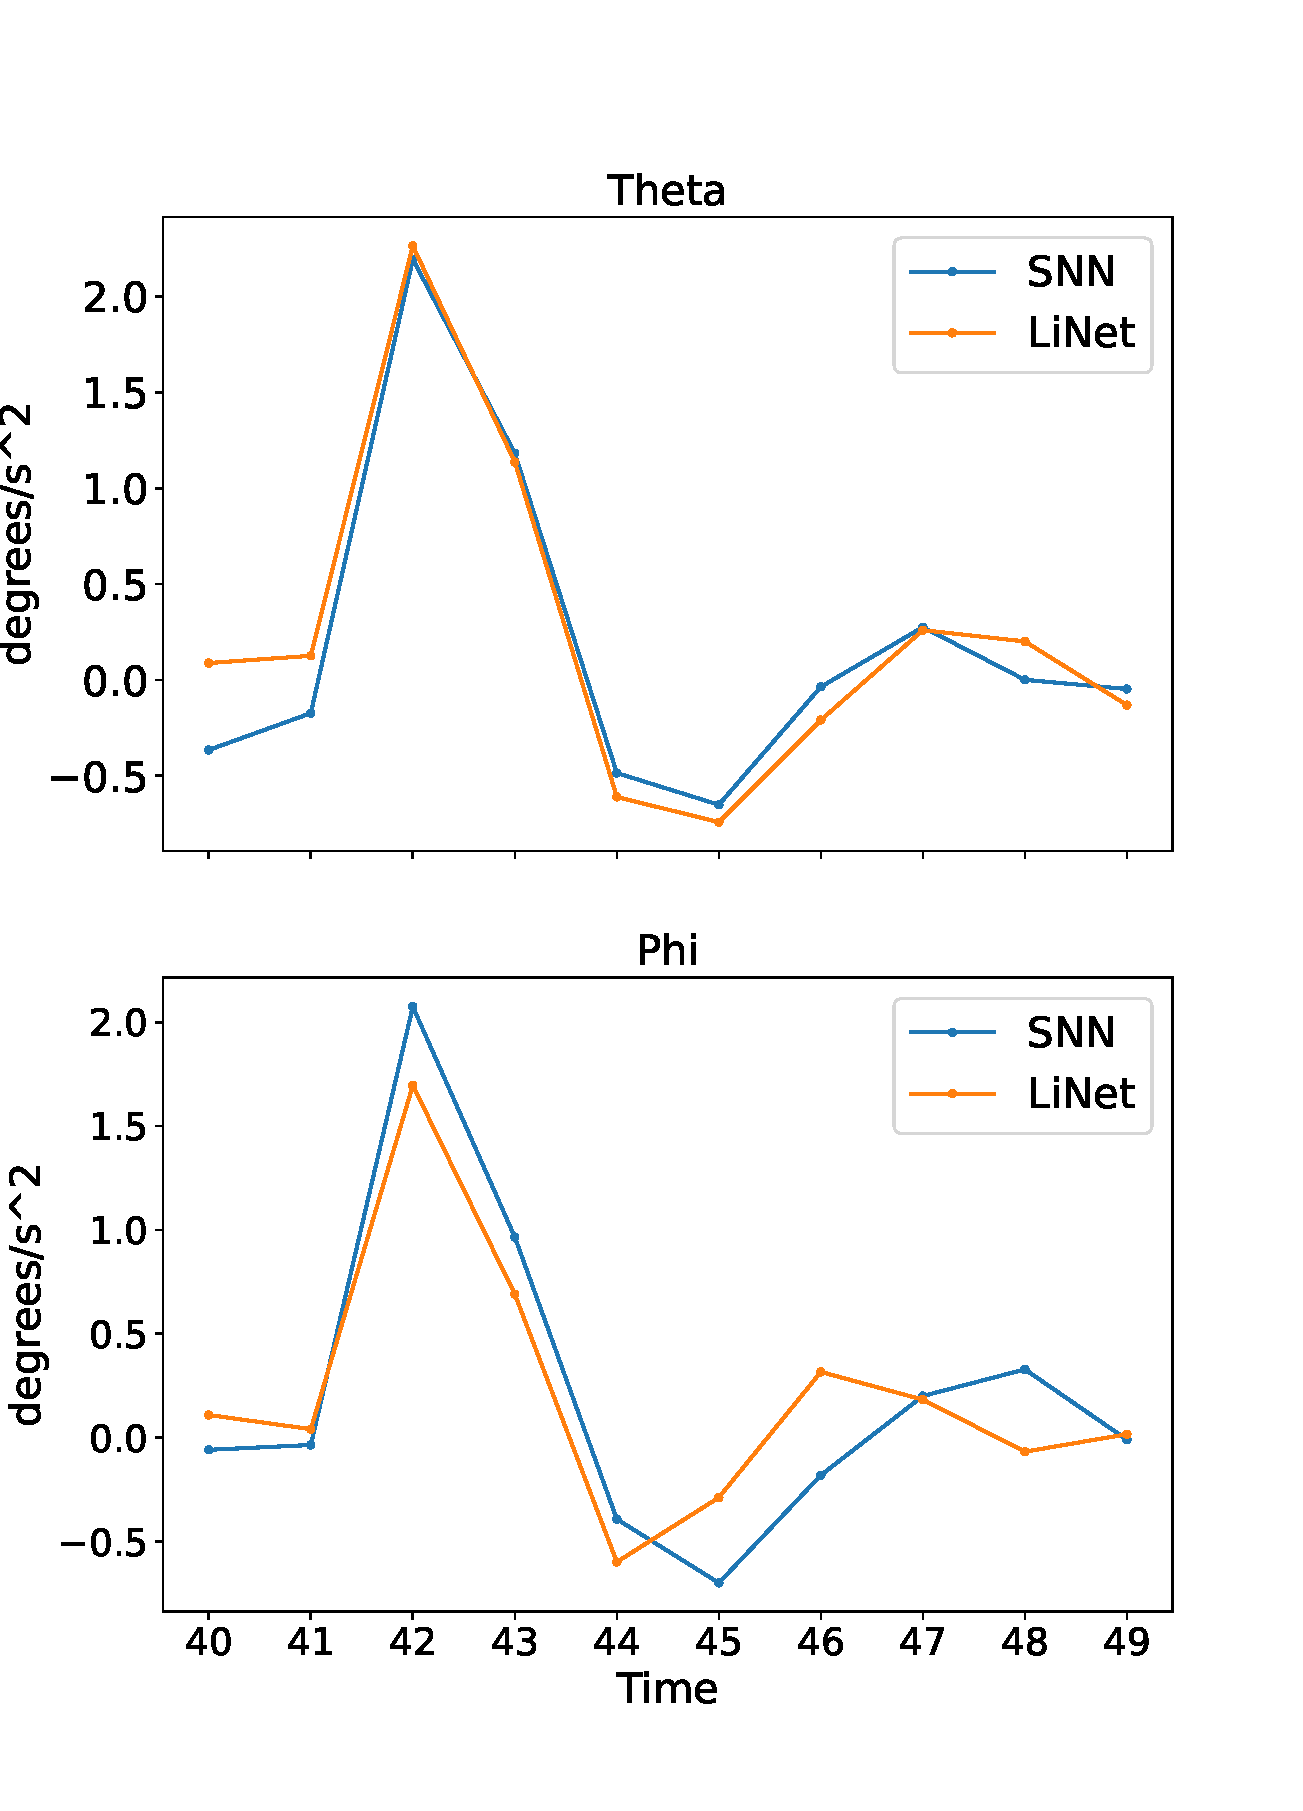
\includegraphics[width=\textwidth]{saccade_human_acc_normal}
        \caption{}
        \label{fig:saccade_human_acc_normal}
    \end{subfigure}
    \hfill
    \begin{subfigure}[b]{0.2\textwidth}
        \centering
        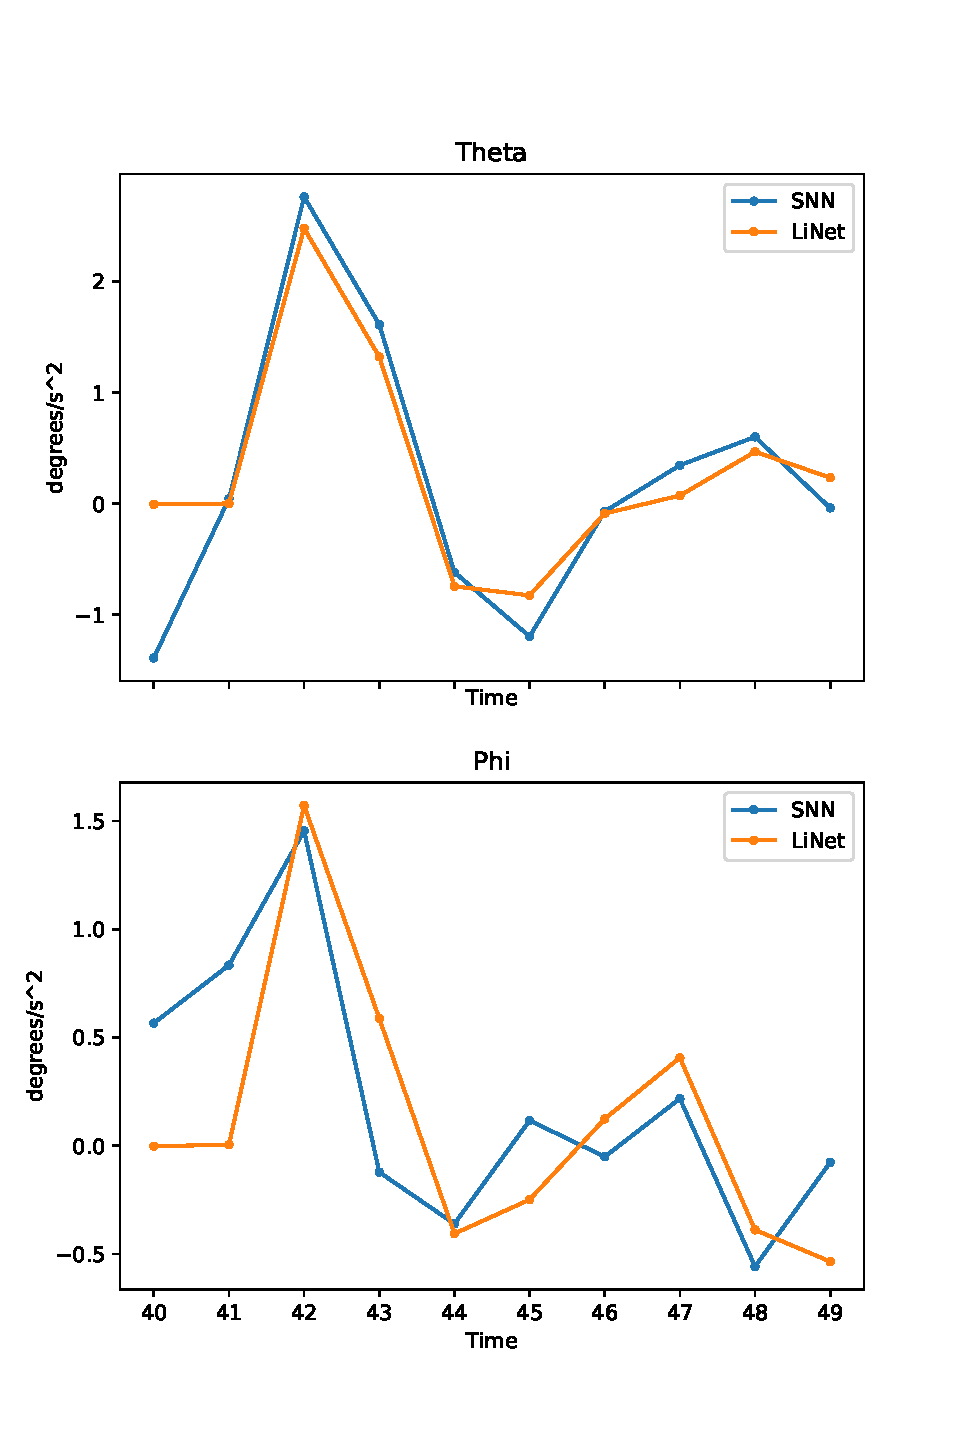
\includegraphics[width=\textwidth]{saccade_human_acc_delta}
        \caption{}
        \label{fig:saccade_human_acc_delta}
    \end{subfigure}

    \caption[]{}
    \label{fig:saccade_acc}
\end{figure}

%********************************************************************%

% \section{Projectile Motion}

%********************************************************************%

% \section{SNN Analysis}

% look at thresholds, membranes, spike rates?

%********************************************************************%

% compare membrane voltage graphs to actual retinal spikes?

% Tables for test set performance

% \begin{center}
% \begin{tabular}{||c c c c c c||} 
%  \hline
%  Model & 0.5 & 0.1 & 0.01 & 0.001 & 0.0001\\ [0.5ex] 
%  \hline\hline
%  LiNet & 99.8 & 95.12 & 5.92 & 0.04 & 0 \\ 
%  \hline
%  Hybrid SNN & 99.8 & 94.28 & 9.08 & 0.12 & 0 \\
%  \hline
%  SNN & 98.76 & 56.08 & 1.36 & 0 & 0 \\[1ex] 
%  \hline
% \end{tabular}
% \end{center}

%%%%%%%%%%%%%%%%%%%%%%%%%%%%%%%%%%%%%%%%%%%%%%%%%%%%%%%%%%%%%%%%%%%%%%

\chapter{Conclusion}

We've brought two important additions to the biomimetic eye model. First, we create a spiking neural network to replace the foveation controller. We use an encoding method that allows for sparse computation and emulates what we believe happens to light at the retina. In addition, training an SNN from scratch with backpropagation to solve a regression task is a novel accomplishment. Our Hybrid SNN architecture allows the user to make a trade off between added noise and more efficient inference. Finally, we've trained our SNN on event-based data, allowing the eye to focus on changes in the scene when performing object tracking.

%********************************************************************%

\section{Discussion}

It makes sense to see more noisy motion from the models trained on delta ONVs
as the eye tries to move to make sure that the ball is in the middle. If the eye stays
still, then there will be no input events and it won't know where the ball is.

It is interesting that the use of just one ReLU layer in the Hybrid SNN allows for very similar performance to that of a LiNet. Our SNN model still performs well but exhibits more side to side motions. The SNN model is great for biological plausibility, but the Hybrid SNN allows for more efficient inference with most of the advnatages of an SNN.

%********************************************************************%

\section{Future Work}

% replace other NNs with SNNs

Many learning techniques are being studied outside of standard backpropagation. This includes spike time dependent plasticity (STDP), which is inspired by a theory of how neurons in the brain reinforce certain pathways. More experimental network layers such as neuron ensembles with inhibition in \citet{nengo} can also inspire more biologically plausible networks and help identify how parts of the visual cortex work.

Given the difficulty of working with the unstructured ONV input, we would like to see if SNNs can be trained on classification tasks with this eye model. This would simulate reading and be an interesting experiment. Some work has been done on PI-MNSIT \citep{}. Furthermore, finding one architecture to do both object tracking and classification would be closer to simulating the visual system.

Finally, the work of this thesis was simulated on a GPU. Given access to neuromorphic hardware, we would like to verify the power and latency improvements proposed by our hybrid SNNs. Perhaps training with neuromorphic chips can open up new possibilities related to training.

%%%%%%%%%%%%%%%%%%%%%%%%%%%%%%%%%%%%%%%%%%%%%%%%%%%%%%%%%%%%%%%%%%%%%%

\appendix

%%%%%%%%%%%%%%%%%%%%%%%%%%%%%%%%%%%%%%%%%%%%%%%%%%%%%%%%%%%%%%%%%%%%%%

\chapter{The Eye Model}
\label{appendix:eye}

In this appendix we offer more detail about the other subsystems of the biomimetic eye model of \citet{Arjun}. All muscles are simulated as Hill-type muscles. There are two methods of controlling each subsytem: inverse dynamic control and neural networks. Because the work of this thesis deals with the foveation controller, the subsystems in this appendix are all controlled with inverse dynamic control.

Inverse dynamic control starts with computing the position that the eye needs to be in to keep up with the target. Given the current position and desired position, we can compute the angular acceleration needed to complete the movement. With the angular acceleration we can compute the torque that the muscles need to apply and finally reach the muscle activations to feed to the model.

The neural network models output the change in muscle activations needed to compute the movements.

% figures

%********************************************************************%

\section{Iris and Pupil}

Light enters the eye through the pupil, and the iris is the muscle that controls how much light actually makes its way to the retina. The iris is controlled in the simulation by two muscles: the pupillary sphincter, which constricts the pupil, the pupillary dilator, which opens up the pupil. To correctly focus light onto the retina, the pupil constricts when there is a large amount of light and it dilates when there is a low amount. 

One muscle activation value is used to simulate the pupil, where a positive value opens it up and a negative one constricts it. This activation can be determined by a shallow fully connected neural network. 

%********************************************************************%

\section{Lens and Cornea}

The lens and cornea serve to refract light to focus it onto the retina. Similar to the iris, the lens lengthens and shortens. The lens lengthens to focus more distant objects and shortens to focus on closer objects. 

Unlike the iris, the lens is modeled with damped springs. It uses the same shallow neural network architecture as the iris and uses one activation value to control its length.

%********************************************************************%

\section{Extraocular (EOC) Muscles}

This subsystem involves three pairs of muscles which work together to move the eyeball with 3 degrees of freedom. One pair controls horizontal movement, one pair controls vertical movement, and the last pair creates a twisting motion. Each muscle in a pair is allows movement in opposite directions.  

The neural network that controls EOC muscles is a deep, fully connected network. Like the other muscle controllers it outputs an activation value for each muscle that dictates how to either contract or relax.

%%%%%%%%%%%%%%%%%%%%%%%%%%%%%%%%%%%%%%%%%%%%%%%%%%%%%%%%%%%%%%%%%%%%%%

\chapter{LiNets}
\label{appendix:linet}

% [LiNet appendix?] Fast convergence, biologically reasonable, good performance

Convolutional layers have allowed for great progress in computer vision. They improve upon fully
connected layers, where a neuron in a given layer is connected to all neurons in the previous layer. In CNNs, each neuron is only connected to neighboring units in the previous layer. Of course, this ``neighboring'' is dependent on the fact that image inputs are organized in structured arrays. Our ONV is an unstructured input and doesn't naturally lend itself to working with CNNs.

This leaves us to experiment with a fully connected architecture. The only problem is that our ONV is a vector of dimension 43,200. A fully connected model created to process this large of a vector would use a great amount of memory and be slow to train. 

The work of \citet{Masaki} solved this by going back to the idea of locally connected networks. Dubbed a ``LiNet,'' each neuron only processes inputs from photoreceptors that are close to each other. The architecture is summarized in Figure~\ref{fig:linet_rgb}. Furthermore, the number of neurons in each subsequent layer is scaled down by a factor f. The architecture converges very quickly and uses much less memory than a comparable fully connected architecture. In addition, it scales much better to larger numbers of photoreceptors.

\begin{figure}
    \centering
    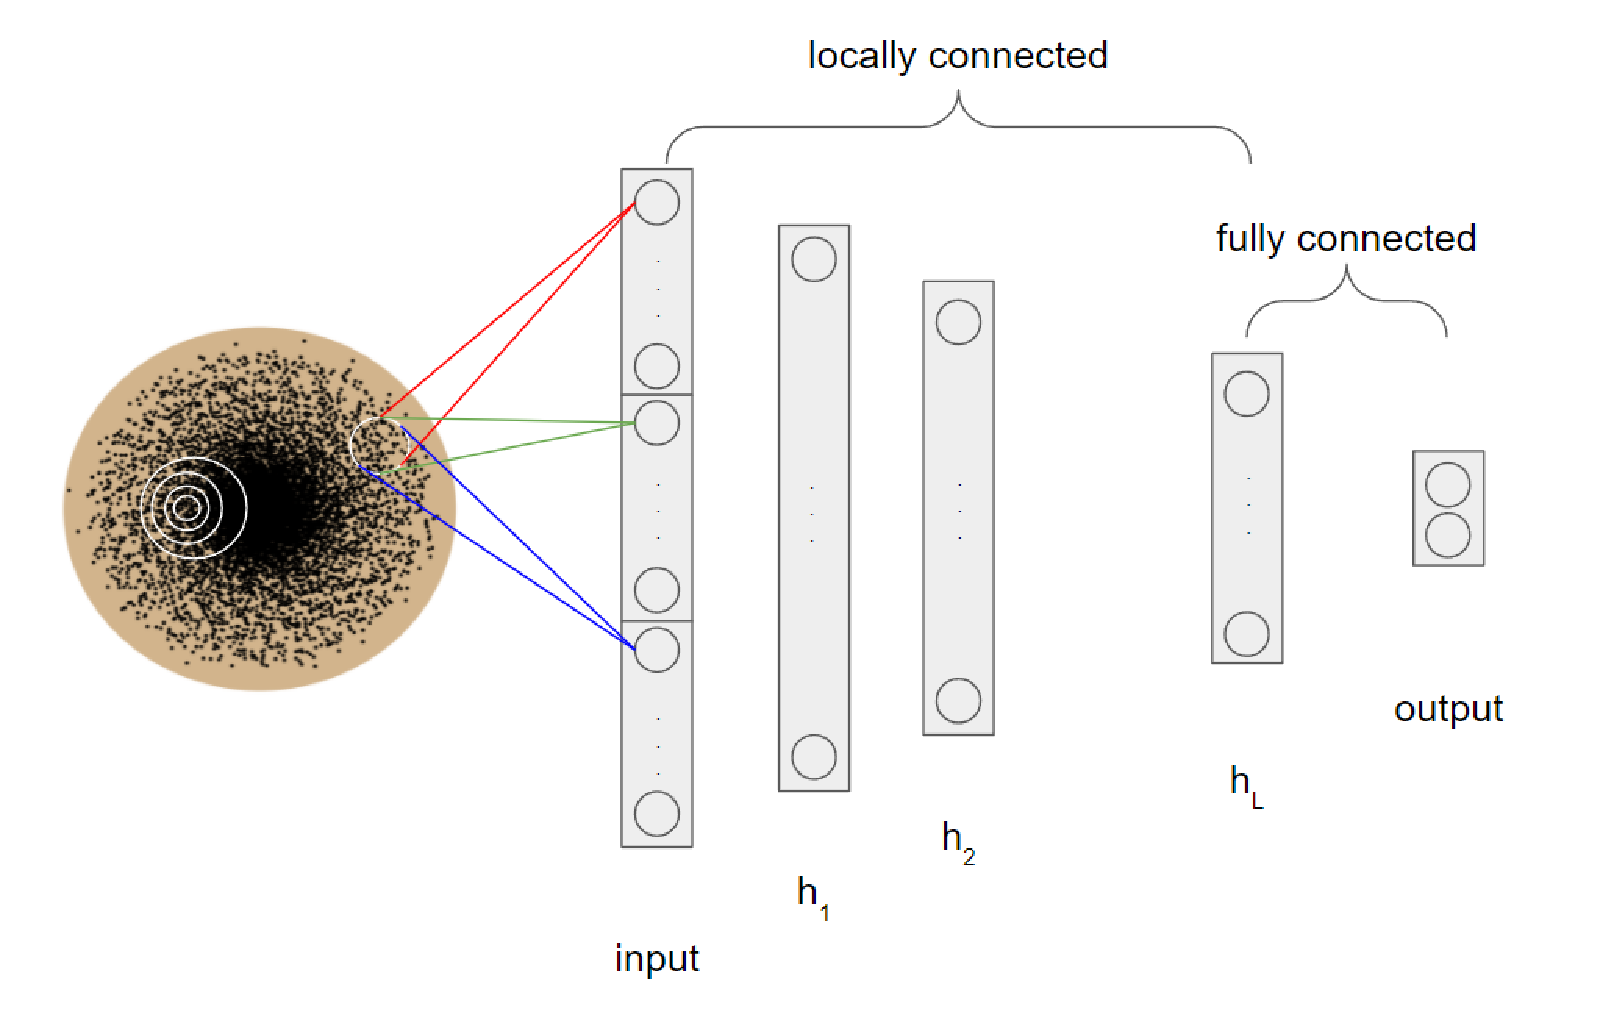
\includegraphics[width=\textwidth]{linet_summary}
    \caption[LiNet architecture summary]{The LiNet architecture. We have a 14,400 photoreceptor retina with red, blue and green channels stacked on top of each other to create the ONV. Each neuron then processes the K nearest red, blue, or green inputs to itNeurons at the first layer combine input from a handful of photoreceptors. Neurons in consecutive layers combine the fields of view from previous layers to slowly get closer to seeing the full scene.}
    \label{fig:linet_rgb}
\end{figure}

Figure~\ref{fig:linet_rgb} also includes white circles to illustrate the advantage of using locally connected networks. The neurons in earlier layers see inputs from a group of neighboring photoreceptors. Neurons in later layers see larger groups of neighboring photoreceptors.

% Image showing neighboring circles getting bigger
% \begin{figure}
%     \centering
%     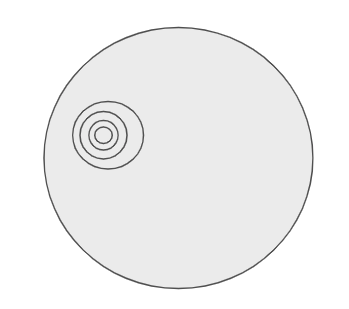
\includegraphics[width=0.5\textwidth]{linet_receptive_fields.png}
%     \caption{}
%     \label{fig:linet_receptive_fields}
% \end{figure}

%********************************************************************%

\section{Training}

We re-train the LiNet architecture as we did not have access to the previously trained model. We collect data points by randomly sampling positions that the target can take in the eye's field of view. Then, through inverse dynamic simulation, we collect the exact angles needed track the target given the current ONV input. Our dataset consisted of 25 thousand datapoints, 2.5 thousand of which were kept for validation and another 2.5 thousand of which were used for testing. 

We kept the 5 layer architecture reported in the original work. We use a factor $f$ of 5, meaning each subsequent layer has half the number of neurons as the previous layer. A number was not reported for $k$, the number of photoreceptors to group together in the input. We conducted a hyperparameter sweep and use a value of 25.

Training was done with a batch size of 16 and a learning rate of 0.001. No regularization is added to the model, and the weights are inialized with He initialization.

%%%%%%%%%%%%%%%%%%%%%%%%%%%%%%%%%%%%%%%%%%%%%%%%%%%%%%%%%%%%%%%%%%%%%%

\chapter{SNN Theory}
\label{appendix:snn}

To implement a SNN, I used a python package built on top of PyTorch called snnTorch \citep{snnTorch}. The main way that SNNs differ from normal artificial neural networks (ANNs) is that the activation function only outputs either a 1 (a ``spike'') or a 0 and that inputs vary over time. Neurons maintain an internal voltage that increases when their inputs spike and decays in the absence of input. This allows SNNs to replace floating point multiplications with simple additions because the synapse weight is only multiplied by a 1 or a 0.

%********************************************************************%

\section{Circuit Model of a Spiking Neuron}

The fundamental unit of an SNN is the leaky integrate and fire (LIF) neuron. It can be represented as an RC circuit as show in Figure~\ref{fig:rc_circuit}.

\begin{figure}
    \centering
    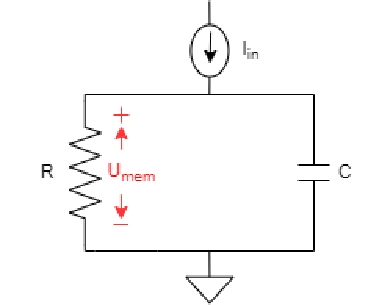
\includegraphics[width=0.5\textwidth]{RC_neuron}
    \caption[RC circuit representation of a LIF neuron]{The RC circuit representing a leaky integrate and fire neuron.}
    \label{fig:rc_circuit}
\end{figure}


From the circuit we can use Kirchoff's current law, and reach the equation below.

$$ I_\text{in}(t) = I_R + I_C $$

Now we want to derive equations for $ I_R $ and $ I_C $. We use Ohm's law, $ I = V/R $, for the resistor and the relationship $ Q = CU_\text{mem}(t) $ for the capacitor. V is the voltage across the resistor and Q is the charge on the capacitor.  

$$ I_R(t) = \frac{U_\text{mem}(t)}{R} $$

$$ I_C(t) = \frac{dQ}{dt} = C \frac{dU_\text{mem}(t)}{dt} $$

Now we place these definitions into our original equation and algebraically solve for $ \frac{dU_\text{mem}(t)}{dt} $.

$$ I_\text{in}(t) = \frac{U_\text{mem}(t)}{R} + C \frac{dU_\text{mem}(t)}{dt} $$
$$ RC \frac{dU_\text{mem}(t)}{dt} = -U_\text{mem}(t) + RI_\text{in}(t)$$

The units of the RHS are in voltage, while the term $\frac{dU_\text{mem}(t)}{dt}$ is voltage/time. Therefore the units of $RC$ must be in time, and we refer to this as the time constant $\tau$. This is a standard ordinary differential equation. We could solve it to get that $ U_\text{mem}(t) = U_0 e ^{\frac{-t}{\tau}} $, but this isn't useful in a discreet time neural network. Therefore, we use the definition of a derivative to get the following form.

$$ \tau \frac{dU(t)}{dt} = -U(t) + RI_\text{in}(t) $$
$$ \tau \frac{U(t + \Delta t) - U(t)}{\Delta t}  = -U(t) + RI_\text{in}(t) $$
$$ U(t + \Delta t) = U(t) + \frac{\Delta t}{\tau} (-U(t) + RI_\text{in}(t)) $$

% Insert graph of decaying membrane w/o input but increasing with input

With this equation we have what we want. A membrane potential that increases with input current and decays in the absence of any input. The equation still has a lot of hyperparameters, which would be very difficult to tune. The snnTorch package simplifies the equation in the following way.

$$ U(t + \Delta t) = (1 - \frac{\Delta t}{\tau}) U(t) + \frac{\Delta t}{\tau} R I_\text{in}(t)$$

Assuming $ I_\text{in}(t) = 0 $.

$$ U(t + \Delta t) = (1 - \frac{\Delta t}{\tau}) U(t) $$

We simplify the term $(1 - \frac{\Delta t}{\tau})$ to $\beta$, the decay rate. Note that $ \Delta t << \tau $ for reasonable accuracy. 

$$ U(t + \Delta t) = \beta U(t) $$

% skipped W derivation, not clear in tutorial
Because we want to work with discreet timesteps, we can assume $\Delta t = 1$. We also assume $R=1$ to reduce the number of hyperparameters. This brings us to the equation

$$ U(t+1) = \beta U(t) + W X(t+1) $$

$W$ is a learnable parameter that weights the input spikes $X$. With $S[t]$ as our spiking function, we add a term to reset the membrane voltage when this neuron outputs a spike. Our final equations are:

$$ U[t+1] = \underbrace{\beta U(t)}_{\text{decay}}
+ \underbrace{W X(t+1)}_{\text{input}}
- \underbrace{S(t)U_\text{thr}}_{\text{reset}} 
$$

$$
S[t] = \begin{cases} 
      1 & \text{if } U(t) > U_\text{thr} \\
      0 & \text{otherwise }
      \end{cases}
$$

%********************************************************************%

\section{Loop Unroll}

From a computational graph perspective, SNNs are very similar to recurrent neural networks (RNNs). This also shows how backpropagation through time (BPTT) can be used to calculate the gradients.

\begin{figure}
    \centering
    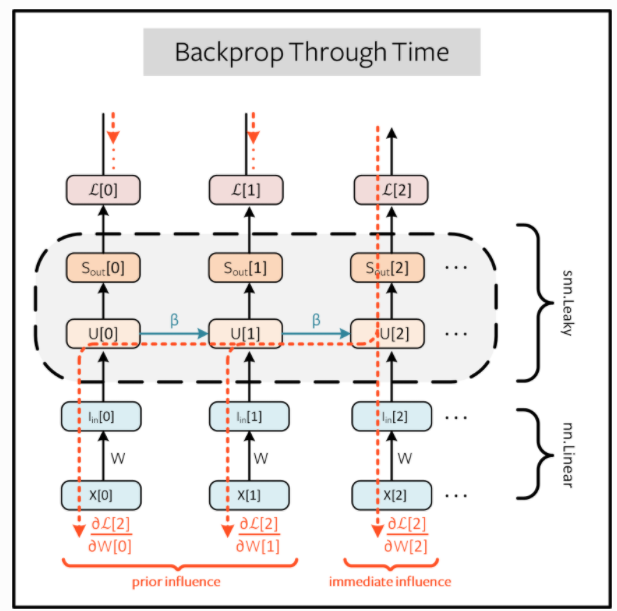
\includegraphics[width=0.8\textwidth]{snnTorch_bptt.png}
    \caption[Unrolled computation graph for a SNN]{Computation graph for a SNN, similar to a RNN. Taken from \citep{snnTorch}.}
    \label{fig:snn_loop_unroll}
\end{figure}

%********************************************************************%

\section{Neuron Parameters}

There are a few choices that we have in the types of neurons that we select to use.

We treat $\beta$ as a hyperparameter, although it can also be trained in different ways. Tuning it on a per-layer or individual neuron basis with backpropagation may be interesting for future work.

The threshold voltage for each neuron is initialized to 1 but is a trainable parameter during backpropagation.

We have two options regarding what to do when the membrane voltage is larger than the threshold voltage. We can either reset the membrane voltage to zero or subtract the threshold voltage from the current membrane voltage. We refer to these techniques as ``reset'' and ``subtract,'' respectively. With the subtract method, the neuron will have a non-zero membrane voltage if it was heavily excited. These methods simulate how a real neuron is inhibited from firing for a short period of time after it spikes. Resetting results in sparser spiking and potential energy savings, but is also more difficult to learn with. We use subtraction in our neurons.

% WTA
Inhibition is another interesting option. In real neurons, sometimes the activation of one neuron can inhibit other neurons from firing. Our more traditional architecture would have very sparse spiking with this type of learning enabled, so it was not used. However, spiking RNNs may benefit from this feature.

Neurons have a distinction between what is known as first and second order. A second order neuron accounts for the fact that when a presynaptic neuron fires, it takes time for the signal to reach the current neuron. This is accounted for by adding a second hyperparameter $\alpha$. These models are more complex to train and resulted in higher loss values, so our work uses first order spiking neurons.

%%%%%%%%%%%%%%%%%%%%%%%%%%%%%%%%%%%%%%%%%%%%%%%%%%%%%%%%%%%%%%%%%%%%%%

\bibliographystyle {UCLAthesis}
\bibliography{thesis}

\end {document}